\PassOptionsToPackage{unicode=true}{hyperref} % options for packages loaded elsewhere
\PassOptionsToPackage{hyphens}{url}
%
\documentclass[
  11pt,
  a4paper,
  DIV=12,captions=tableheading,oneside]{scrbook}
\usepackage{lmodern}
\usepackage{amssymb,amsmath}
\usepackage{ifxetex,ifluatex}
\ifnum 0\ifxetex 1\fi\ifluatex 1\fi=0 % if pdftex
  \usepackage[T1]{fontenc}
  \usepackage[utf8]{inputenc}
  \usepackage{textcomp} % provides euro and other symbols
\else % if luatex or xelatex
  \usepackage{unicode-math}
  \defaultfontfeatures{Scale=MatchLowercase}
  \defaultfontfeatures[\rmfamily]{Ligatures=TeX,Scale=1}
  \setmainfont[]{Times New Roman}
  \setsansfont[]{Lato}
  \setmonofont[]{Source Code Pro}
\fi
% use upquote if available, for straight quotes in verbatim environments
\IfFileExists{upquote.sty}{\usepackage{upquote}}{}
\IfFileExists{microtype.sty}{% use microtype if available
  \usepackage[]{microtype}
  \UseMicrotypeSet[protrusion]{basicmath} % disable protrusion for tt fonts
}{}
\makeatletter
\@ifundefined{KOMAClassName}{% if non-KOMA class
  \IfFileExists{parskip.sty}{%
    \usepackage{parskip}
  }{% else
    \setlength{\parindent}{0pt}
    \setlength{\parskip}{6pt plus 2pt minus 1pt}}
}{% if KOMA class
  \KOMAoptions{parskip=half}}
\makeatother
\usepackage{xcolor}
\IfFileExists{xurl.sty}{\usepackage{xurl}}{} % add URL line breaks if available
\IfFileExists{bookmark.sty}{\usepackage{bookmark}}{\usepackage{hyperref}}
\hypersetup{
  pdfauthor={Florian Hochstrasser},
  pdfborder={0 0 0},
  breaklinks=true}
\urlstyle{same}  % don't use monospace font for urls
\usepackage{longtable,booktabs}
% Allow footnotes in longtable head/foot
\IfFileExists{footnotehyper.sty}{\usepackage{footnotehyper}}{\usepackage{footnote}}
\makesavenoteenv{longtable}
\setlength{\emergencystretch}{3em}  % prevent overfull lines
\providecommand{\tightlist}{%
  \setlength{\itemsep}{0pt}\setlength{\parskip}{0pt}}
\setcounter{secnumdepth}{5}
% Redefines (sub)paragraphs to behave more like sections
\ifx\paragraph\undefined\else
  \let\oldparagraph\paragraph
  \renewcommand{\paragraph}[1]{\oldparagraph{#1}\mbox{}}
\fi
\ifx\subparagraph\undefined\else
  \let\oldsubparagraph\subparagraph
  \renewcommand{\subparagraph}[1]{\oldsubparagraph{#1}\mbox{}}
\fi

% set default figure placement to htbp
\makeatletter
\def\fps@figure{htbp}
\makeatother

%\let\oldmaketitle\maketitle
%\AtBeginDocument{\let\maketitle\relax}

\usepackage{scrhack}
\usepackage{booktabs}
\usepackage{longtable}
\usepackage{array}
\usepackage{multirow}
\usepackage{wrapfig}
\usepackage{float}
\usepackage{colortbl}
\usepackage{pdflscape}
\usepackage{tabu}
\usepackage{threeparttable}
\usepackage{threeparttablex}
\usepackage[normalem]{ulem}
\usepackage{makecell}

\usepackage[font=small]{caption}
\usepackage{subfig}
\usepackage[scaled=0.8]{sourcecodepro}

\usepackage{listings}
\usepackage{subfig}

%% Typography defaults
\usepackage{dsfont}
\usepackage[english]{babel}
\usepackage{microtype} % better management of overfulls

\usepackage[bottom]{footmisc}

% Compact tables
\renewcommand{\arraystretch}{0.9}

% Place figures in current section
\usepackage[section]{placeins}

\providecommand{\tightlist}{%
  \setlength{\itemsep}{0pt}\setlength{\parskip}{0pt}}

\usepackage{graphicx}
\graphicspath{ {./figures/} }

\usepackage{float}

\author{Florian Hochstrasser}
\date{2019-04-24}

\begin{document}

\begin{titlepage}

\titlehead{Master Thesis}
\subject{Profit maximisation for direct marketing campaigns}
\title{An application of knowledge discovery for decision making}
\subtitle{Submitted for the programme Master in Statistics}
\author{Florian Hochstrasser}
\date{14.06.2019}
\publishers{Supervisor: Jacques Zuber}
\extratitle{ }
\uppertitleback{Obiger Titelrückentitel}
\lowertitleback{Für dieses Beispiel wird keine Haftung übernommen.}
\dedication{Dieses Beispiel widme ich\\allen LaTeX Usern}

\end{titlepage}

{
\setcounter{tocdepth}{2}
\tableofcontents
}
\hypertarget{abstract}{%
\chapter*{Abstract}\label{abstract}}
\addcontentsline{toc}{chapter}{Abstract}

It is known that\ldots{}.

This work addressed the problem from the perspective of\ldots{}

It could be shown that\ldots{}

Henceforth, it should be considered that\ldots{}

\hypertarget{intro}{%
\chapter{Introduction}\label{intro}}

A U.S. American veterans organization regularly conducts direct marketing campaigns, asking their members for donations (gifts) for the treatment of veterans with spinal injuries. The goal for the organisation is to maximize the net profit from their campaigns.

Only a small proportion of the members give a gift in reply to a campaign, while each letter sent out has a unit cost of 0.68 \$US. In order to maximize profit, it is therefore desirable to only mail members who are likely to donate.

The members are grouped, among other criteria, by the recency of their last gift. Of these groups, the so-called \emph{lapsed} donors are of particular interest. These are members who made their last gift to the organisation 13 to 24 months prior to a given campaign.
This group is important for two reasons: Firstly, the likelihood of a member donating decreases with the time the member has not donated. Enticing these lapsed donors to give again therefore maintains an active member base. Secondly, the organisation has found that there is a negative correlation between the dollar amount donated and the likelihood to respond to a campaign. This means it is important to include the most unlikely donors in future mailings because if they donate, the net revenue is particularly large. If these unlikely donors would be suppressed from future campaigns, the gains from additional \emph{small dollar} lapsed donors would not offset the losses from the potential \emph{high dollar} donors.

The data at hand was distributed for the purpose of the KDD-CUP of the year 1998\footnote{For an archive of past cups, see \href{http://www.kdd.org/kdd-cup}{SIGKDD - KDD Cup}}. The cup was until recently held yearly under the aegis of the special interest group on Knowledge Discovery and Data Mining (SIGKDD), which itself is part of the Association for Computing Machinery\footnote{\url{https://acm.org}} (ACM).

At the time of the competition, 20 years ago, machine learning was in it's second boom phase. Since then, there was one more period of slump before the current boom that started in the mid-2000's (see Goodfellow, Bengio, and Courville (\protect\hyperlink{ref-Goodfellow-et-al-2016}{2016})). Both computing power and tools available have undergone a substantial transformation since 1998, when the frontrunners in the KDD-CUP competition were all big players in the field, showcasing their proprietary software. This thesis thus also demonstrates the possibilities that are currently at hand, from powerful open-source toolkits like scikit-learn to cloud computing.

\hypertarget{task}{%
\section{Task}\label{task}}

The task for this thesis was to perform a complete data analysis (data preprocessing, model evaluation, model selction, prediction).

A requirement set by the supervisor of this thesis was that the solution be demonstrated using Python (see Rossum (\protect\hyperlink{ref-CS-R9526}{1995})) as a programming environment.

\hypertarget{goal}{%
\section{Goal}\label{goal}}

The ultimate goal was to beat the winner of the original cup in terms of the predicted net revenue for the campaign.

Furthermore, the thesis should support future work on the data set by providing a solid basis especially on the preprocessing of the data.

For reference, the exact problem description from the cup announcement is given in verbatim:

\begin{quote}
{[}\ldots{}{]}, the objective of the analysis will be to maximize the net revenue generated from this mailing -- a censored regression or estimation problem. The response variable is, thus, continuous (for the lack of a better common term.) Although we are releasing both the binary and the continuous versions of the target variable (TARGET\_B and TARGET\_D respectively), the program committee will use the predicted value of the donation (dollar) amount (for the target variable TARGET\_D) in evaluating the results. So, returning the predicted value of the binary target variable TARGET\_B and its associated probability/strength will not be sufficient.
The typical outcome of predictive modeling in database marketing is an estimate of the expected response/return per customer in the database. A marketer will mail to a customer so long as the expected return from an order exceeds the cost invested in generating the order, i.e., the cost of promotion. For our purpose, the package cost (including the mail cost) is \$0.68 per piece mailed.
KDD-CUP committee will evaluate the results based solely on the net revenue generated on the hold-out or validation sample.
The measure we will use is: Sum (the actual donation amount - \$0.68) over all records for which the expected revenue (or predicted value of the donation) is over \$0.68.
This is a direct measure of profit. The winner will be the participant with the highest actual sum. The results will be rounded to the nearest 10 dollars.
\end{quote}

\hypertarget{glossary}{%
\section{Glossary}\label{glossary}}

In the scope of this thesis, the following naming conventions are used.

\begin{lstlisting}[basicstyle={\bfseries}]
## Warning: `data_frame()` is deprecated, use `tibble()`.
## This warning is displayed once per session.
\end{lstlisting}
\begin{table}[!h]

\caption{\label{tab:glossary-table}Naming conventions.}
\centering
\begin{tabular}{>{\bfseries\raggedright\arraybackslash}p{3cm}>{\raggedright\arraybackslash}p{10cm}}
\toprule
 & \\
\midrule
Example & One observation of the data, a row in the matrix.\\
Feature & One variable like *address*, *age* or *time since failure*, a column in the matrix\\
Generalization Error & Also called out-of-sample error. The error rate on new observations.\\
Gift & A donation made by a member to the veterans organisation\\
Hyperparameter & A parameter controlling the learning algorithm. Generally, large (regularization) hyperparameters almost guarantee not overfitting the model at the cost of good performance.\\
\addlinespace
Promotion & A solicitation to a member of the veterans organisation asking for a donation\\
Regularization & Constraints on the learning algorithm defined by *hyperparameters*. These parameters are of the learning algorithm, not the resulting model.\\
Target & The solution, or target variable, in the learning dataset. Used in supervised learning to train the algorithm.\\
\bottomrule
\end{tabular}
\end{table}

\hypertarget{methods}{%
\chapter{Methods}\label{methods}}

The general workflow with which the problem was solved is shown in Figure \ref{fig:workflow}.

\begin{figure}

{\centering 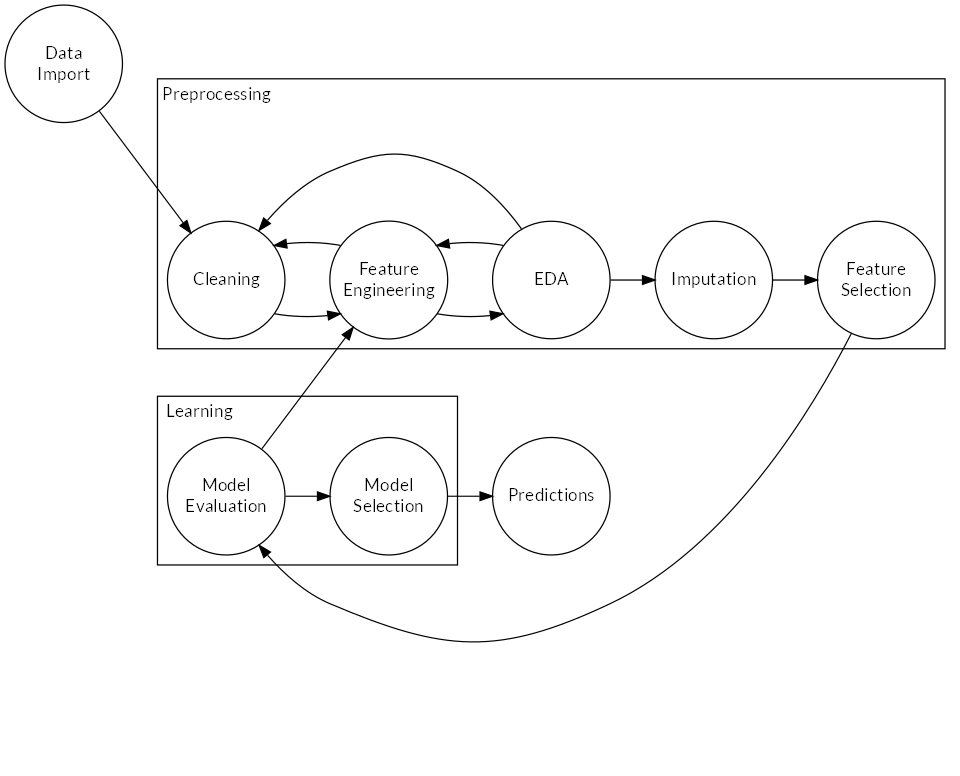
\includegraphics[width=0.8\linewidth]{figures/preprocessing/workflow} 

}

\caption{Implemented workflow. During import, data was type-cast to usable types. During preprocessing, input errors were corrected, binary features recoded, missing values correclty coded for each feature and categorical data processed manually where necessary. During feature engineering, redundant features were dropped, date features converted to time differences and geographical information acquired to visualize locations of examples.}\label{fig:workflow}
\end{figure}

\hypertarget{tools-used}{%
\section{Tools Used}\label{tools-used}}

The problem itself was solved using the python language with several established data-science packages. Except for the development of a helper packge, most programming was performed in interactive notebooks. The report was written in rmarkdown (see Allaire et al. (\protect\hyperlink{ref-allaire2016rmarkdown}{2016})) and rendered into several different output formats. All work was tracked in version control.

Some key tools are given below.

\hypertarget{jupyter-notebook}{%
\subsection{Jupyter Notebook}\label{jupyter-notebook}}

Following the principle of literate programming first proposed by Knuth (\protect\hyperlink{ref-knuth1984literate}{1984}), Jupyter by Kluyver et al. (\protect\hyperlink{ref-Kluyver:2016aa}{2016}) provides a client-server solution that enables interactive programming sessions in the browser. Blocks of code producing output including interactive plots can be mixed with formatted text. These notebooks can easily be shared with others or exported in various formats. The individual steps in the machine learning process outlined in Figure \ref{fig:workflow} were developed in several notebooks which are available online\footnote{see }, enabling the reproduction of the process.

For this thesis, jupyter notebooks were run in the cloud. The results were then exported and integrated in the report.

\hypertarget{pandas}{%
\subsection{Pandas}\label{pandas}}

The python package pandas by McKinney (\protect\hyperlink{ref-mckinney-proc-scipy-2010}{2010}) facilitates data loading, inspection and -manipulation. The package is very fast at transforming, filtering and selecting in big data sets.

\hypertarget{scikit-learn}{%
\subsection{Scikit-learn}\label{scikit-learn}}

The package scikit-learn by Pedregosa et al. (\protect\hyperlink{ref-scikit-learn}{2011}) is a self-contained toolset for machine learning purposes in python. Individual tasks in preprocessing, feature engineering and model training can be combined in pipelines. The pipelines ensure that the same transformation steps are applied to all data sets. The pipelines are first trained (fit) on the learning data and then applied (transform / predict) to the test data. A wide range of contribution and 3\textsuperscript{rd} party packages also implement scikit-learn's API so that they can be integrated.

\hypertarget{rmarkdown}{%
\subsection{Rmarkdown}\label{rmarkdown}}

The report was written in Rmarkdown. Analogous to a jupyter notebook, formatted text and code \emph{junks} can be integrated into one document. The R packages \texttt{knitr}, Xie (\protect\hyperlink{ref-xie2015}{2015}) and \texttt{bookdown}, Xie (\protect\hyperlink{ref-xie2016bookdown}{2016}) combined with a latex installation can then be employed to generate high-quality pdf documents and/or html versions.

\hypertarget{data-handling}{%
\section{Data Handling}\label{data-handling}}

The complete data is distributed pre-split into a learning and validation data set.

Preprocessing was performed on the learning data set.
After preprocessing, the learning data set was split 80/20 into training and validation sets (see Figure \ref{fig:data-splitting}). The training set was used to train different models while the validation set served to tune hyperparameters. The split was performed using a stratified sampling algorithm to preserve the target class frequencies.

The validation set was kept back until after model selection. The same preprocessing steps that were applied to the learning data set were then applied to the validation data set and the final prediction performed.

\begin{figure}

{\centering 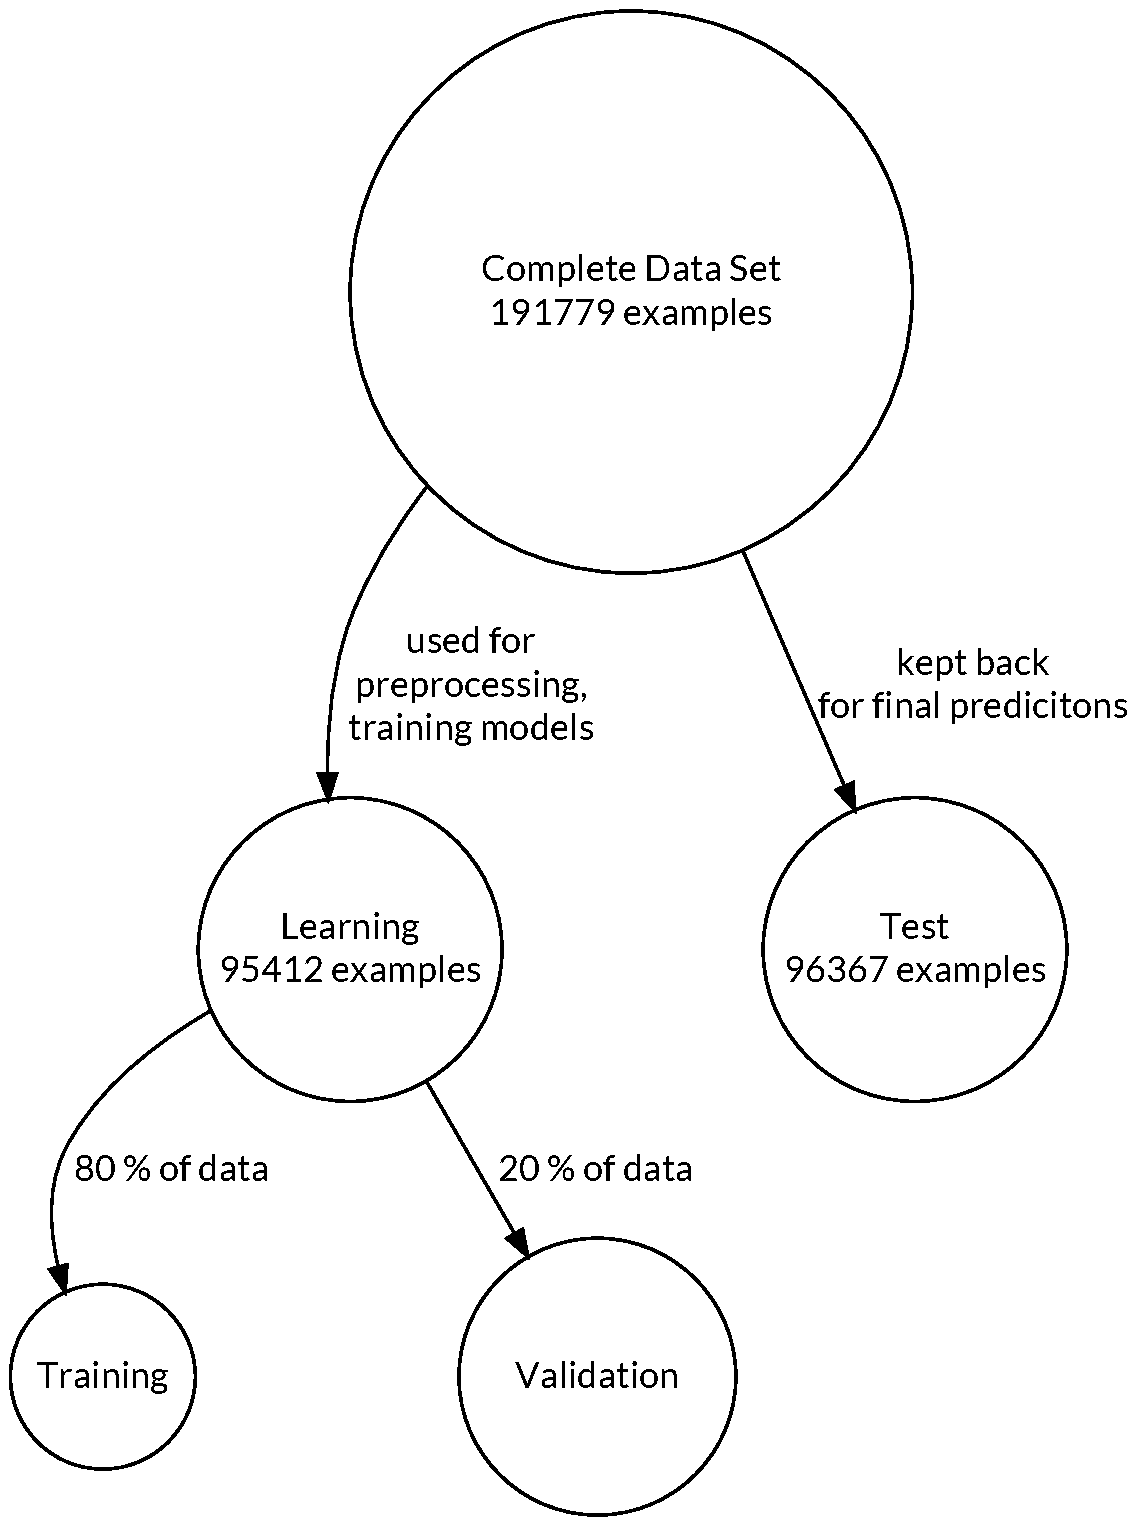
\includegraphics[width=0.5\linewidth]{figures/preprocessing/data-splitting} 

}

\caption{Data set use for training and predictions.}\label{fig:data-splitting}
\end{figure}

\hypertarget{data-preprocessing}{%
\section{Data Preprocessing}\label{data-preprocessing}}

To make data usable for learning algorithms, it generally has to be preprocessed. Preprocessing may encompass fixing input errors, coercing data to correct types, encoding categorical (string) data and dealing with missing values through imputation or removal. The result of this process is an all-numeric data set.

The necessary transformations were determined interactively in jupyter notebooks. Once finalized, the tranformations were implemented in the python package \texttt{kdd98}\footnote{see }. The package can be used to download and read in raw data and apply all transformations. Each transformation is enclosed in a class that implements scikit-learn's API for \texttt{BaseEstimator} and \texttt{TransformerMixin}, which allows for the transformations to be applied within a pipeline. Furthermore, the transformers can be trained and then persisted on disk for later application on other data.

The data set can be obtained at the following intermediate steps from \texttt{kdd98.data\_handler.KDD98DataProvider}:

\begin{itemize}
\tightlist
\item
  \textbf{raw}, as imported from csv using \texttt{pandas.read\_csv()}
\item
  \textbf{preprocessed}, input errors removed, correct data types for all features, missing at random (MAR) imputations applied
\item
  \textbf{numeric}, after feature engineering (encoded categories, date and zip code transformations)
\item
  \textbf{imputed}, with NaN-values replaced by modelled values
\item
  \textbf{all-relevant}, filtered down to a set of relevant features
\end{itemize}

\hypertarget{cleaning}{%
\subsection{Cleaning}\label{cleaning}}

The cleaning stage of preprocessing encompassed the following transformations:

\begin{itemize}
\tightlist
\item
  Removing `noise': Input errors, inconsistent encoding of binary / categorical features
\item
  Dropping constant and sparse (i.e.~those where only few examples have a value set) features
\item
  Imputation of values missing at random (MAR)
\end{itemize}

MAR values in the sense of Rubin (\protect\hyperlink{ref-rubin1976inference}{1976}) are missing conditionally on other features in the data. For example, there are three related features from the promotion and giving history: \emph{ADATE}, the date of mailing a promotion, \emph{RDATE}, the date of receiving a donation in response to the promotion and \emph{RAMOUNT}, the amount received. For missing \emph{RAMOUNT} values, we can check if \emph{RDATE} is non-missing. If \emph{RDATE} is missing, then the example most likely has not donated and we can set \emph{RAMOUNT} to zero. If, on the other hand, both date features have a value, \emph{RAMOUNT} is truly missing.

The transformations applied can be studied in the jupyter notebook \emph{1\_Preprocessing.ipynb}\footnote{see }.

\hypertarget{feature-engineering}{%
\subsection{Feature Engineering}\label{feature-engineering}}

During feature engineering, all non-numeric (i.e.~categorical) features were encoded into numeric values. Also, several features were transformed to better usable representations. Care was taken to keep the dimensionality of the data set as low as possible.

The result of this transformation step was an all-numeric data set usable for downstream learning. The transformations applied in feature engineering are described in detail in the jupyter notebook \emph{2\_Feature Engineering.ipynb}\footnote{see }.

\hypertarget{dates}{%
\subsubsection{Dates}\label{dates}}

All date features were transformed into time differences against a reference date according to Table \ref{tab:date-encoding}.

\begin{table}[!h]

\caption{\label{tab:date-encoding}Transformation of dates to time differences}
\centering
\begin{tabular}{>{\bfseries\raggedright\arraybackslash}p{3cm}>{\raggedright\arraybackslash}p{6cm}>{\raggedright\arraybackslash}p{6cm}l}
\toprule
  & Feature Explanation & Reference date & Unit\\
\midrule
DOB & Date of birth & 1997-06-01 (date of most recent campaign) & Years\\
RDATE & Month when donation was received & ADATE (sending date of the corresponding campaign) & Months\\
LASTDATE & Most recent donation prior to last campaign & 1997-06-01 & Months\\
MINRDATE & Date of smallest donation & 1997-06-01 & Months\\
MAXRDATE & Date of highest donation & 1997-06-01 & Months\\
\addlinespace
MAXADATE & Date of the most recent promotion received & 1997-06-01 & Months\\
\bottomrule
\end{tabular}
\end{table}

\hypertarget{zip-codes}{%
\subsubsection{Zip Codes}\label{zip-codes}}

U.S. zip codes were transformed into coordinates (latitude, longitude of the centroid for a given zip) using zip code tabulation data from United States Census Bureau (\protect\hyperlink{ref-census-gazet}{2018}). Several of the examples are army members, identifiable through their values in feature `STATE'. For these zip codes, no geographical data is available. These example's latitude and longitude were set to the coordinates of the pentagon, the U.S. department of defense.
The 2018 zip code tabulation data was missing several zip codes that existed in 1997, at the time of the campaign. These missing zip codes were looked up on the fly using a web service\footnote{\href{https://developer.here.com/products/geocoding-and-search}{HERE geocoding}}

\hypertarget{categorical-encoding}{%
\subsubsection{Categorical Encoding}\label{categorical-encoding}}

Categorical data was encoded using three different methods. For nominal features, the encoding method was chosen with respect to the number of levels in the categories. Nominal features with less than 10 levels were one-hot encoded. Those with more levels were binary-encoded. Ordinal features were consistently encoded to integer values.

A one-hot encoded feature with \(n\) levels is transformed into \(n\) new binary features, each feature representing one of the original levels. For each example, there can be at most one \texttt{true} value in these new features (denoting which category the example had in the original feature). If the original value was missing, all new features are set to missing.

Binary encoding first assigns an ordinal value to each category. These integer values are then binary encoded. For each binary digit, one new feature is created. Compared to one-hot encoding, the dimensionality increases less with this method.

As an example, the US states are represented by a categorical variable with 52 levels. While one-hot encoding would result in 52 new features, we can encode 52 values with only 5 binary

\hypertarget{imputation}{%
\subsection{Imputation}\label{imputation}}

As required by the cup documentation, missing values were imputed. Instead of choosing a simple approach like replacing with the feature's mean or median, a modelling approach was chosen. Package \texttt{fancyimpute} provides an iterative imputation algorithm for this purpose. Features are ordered by the fraction of missing values.

\hypertarget{feature-selection}{%
\subsection{Feature Selection}\label{feature-selection}}

One of the biggest caveats in machine learning is the infamous ``Curse of Dimensionality'' coined by Bellman, Corporation, and Collection (\protect\hyperlink{ref-bellman1957dynamic}{1957}). The curse comes from the fact that with an increasing number of dimensions, the required number of examples grows exponentially. In the area of machine learning, high dimensionality in short frequently leads to an overfitting of the training data, meaning that the generalisation error is unacceptably big (see Goodfellow, Bengio, and Courville (\protect\hyperlink{ref-Goodfellow-et-al-2016}{2016})).

It is therefore beneficial to reducde the data set dimensionality while preserving as much relevant information as possible. A method to deal with the problem is called boruta, introduced by Kursa, Rudnicki, and others (\protect\hyperlink{ref-kursa2010boruta}{2010}). It works sequentially and removes features found to be less relevant at each iteration. By doing so, it solves the so-called all-relevant feature problem.
The algorithm is acutally a wrapper function around a random forest classifier. A random forest classifier is fast, can usually be run without parameters and returns an importance measure for each feature.

In short, the alogrithm works as follows:

\begin{enumerate}
\def\labelenumi{\arabic{enumi}.}
\tightlist
\item
  The input matrix \(\mathbf{X}\) of dimension \(n\text{ x }p\) is extended with \(p\) so-called \emph{shadow features}. The shadow features are permuted copies of the features in \(\mathbf{X}\). They are therefore decorrelated with the target.
\item
  On the resulting matrix \(\mathbf{X^*}\), a random forest classifier is trained and the Z-scores (\(\frac{\bar{loss}}{sd}\)) for each of the \(2p\) features calculated.
\item
  The highest Z-score among the shadow features \(MZSA\) is determined.
\item
  All original features are compared against \(MZSA\) and those features with a higher score selected as important.
\item
  With the remaining features, a two-sided test for equality of the Z-scores with \(MZSA\) is performed and all features with significantly lower score are deemed unimportant.
\item
  All shadow copies are removed, go to step 1.
\end{enumerate}

The algorithm terminates when all attributes are marked as either important or not important or when the maximum number of iterations is reached.

For this thesis, a python implementation\footnote{see \href{https://github.com/scikit-learn-contrib/boruta_py}{scikit-learn-contrib/boruta\_py}} was used. In effect, it is a port of the original R package by Kursa, Rudnicki, and others (\protect\hyperlink{ref-kursa2010boruta}{2010}) which plugs into scikit-learn.

\hypertarget{model-evaluation}{%
\section{Model Evaluation}\label{model-evaluation}}

For this thesis, several different algorithms were studied.

\hypertarget{considered-algorithms}{%
\subsection{Considered Algorithms}\label{considered-algorithms}}

\hypertarget{gradient-boosting-machine}{%
\subsubsection{Gradient Boosting Machine}\label{gradient-boosting-machine}}

Boosting is a method that can be applied to any learning algorithm. It was introduced by Freund and Schapire (\protect\hyperlink{ref-freund1997decision}{1997}) in the form of the algorithm AdaBoost.M1, intended for classification problems. The main idea behind boosting is to train a set of weak classifiers which are only slightly better than a random decision. The predictions of the individual weak classifiers are then combined into a majority vote.

Gradient boosting extends on this idea.

In the scope of this thesis, the package \texttt{XGBoost} by Chen and Guestrin (\protect\hyperlink{ref-chen2016xgboost}{2016}) was used. Assume we have a data set with \(n\) examples and \(m\) features: \(D = \{\{\mathbf{x_i}, y_i\}\} ( |D| = n, \mathbf{x_i} \in \mathbb{R}^m, y_i \in \mathbb{R})\). The implementation uses a tree ensemble using \(K\) additive functions (regression trees) to predict the outcome for an example in the data.

\begin{equation}
\hat{y}_i = \phi(\mathbf{x_i}) = \sum_{k=1}^K f_k(\mathbf{x_i}), f_k \in F
\label{eq:gbm-ensemble}
\end{equation}

where \(F = \{f(\mathbf{x}) = w_{q(x)}\} (q: \mathbb{R}^m \rightarrow T, w \in \mathbb{R}^T)\) is the space of regression trees. \(T\) is the number of leaves in a tree, \(q\) is the structure of each tree, mapping an example to the corresponding leaf index. Each tree \(f_k\) has an independent structure \(q\) and weights \(w\) at the terminal leafs. An example is classified on each tree in \(F\) and the weights of the corresponding leafs are summed up to calculate the final prediciton.

For learning the functions in \(F\), the following loss function is minimized:

\begin{equation}
L(\phi) = \sum_{i=1}^n l(\hat{y}_i, y_i) + \sum_k^K \Omega(f_k)
\label{eq:gbm-loss}
\end{equation}

Here, \(l\) is a differentiable, convex loss function that measures the difference between predictions and true values. Since \(l\) is convex, we are guaranteed to find a global minimum. \(\Omega(f) = \gamma T + \frac{1}{2}\lambda||w||^2\) is a penalty on the complexity of the trees to counter over-fitting.

\hypertarget{random-forest}{%
\subsubsection{Random Forest}\label{random-forest}}

\hypertarget{support-vector-machine}{%
\subsubsection{Support Vector Machine}\label{support-vector-machine}}

\hypertarget{neural-network}{%
\subsubsection{Neural Network}\label{neural-network}}

\hypertarget{glm-net}{%
\subsubsection{GLM Net}\label{glm-net}}

\hypertarget{performance-metrics}{%
\subsection{Performance Metrics}\label{performance-metrics}}

For classification problems, the confusion matrix (see Table \ref{tab:conf-matrix-def}) helps in constructing several performance measures. If we predict an event correctly, it is a \emph{true positive} (TP), predicting an event if there is none, it is a \emph{false positive} (FP). A \emph{false negative} (FN) occures when predicting no event when there was one and a \emph{true negative} (TN) occurs when no event was predicted correctly.

\begin{table}[!h]

\caption{\label{tab:conf-matrix-def}Definition of the confusion matrix}
\centering
\begin{tabular}{>{\bfseries}l>{\bfseries}lll}
\toprule
\multicolumn{2}{c}{ } & \multicolumn{2}{c}{True value} \\
\cmidrule(l{3pt}r{3pt}){3-4}
  &   & Event & No Event\\
\midrule
 & Event & TP & FP\\
\cmidrule{2-4}
\multirow{-2}{*}{\raggedright\arraybackslash Predicted} & No Event & FN & TN\\
\bottomrule
\end{tabular}
\end{table}

\begin{verbatim}
                 Event No Event
\end{verbatim}

1 Predicted Event TP FP
2 Predicted No Event FN TN

From the confusion matrix, several metrics can be deduced. The definitions of some often-used metrics are given below:

\begin{align*}
\text{Accuracy} &= \frac{TP + TN}{TP + FP + FN + TN} \\
\text{Sensitivity} &= \frac{TP}{TP + FN} \\
\text{Specificity} &= \frac{TN}{TN + FP} \\
\text{Precision} &= \frac{TP}{TP + FP} \\
\text{F1 score} &= \frac{2TP}{2TP+FP+FN}
\end{align*}

In literature the following synonyms are found:

\begin{itemize}
\tightlist
\item
  Precision: Positive predictive value (PPV)
\item
  Sensitivity: Recall, True positive rate (TPR), hit rate
\item
  Specificity: Selectivity, True negative rate (TNR)
\end{itemize}

It is evident that sensitivity measures the proportion of the predicted events from all events present.

Analogous, specificity measures the proportion of correctly predicted no events from all no events present.

\hypertarget{data}{%
\chapter{Data}\label{data}}

The data at hand is a subset of the roughly 3.5 million members of the organization who were targeted by a campaign in 1997. All donors who were contacted in this campaign have donated at least once to the organisation in the past.

The dataset, which is freely available online\footnote{See \href{https://archive.ics.uci.edu/ml/datasets/KDD+Cup+1998+Data}{UCI Machine Learning Repository: KDD Cup 1998 Data}} contains information on a subset of the turnout of a direct mailing addressed to 3.5 million members in the scope of a fundraising campaign that was conducted in 1997. The dataset contains all donors with a \emph{lapsed} donation status, meaning their last donation was made between 13 and 24 months prior to the 1997 campaign.

The data is provided in two sets, of which one is intended for learning, the other for validation.

In the following section, the learning data set will be characterized. All preprocessing and feature engineering steps were also applied identically to the validation data set.

\hypertarget{raw-data-import}{%
\section{Raw data import}\label{raw-data-import}}

The import through \texttt{pandas.read\_csv()} was facilitated by providing per-feature specifications for missing values and explicit type casting for nominal categories. Ordinal categories, dates and features with binary values were cast to the type string (Object).

The dimension of the input data is 95412 examples by 481 features. Of the features, two are the targets and one was used as the index, leaving 478 explanatory features.

The dataset structure after import into a \texttt{pandas.DataFrame} object is presented in Table \ref{tab:data-desc}.
This corresponds to the \emph{raw} stage in preprocessing.

\begin{table}[!h]

\caption{\label{tab:data-desc}Data types after import of raw csv data}
\centering
\begin{tabular}{l>{\raggedright\arraybackslash}p{6cm}l}
\toprule
  & Data content & Number of features\\
\midrule
Integer & Discrete features, no missing values & 297\\
Float & Continuous features and discrete features with missing values & 49\\
Categorical & Nominal and ordinal features & 24\\
Object & Features with alphanumeric values & 110\\
Total &  & 480\\
\bottomrule
\end{tabular}
\end{table}

\hypertarget{cleaning-preprocessing}{%
\section{Cleaning \& Preprocessing}\label{cleaning-preprocessing}}

\hypertarget{date-features}{%
\subsection{Date features}\label{date-features}}

There were 53 date features specified in the documentation. The specified format for these features is `yymm', the two-digit year followed by the two-digit month.

\begin{figure}

{\centering 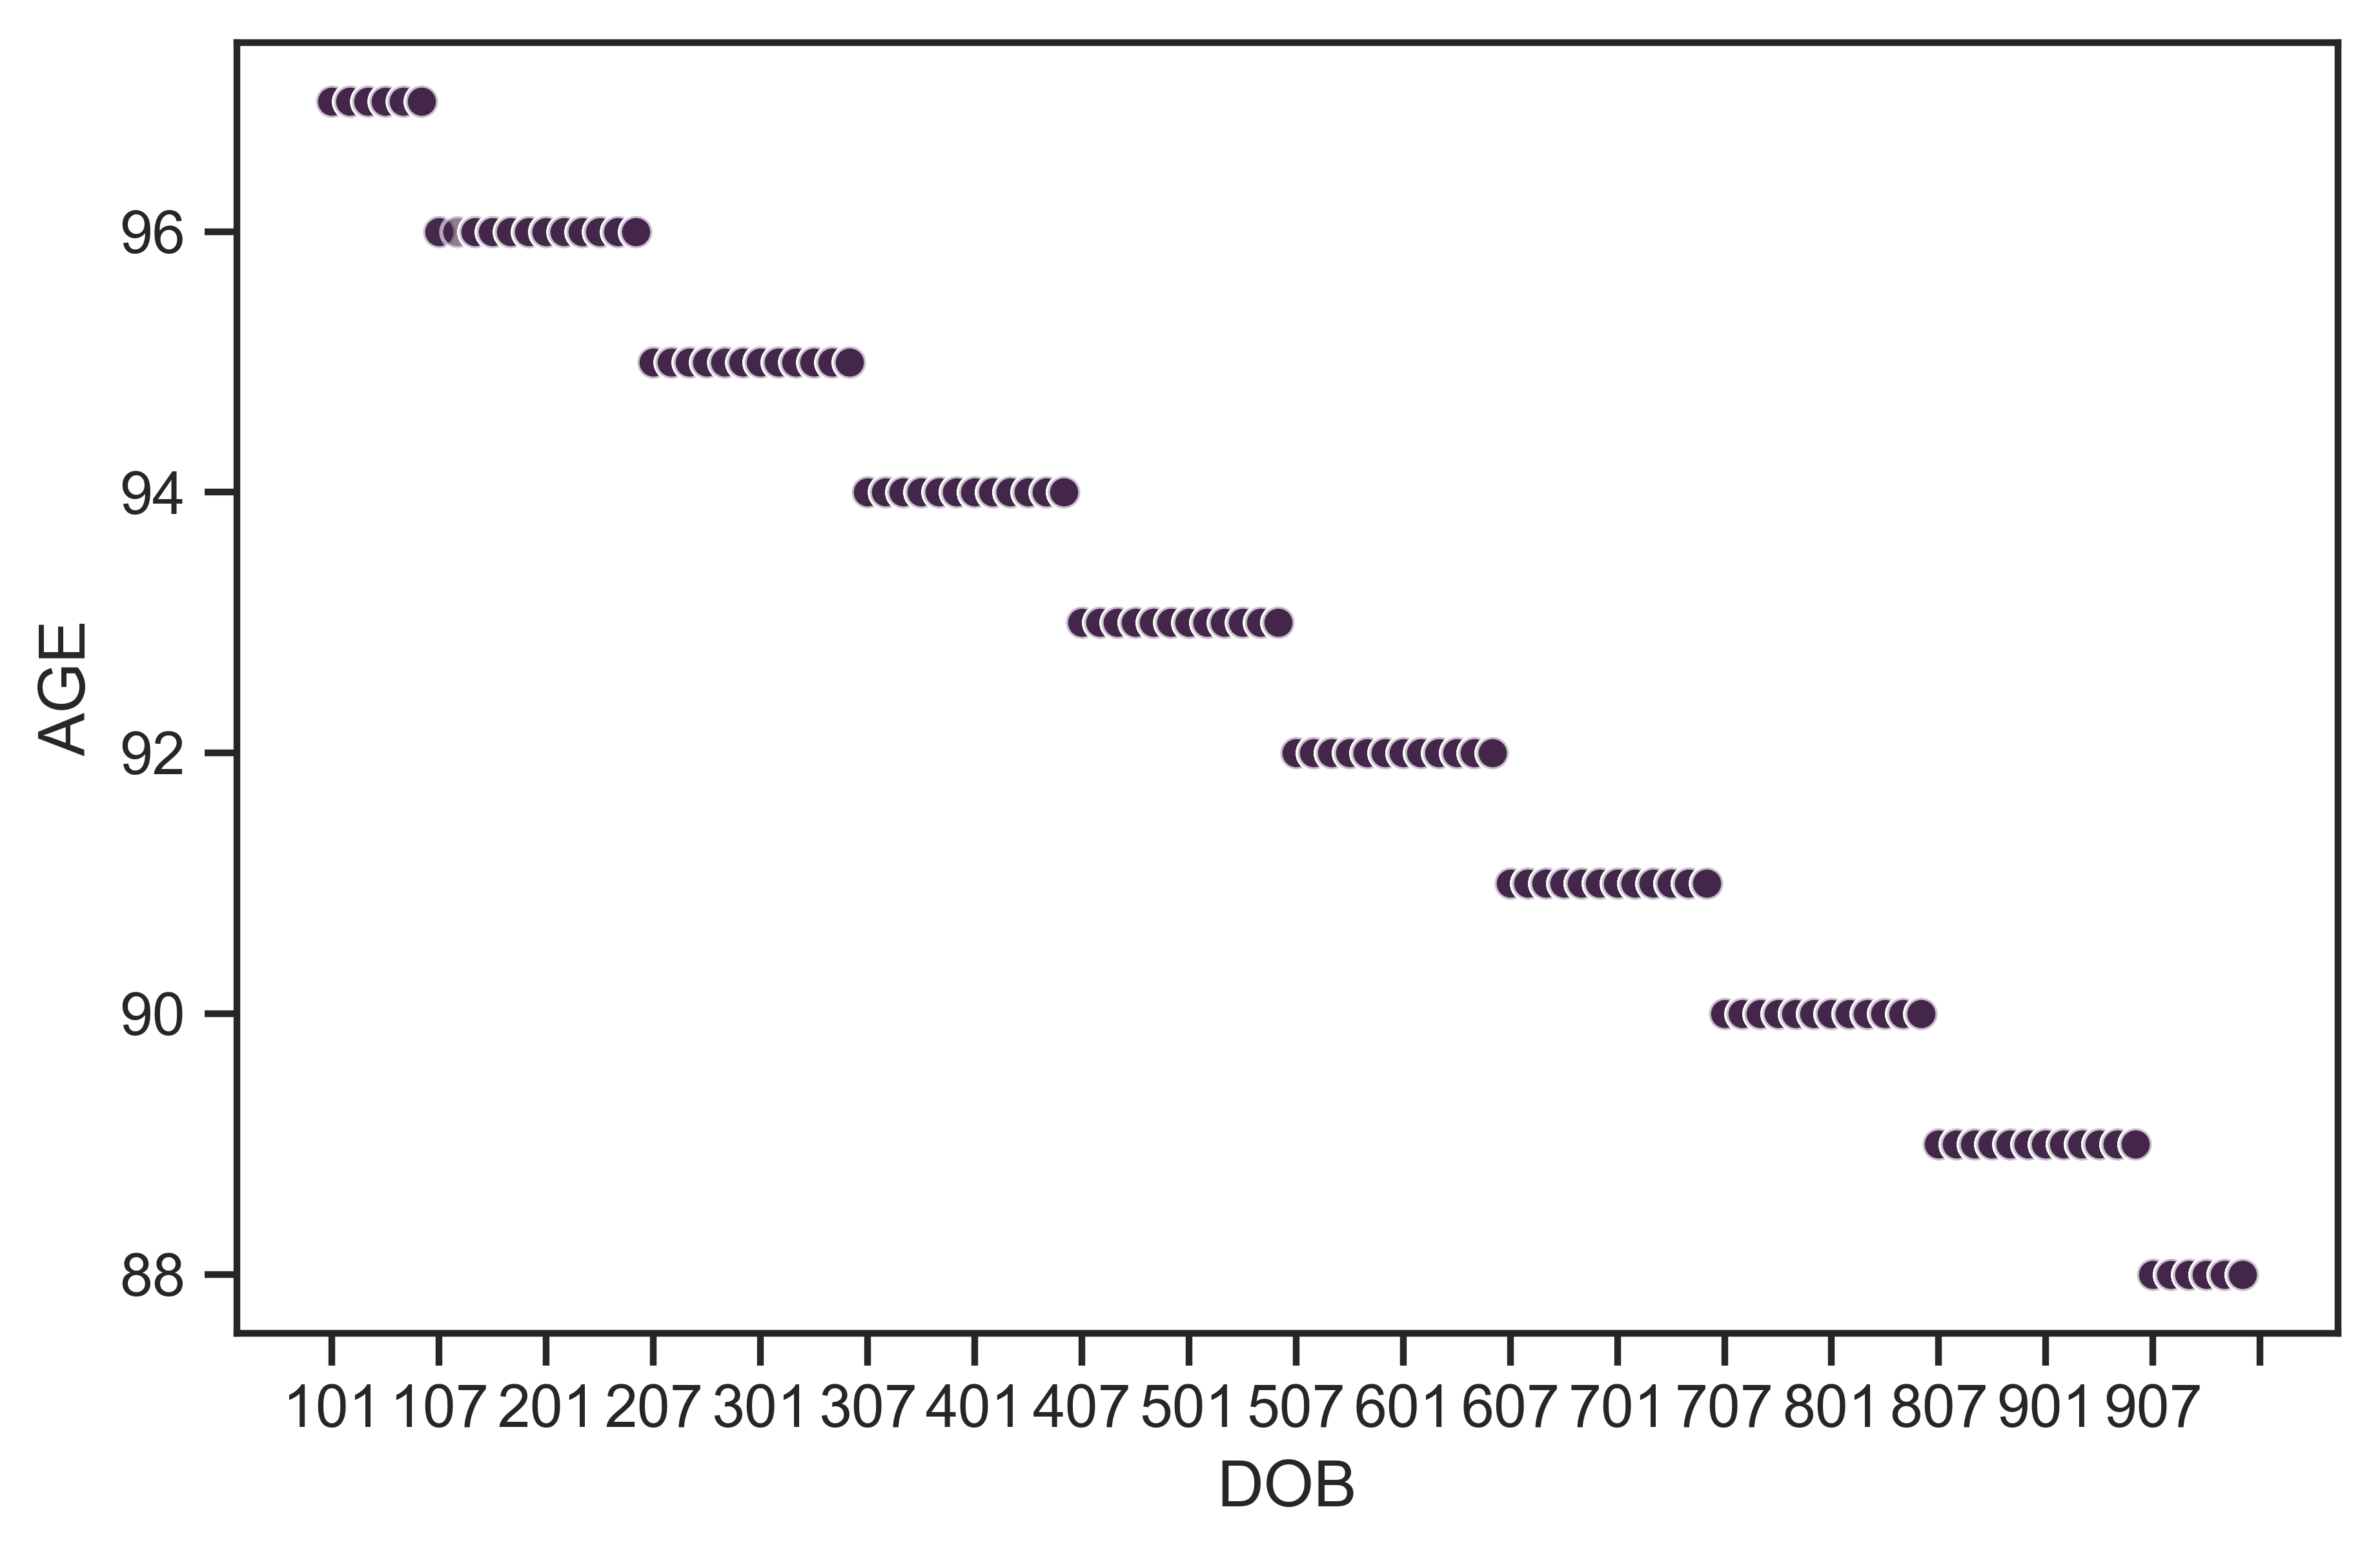
\includegraphics[width=0.7\linewidth]{./figures/date-cleaning-1} 

}

\caption{Values for date of birth (DOB) with one missing digit versus age. We observe jumps in July of each year, this is because the reference date for age is 1997-06-01. By looking at the ages, it is evident that these values indeed lack a leading zero to put them in the correct decade.}\label{fig:date-cleaning}
\end{figure}

Several values in the feature DOB (date of birth) are only three digits long. Comparing these values with the corresponding example's values for feature AGE shows that, considering the reference date of June 1997, it is very likely that the 3-digit DOB's are lacking a leading zero (see Figure \ref{fig:date-cleaning}).

All these values were therefore prepended by a zero.

\hypertarget{further-sanitizations}{%
\subsection{Further sanitizations}\label{further-sanitizations}}

Several features needed recoding and sanitizing. Information in the data set documentation was used to determine necessary transformations. The transformations are shown in \ref{tab:sanitize}.

\begin{table}[!h]

\caption{\label{tab:sanitize}Overview of trivial data transformations applied.}
\centering
\begin{tabular}{l>{\raggedright\arraybackslash}p{4cm}>{\raggedright\arraybackslash}p{4cm}>{\raggedright\arraybackslash}p{4cm}}
\toprule
  & Feature explanation & Operation & Reason\\
\midrule
ZIP & U.S. zip code & Remove trailing hyphen & A hyphen after a 5-digit zip most likely stems from incomplete 'ZIP+4' codes\textasciicircum{}[see (USPS: ZIP+4 Code)[https://about.usps.com/publications/pub100/pub100\_044.htm]].\\
MDMAUD\_* & Major donor matrix features & Replace X with NaN & Encode NaN as specified by the data set documentation.\\
TARGET\_B & Binary target indicating whether an example has donated or not. & Set to 1 when TARGET\_D is \$
ew\$ 0 & When a dollar amount (TARGET\_D) was donated, the binary indicator target has to be 1.\\
RFA\_* & Multi-byte categorical. Recency, Frequency, Amount. & Set to NaN if length is \$
eq\$ 3 & The values in these features have to be of length 3, each byte is one categorical.\\
NOEXCH & NOEXCH: Do not exchange address flag & Recode X to 1 & Both X and 1 mean `True`\\
\addlinespace
RAMNT\_* & RAMNT\_*: Amount donated for a certain campaign. & Set to NaN if corresponding RDATE\_* (date of donation reception) is not missing, else set to zero. & Avoid NaN values if possible.\\
\bottomrule
\end{tabular}
\end{table}

\hypertarget{binary-features}{%
\subsection{Binary Features}\label{binary-features}}

There are several codings for the different binary features present in the data set. All were recoded to \emph{1} / \emph{0} with missing data coded as not a number (NaN). The recoding was done through a custom \texttt{Transformer} class (see Appendix \ref{appendix-transformers}) derived from scikit-learn's \texttt{TransformerMixin}.

Table (\ref{tab:binary-recode}) shows the original coding of the 29 binary features in the raw data set. There are two classes of binary features that have blanks as the \emph{False} value. Even though the data set documentation states that blanks should be treated as missing values, in these two classes blanks were interpreted as \emph{False}. For the remaining binary features, blanks were interpreted as missing and coded as \texttt{NaN}.

The feature \emph{NOEXCH} had both \texttt{X} and \texttt{1} for True in the data. This was fixed by replacing all occurrences of \texttt{X} by \texttt{1}.

\begin{table}[!h]

\caption{\label{tab:binary-recode}Original coding of binary features.}
\centering
\begin{tabular}{ll>{\raggedright\arraybackslash}p{10cm}}
\toprule
True & False & Features\\
\midrule
X & blank & PEPSTRFL, MAJOR, RECINHSE, RECP3, RECPGVG, RECSWEEP\\
Y & N & COLLECT1, VETERANS, BIBLE, CATLG, HOMEE, PETS, CDPLAY, STEREO,
      PCOWNERS, PHOTO, CRAFTS, FISHER, GARDENIN,  BOATS, WALKER, KIDSTUFF,
      CARDS, PLATES\\
1 & 0 & NOEXCH, HPHONE\_D, TARGET\_B\\
E & I & AGEFLAG\\
H & U & HOMEOWNR\\
\addlinespace
B & blank & MAILCODE\\
\bottomrule
\end{tabular}
\end{table}

\hypertarget{multi-byte-categorical-features}{%
\subsection{Multi-byte Categorical Features}\label{multi-byte-categorical-features}}

Several features combine related information into bytewise codes. These codes were split into individual features. A custom child class of \texttt{scikit-learn.TransformerMixin} was written for this purpose (see Appendix \ref{appendix-transformers}).

The donation history contains recency / frequency / amount (RFA) features for each previous mailing. The dataset already contained one mailing (number 2) where this code was split into individual features. The remaining RFA codes were split also.

\hypertarget{ordinal-features}{%
\subsubsection{Ordinal Features}\label{ordinal-features}}

Ordinal features were recoded using a custom child classes of \texttt{scikit-learn.TransformerMixin} (see Appendix \ref{appendix-transformers}).

\hypertarget{missing-values}{%
\subsection{Missing Values}\label{missing-values}}

Missing values were imputed using a k-Neaerest Neighbors (kNN) algorithm provided in the python package \texttt{missing\_py} Troyanskaya et al. (\protect\hyperlink{ref-troyanskaya2001missing}{2001}). For each example with a missing value in a specific feature, \(k=3\) nearest neighbors that have a value for the feature are searched for and the missing value imputed with the metric \emph{distance}.

\hypertarget{exploratory-data-analysis}{%
\section{Exploratory Data Analysis}\label{exploratory-data-analysis}}

The detailed analysis can be studied online in the corresponding jupyter notebook\footnote{\href{https://github.com/datarian/master-thesis-code/blob/development/notebooks/eda.ipynb}{KDD-CUP98: EDA notebook}}. The findings are shown here.

\hypertarget{general-structure}{%
\subsection{General structure}\label{general-structure}}

The data set is provided pre-cut into a learning and validation set with 95412 and 96367 examples. The features are identical between the two except for the target that has been stripped from the validation set.

There are four main sources of information that make up the data:

\begin{itemize}
\tightlist
\item
  Internal member database (index, personal particulars, several member status features): 85 features
\item
  US census 1990: 286 features
\item
  Promotion history file: 97 features on promotions received up until the current mailing and response patterns to these promotions
\item
  Giving history file: 13 features, summary statistics giving maximum and minimum amount donated and dates of donations
\end{itemize}

In total, there are 479 features plus two \protect\hyperlink{targets}{targets}.

\hypertarget{correlations}{%
\subsection{Correlations}\label{correlations}}

\hypertarget{skewness}{%
\subsection{Skewness}\label{skewness}}

Most of the data is skewed. This is an important finding as the data will have to be transformed for learning algorithms that do not perform well for this kind of data.

Figure \ref{fig:skew-all} gives an abstract idea of the skewness of (numerical) features. It was measured with \texttt{pandas.skew()}, which uses the Fisher-Pearson standardized moment coefficient \(G_1 = \frac{\sqrt{n(n-1)}}{n-2}\frac{1}{n}\frac{\sum_{i=1}^n (x_i-\bar{x})^3}{s^3}\). Here, the term in the denominator is the sample standard deviation.

\textbackslash{}begin\{figure\}

\{\centering 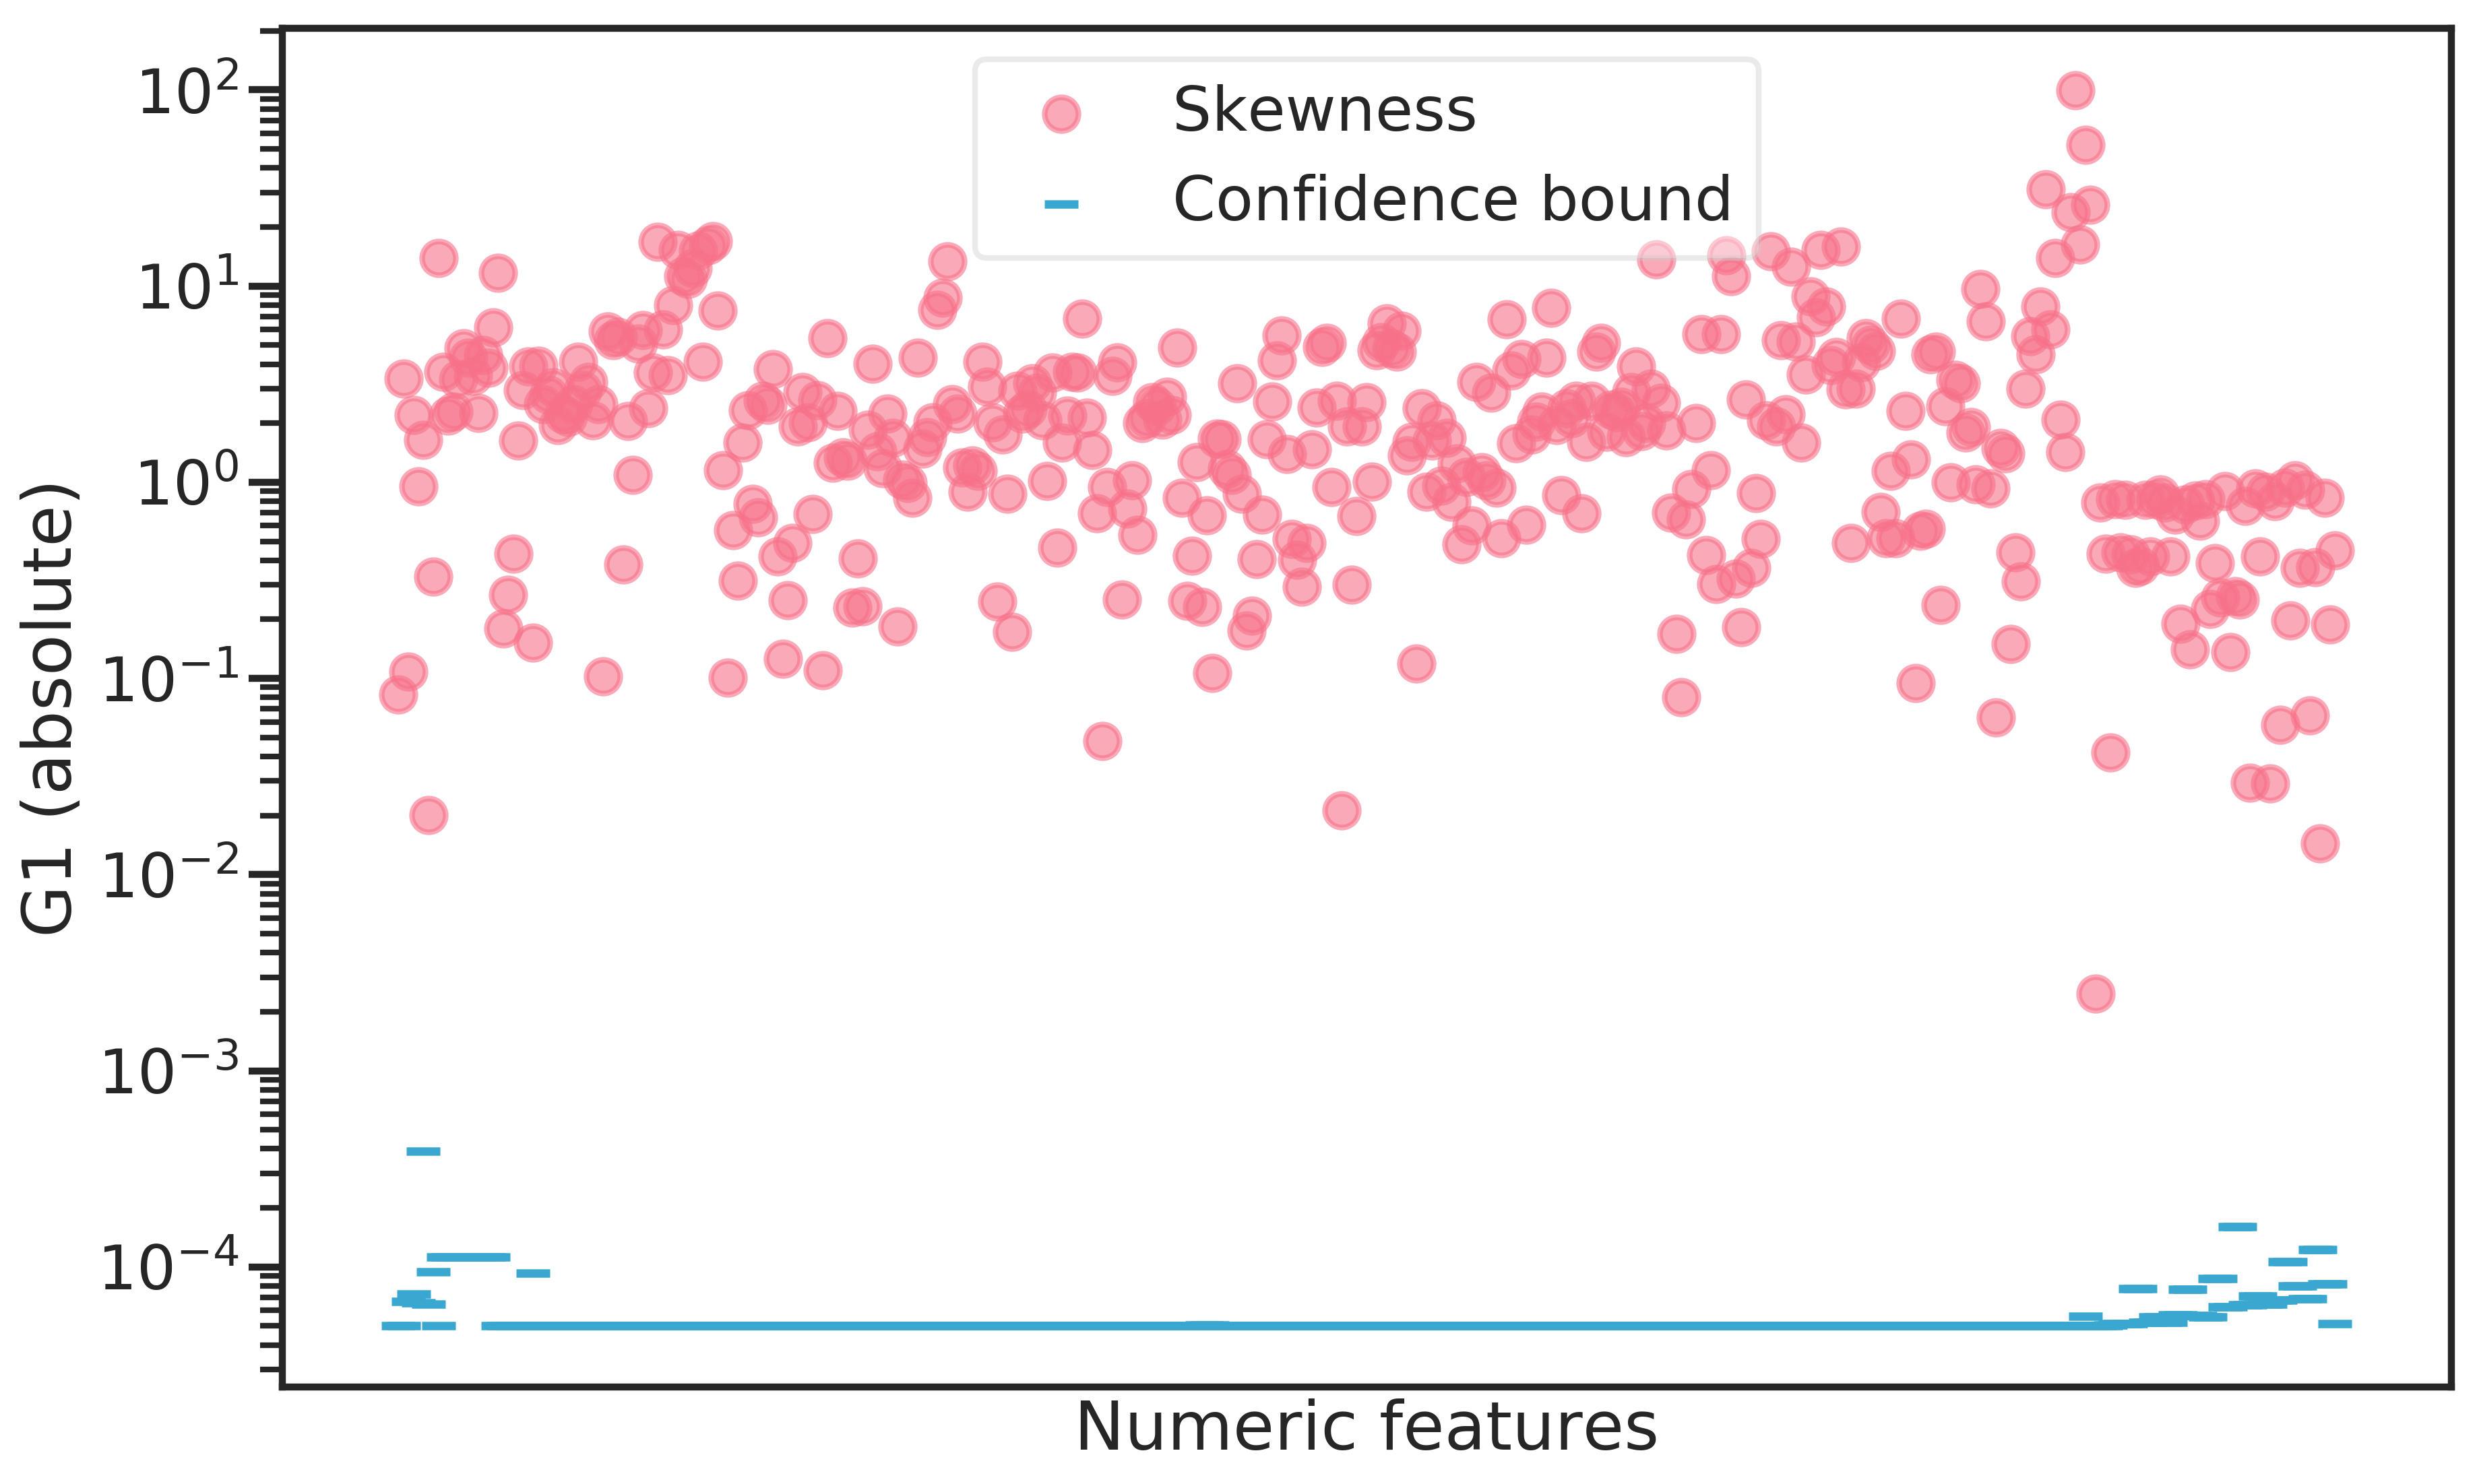
\includegraphics[width=0.7\linewidth]{figures/eda/skewness-numeric-features}

\}

\textbackslash{}caption\{Absolute values of the Fisher-Pearson standardized moment coefficient (G1) for all numeric features contained in the dataset. The confidence bound indicates the \(\alpha\) = 5 \% bound for the skewness of a symmetric distribution for any given feature. It is evident that no feature passes.\}\label{fig:skew-all}
\textbackslash{}end\{figure\}

The confidence bound in Figure \ref{fig:skew-all} gives the \(\alpha=5 \%\) bound for a normal distribution. Evidently, no feature was found to be strictly normally distributed, although several features show quite symmetric distributions (see Figure \ref{fig:least-skewed}). These symmetric distributions resemble normal or uniform distributions.

\begin{figure}

{\centering 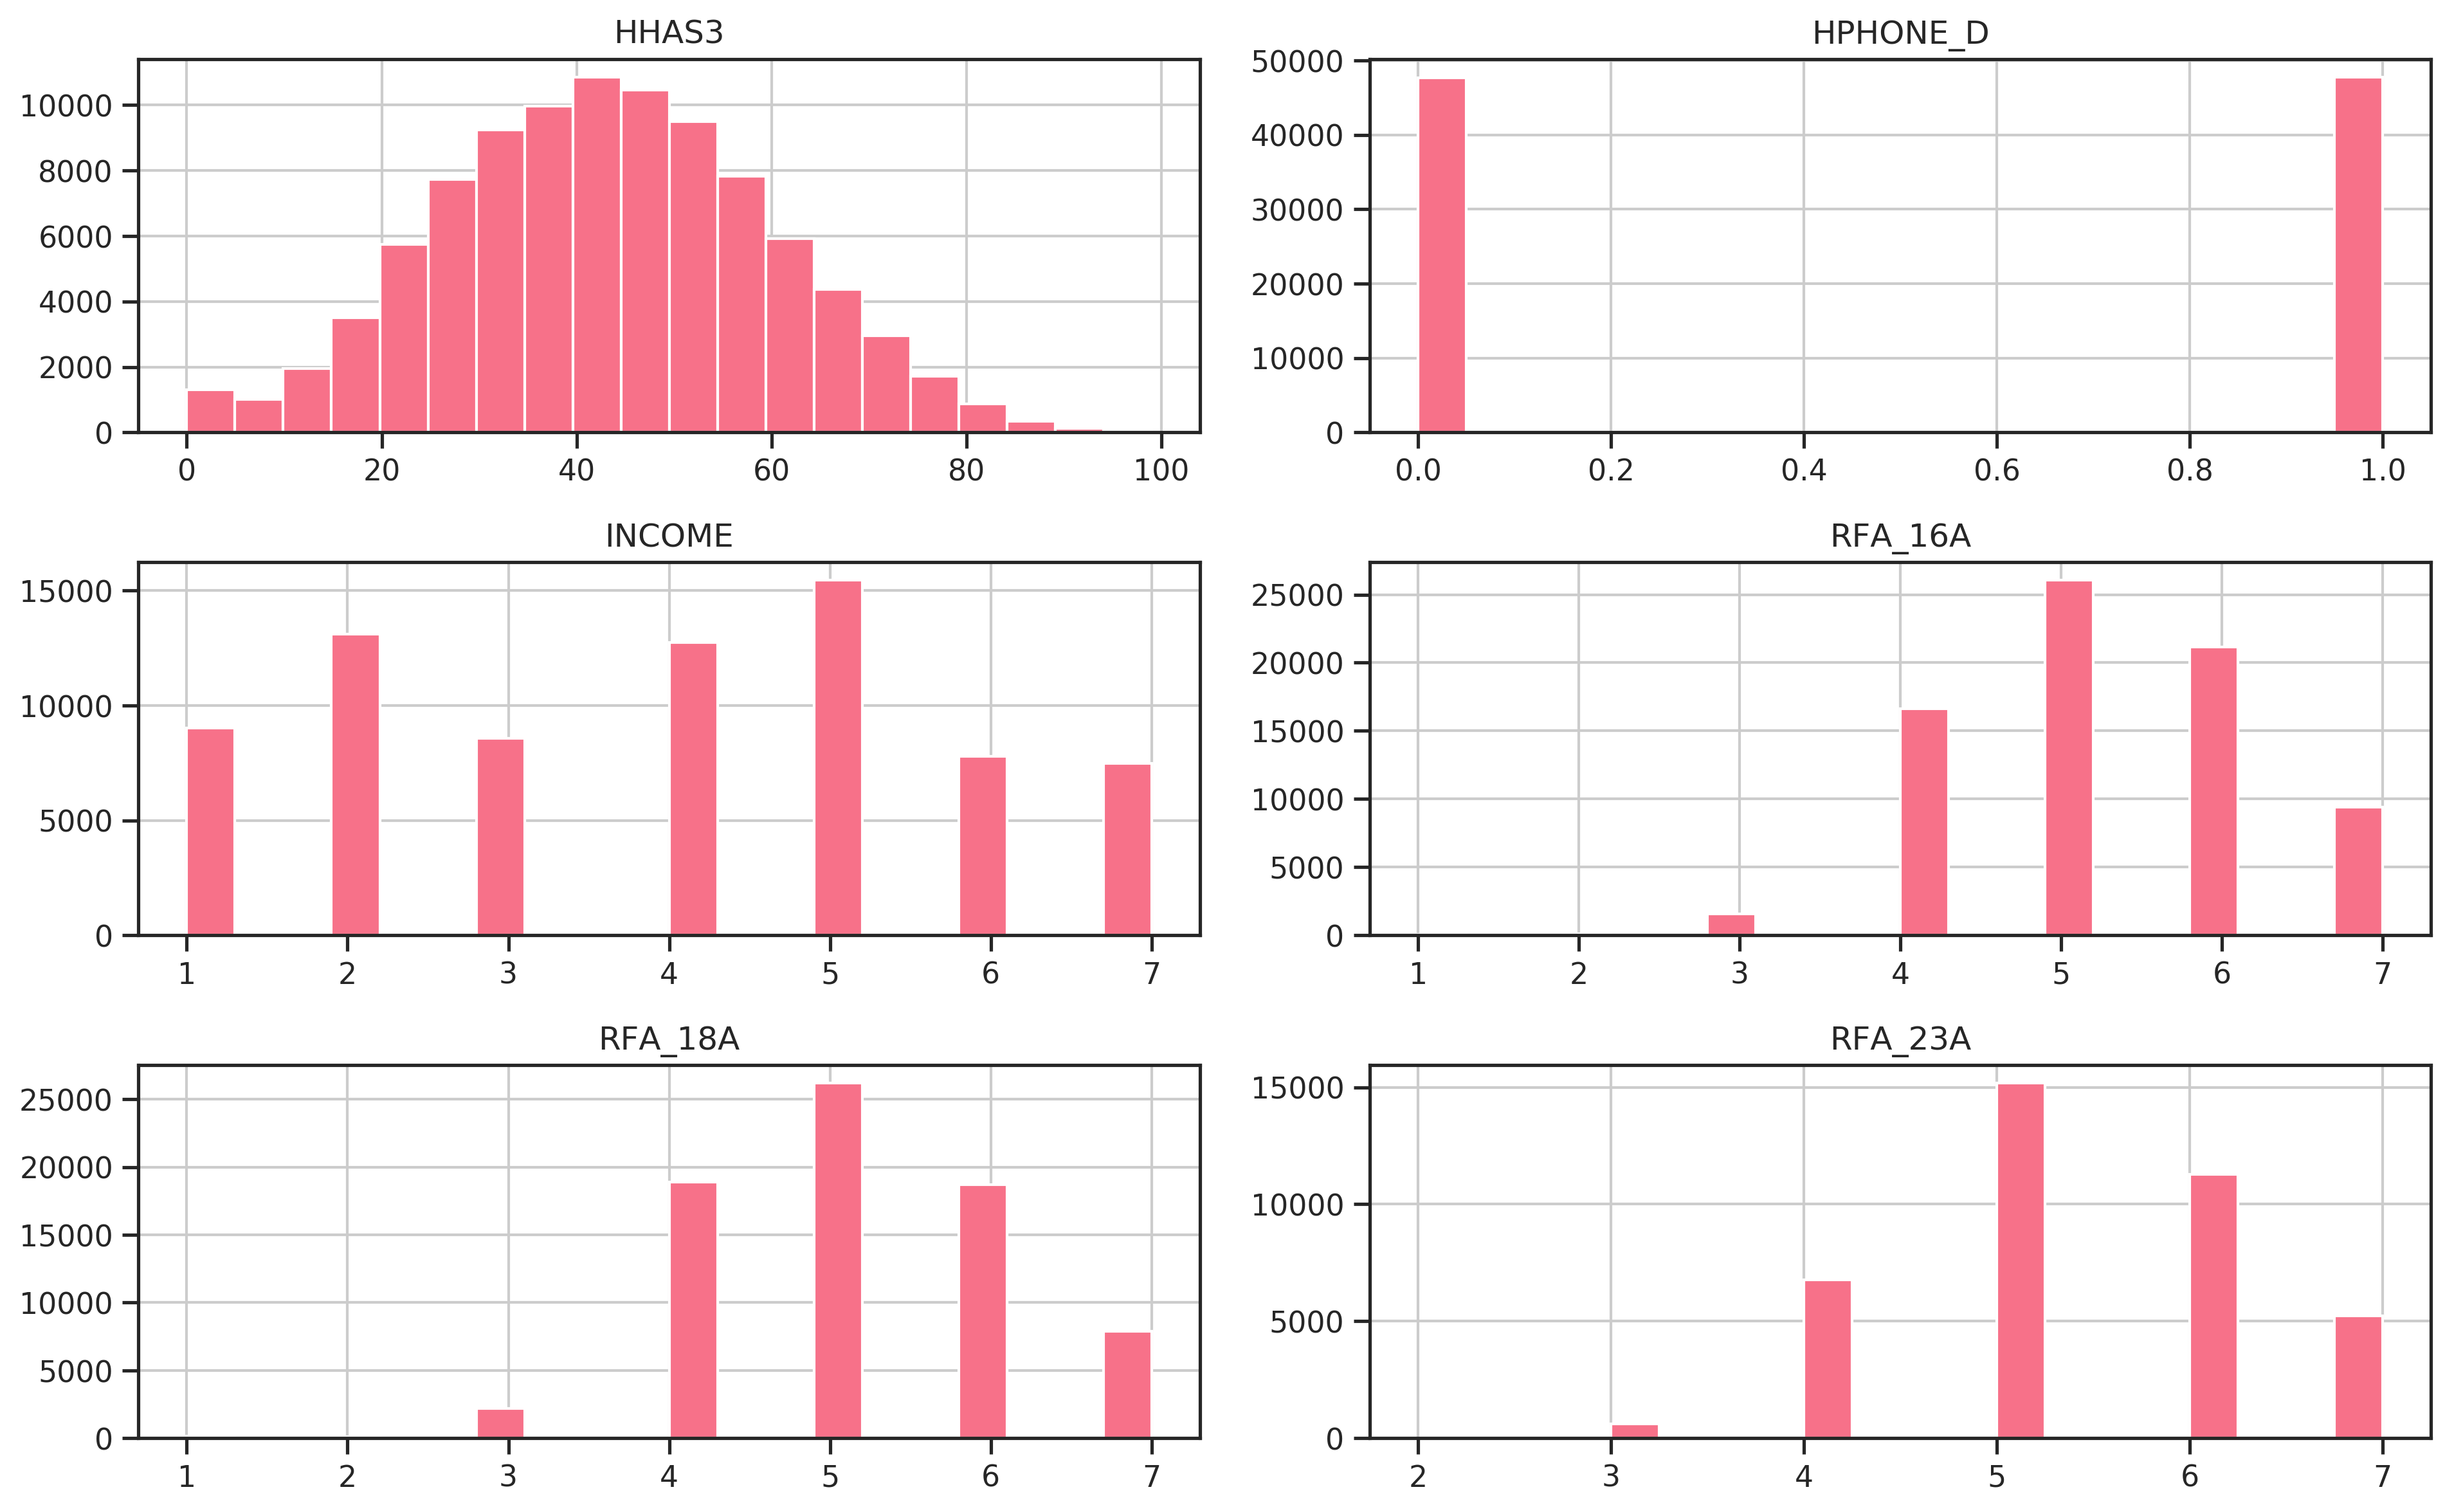
\includegraphics[width=0.7\linewidth]{figures/eda/least-skewed} 

}

\caption{The 9 least skewed features. Skewness metric: adjusted Fisher-Pearson standardized moment coefficient.}\label{fig:least-skewed}
\end{figure}

Looking at the most skewed features (see Figure \ref{fig:most-skewed}), we see heavily right-skewed distributions.

\begin{figure}

{\centering 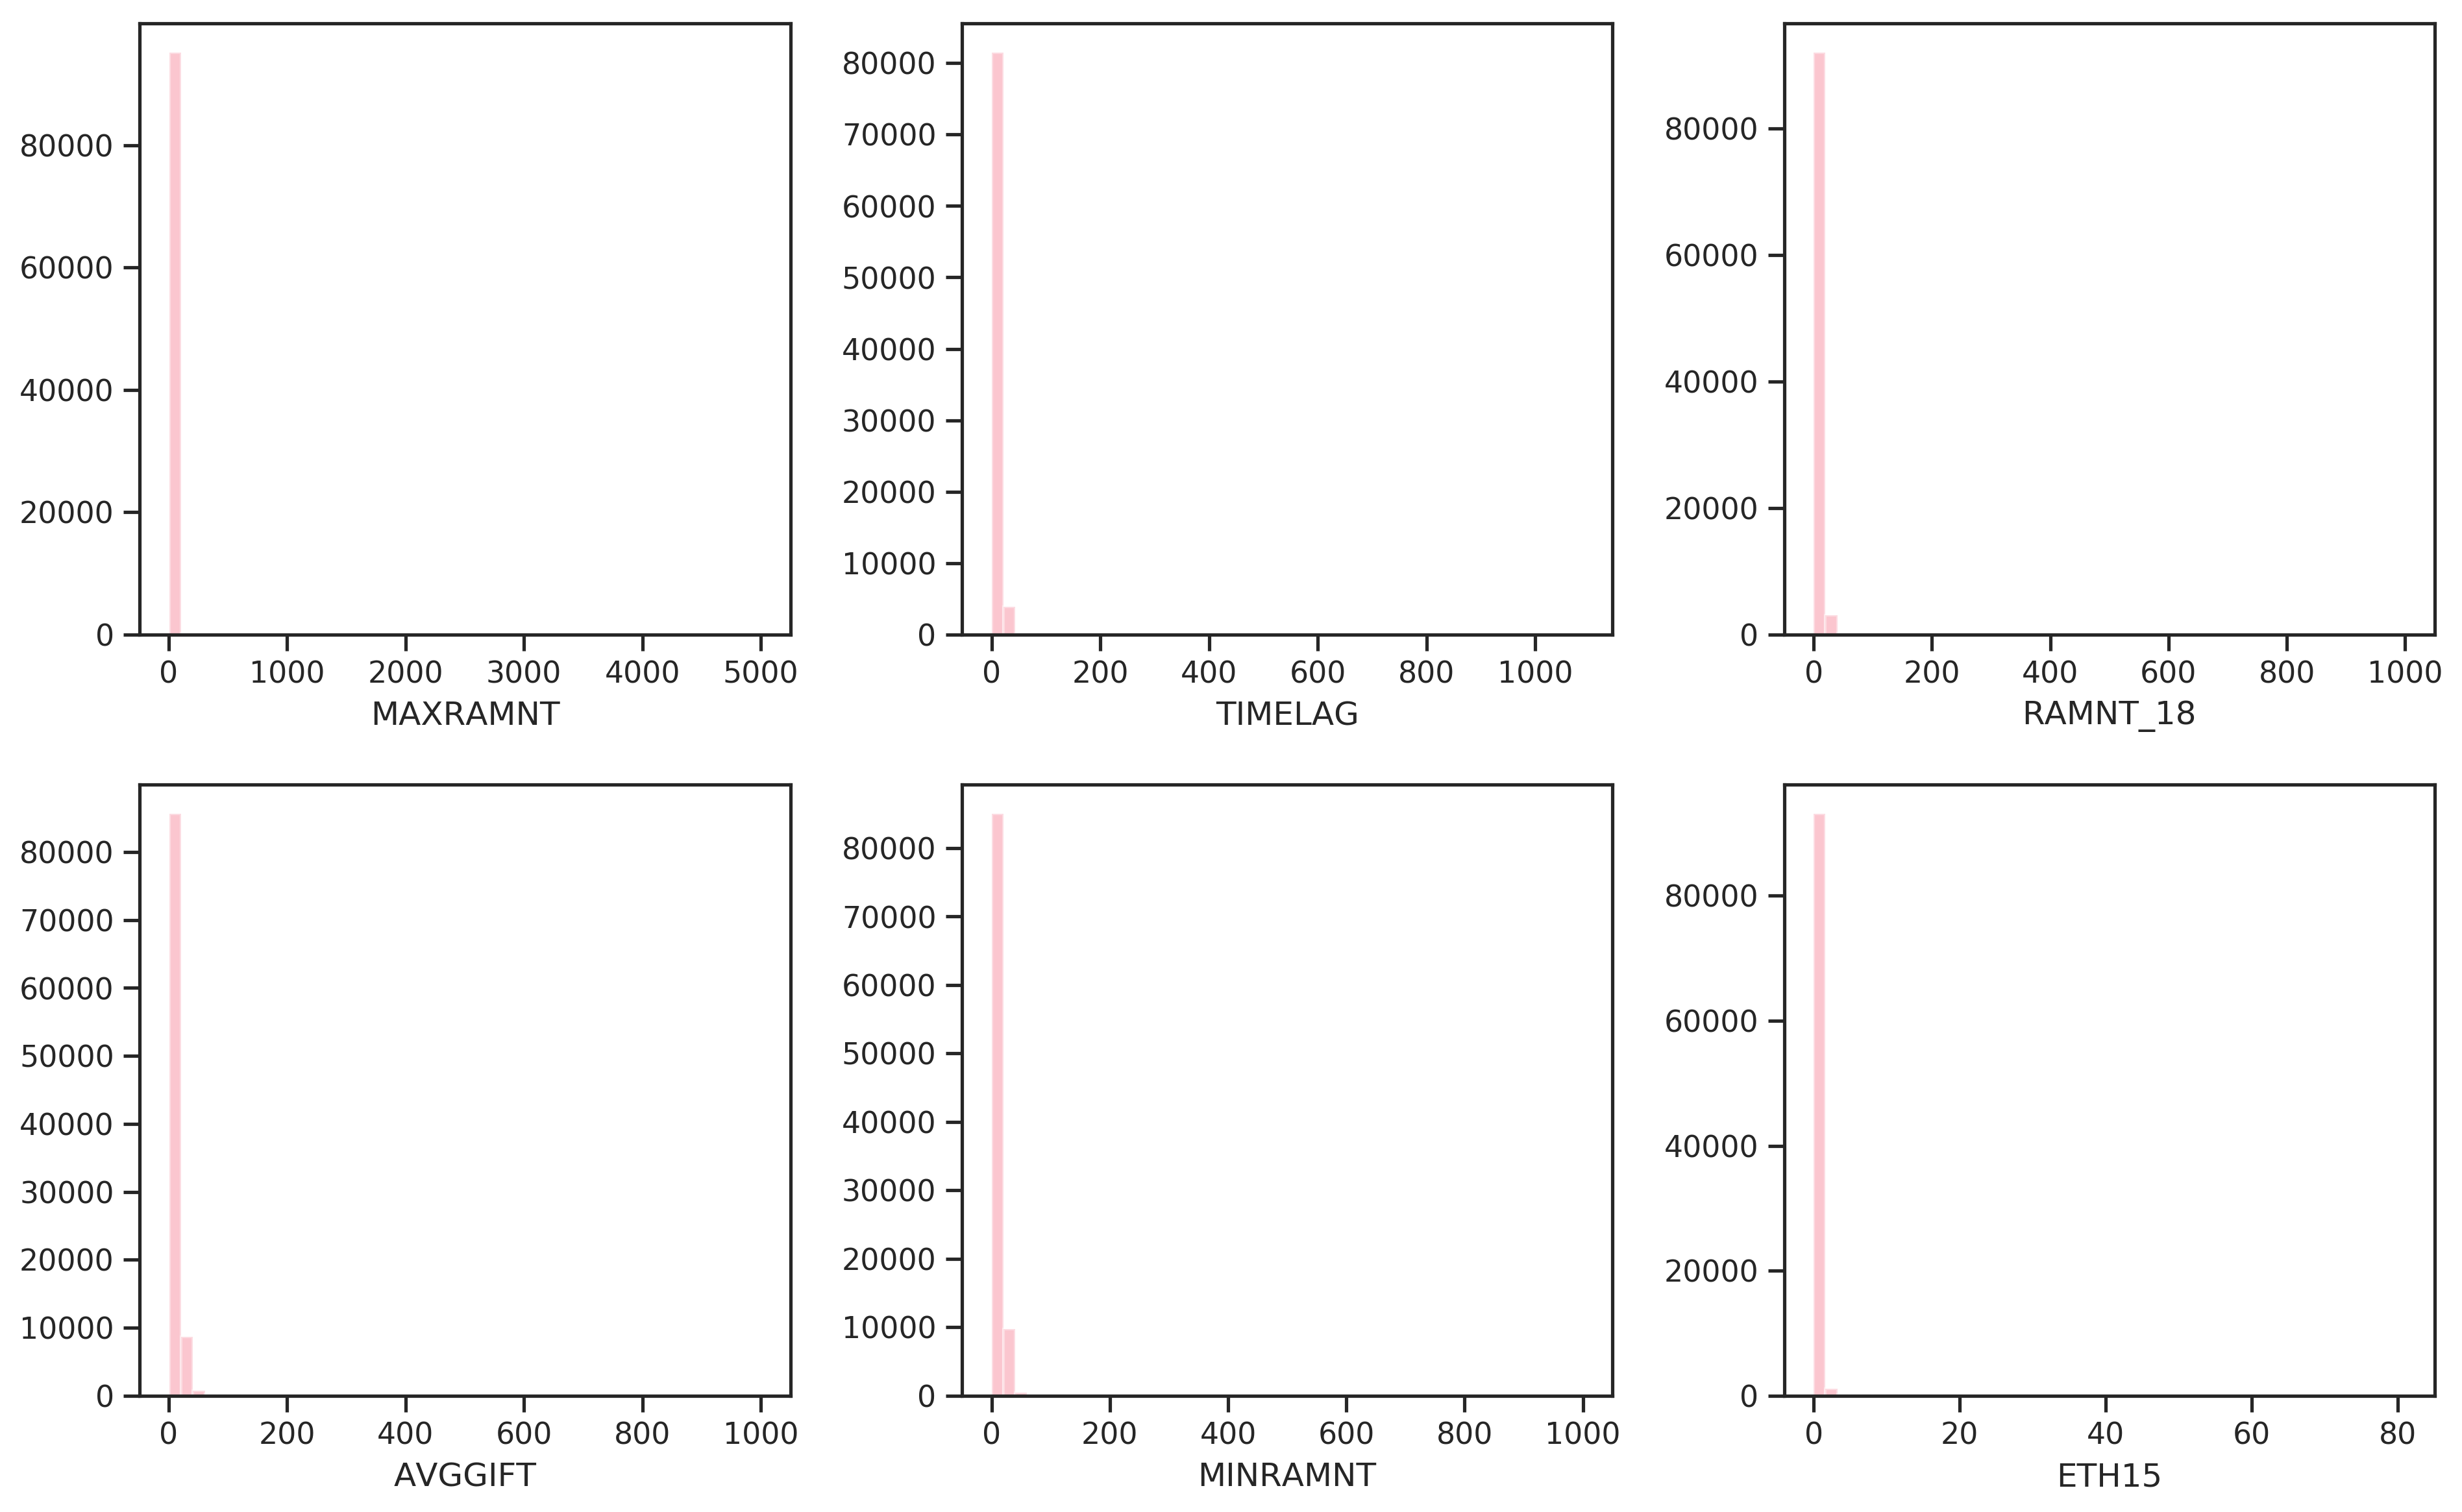
\includegraphics[width=0.7\linewidth]{figures/eda/most-skewed} 

}

\caption{The 9 most skewed features. Skewness metric: adjusted Fisher-Pearson standardized moment coefficient.}\label{fig:most-skewed}
\end{figure}

\hypertarget{targets}{%
\subsection{Targets}\label{targets}}

Of the two targets, one is binary (TARGET\_B), the other discrete (TARGET\_D). The former indicates whether an example has donated in response to the current promotion. The latter represents the dollar amount donated in response to the current promotion.

The distribution of \emph{TARGET\_D}, excluding non-donors, is shown in Figure \ref{fig:target-distrib}. Evidently, most donations are small. The range of donations is between 1 and 200 \$ with the 50-percentile at 13 \$. The most frequent donation amount is 10 \$. There are a few outliers for donations above 100 \$.

\begin{figure}

{\centering 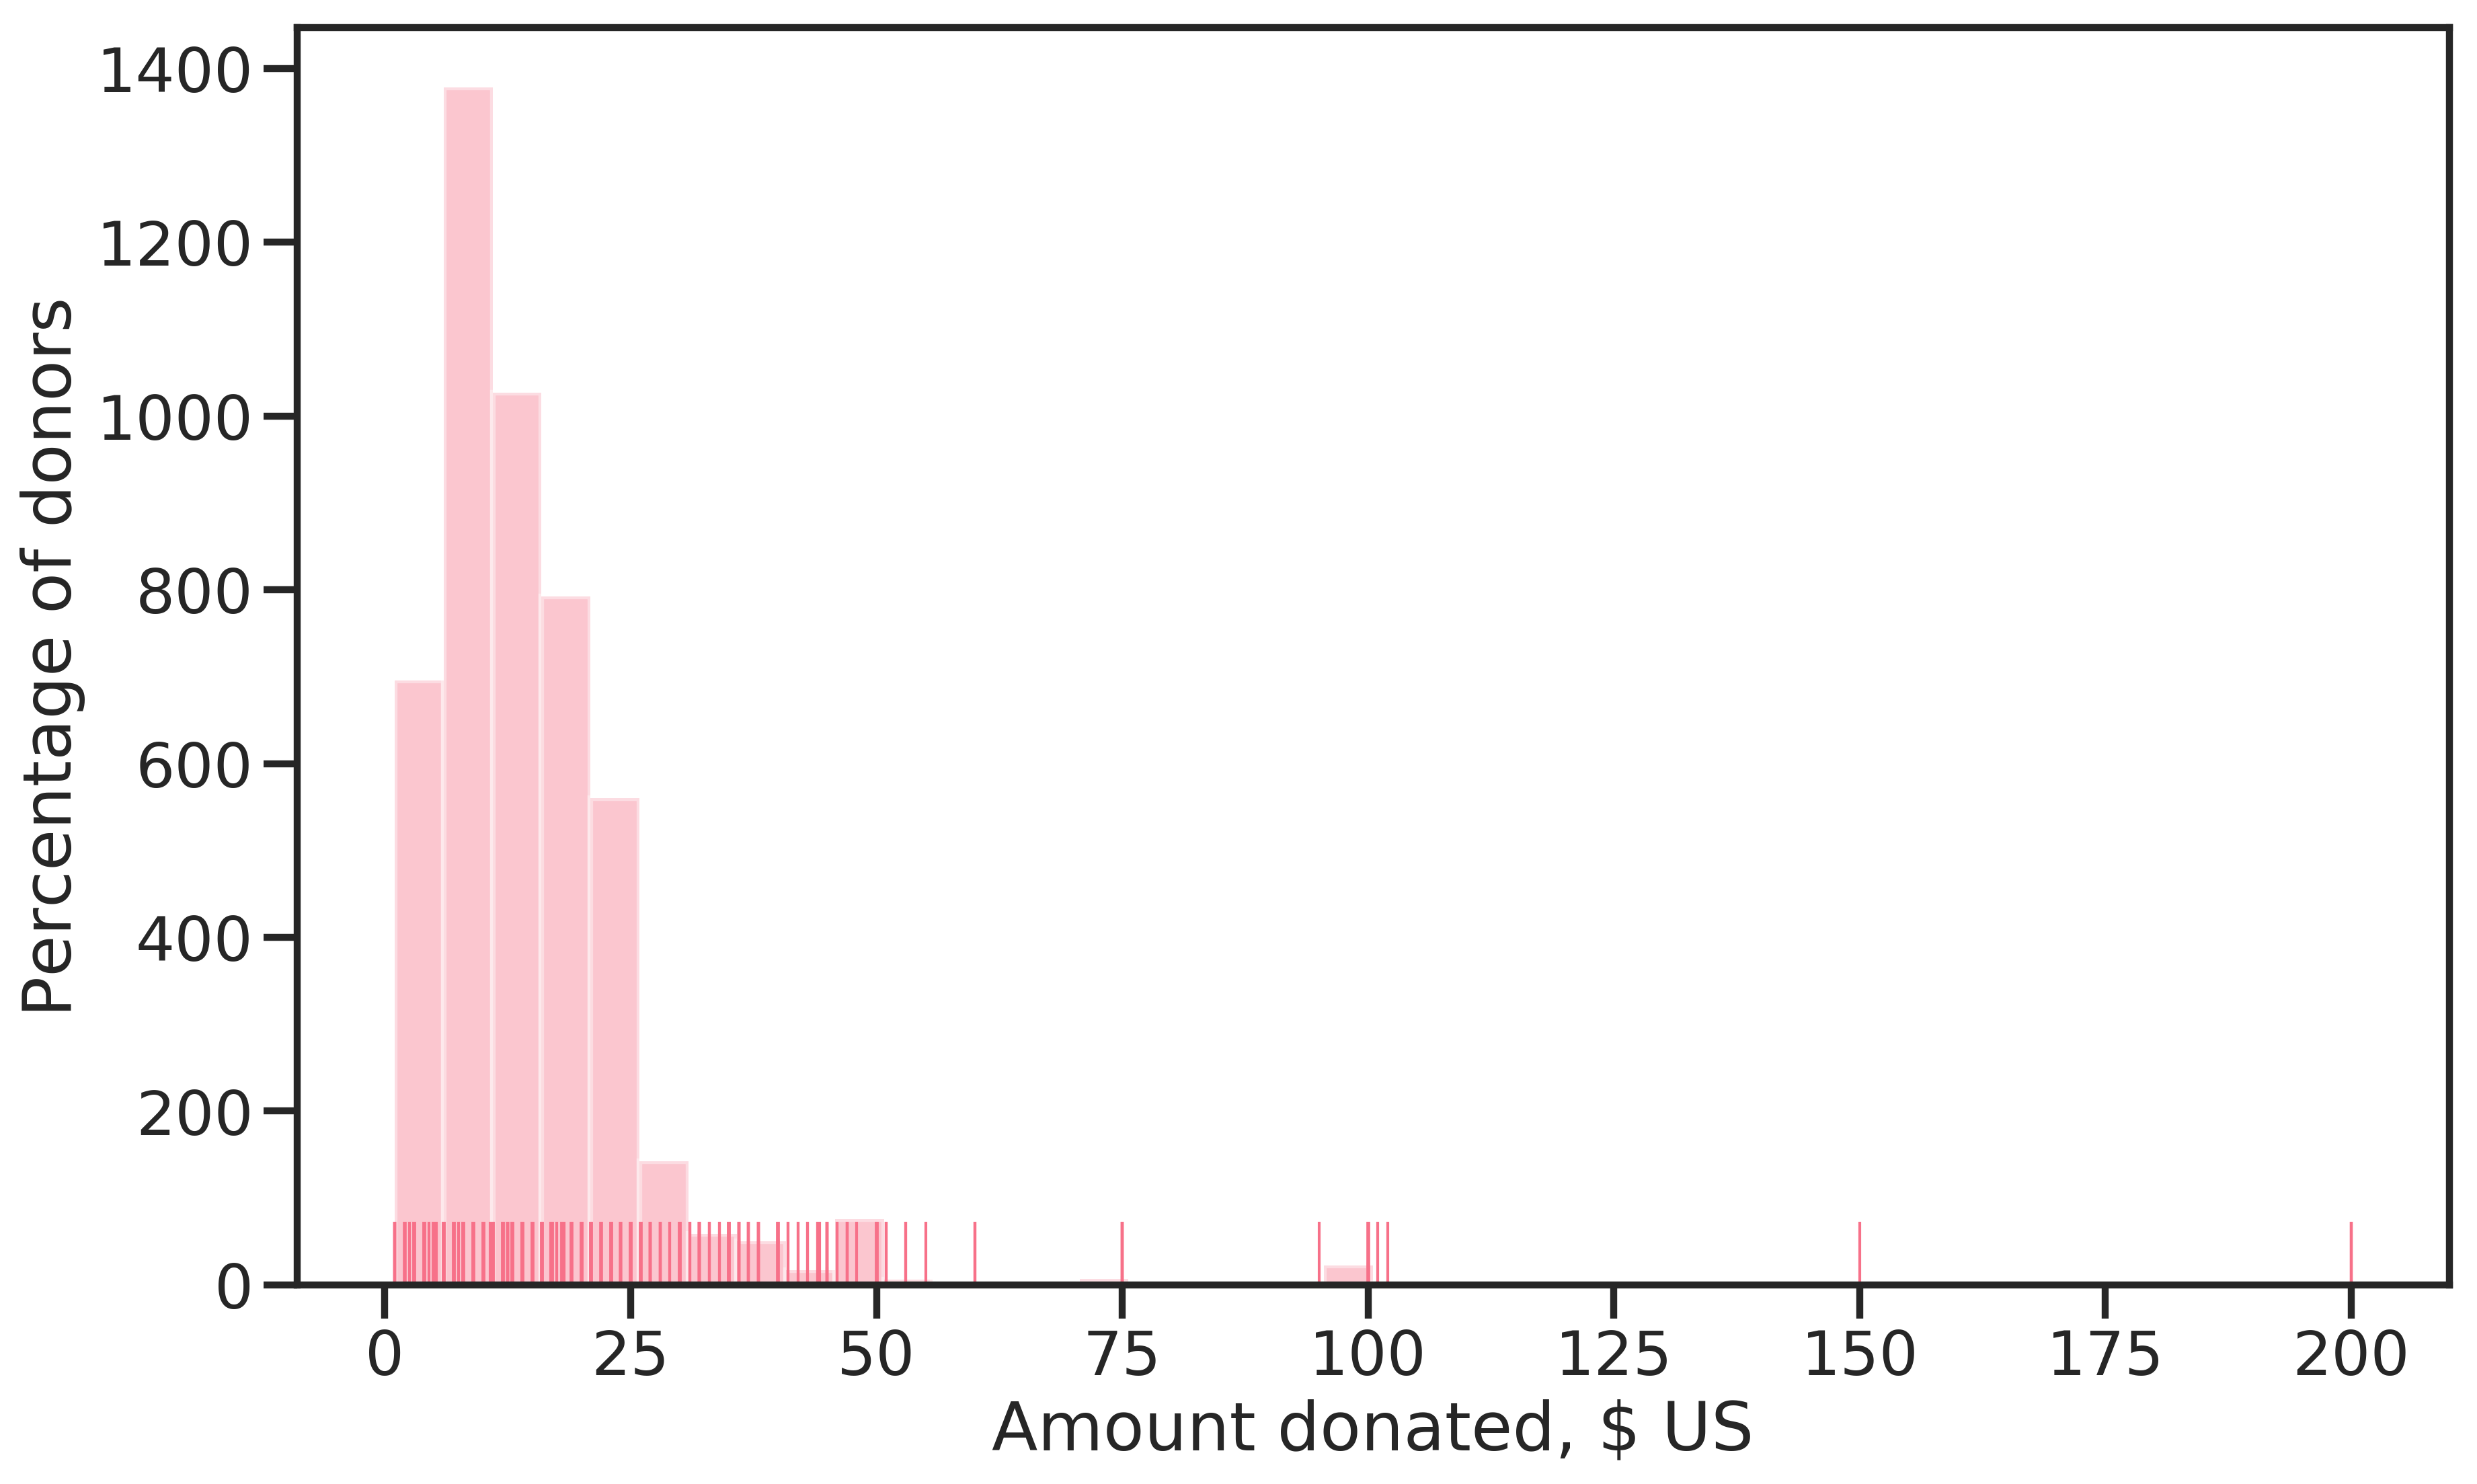
\includegraphics[width=0.7\linewidth]{figures/eda/target-distribution} 

}

\caption{Distribution of TARGETD. The donation amount in US dollar has a discrete distribution. Most donations are below 20 dollar, peaks are visible at 50, 75 and 100 dollar, while the maximum donation amount is 200 dollar.}\label{fig:target-distrib}
\end{figure}

As can be seen in Figure \ref{fig:target-ratio}, the target is imbalanced. Only about 5 \% of examples have donated. This poses a challenge in model training because there is a high risk of overfitting.

\begin{figure}

{\centering 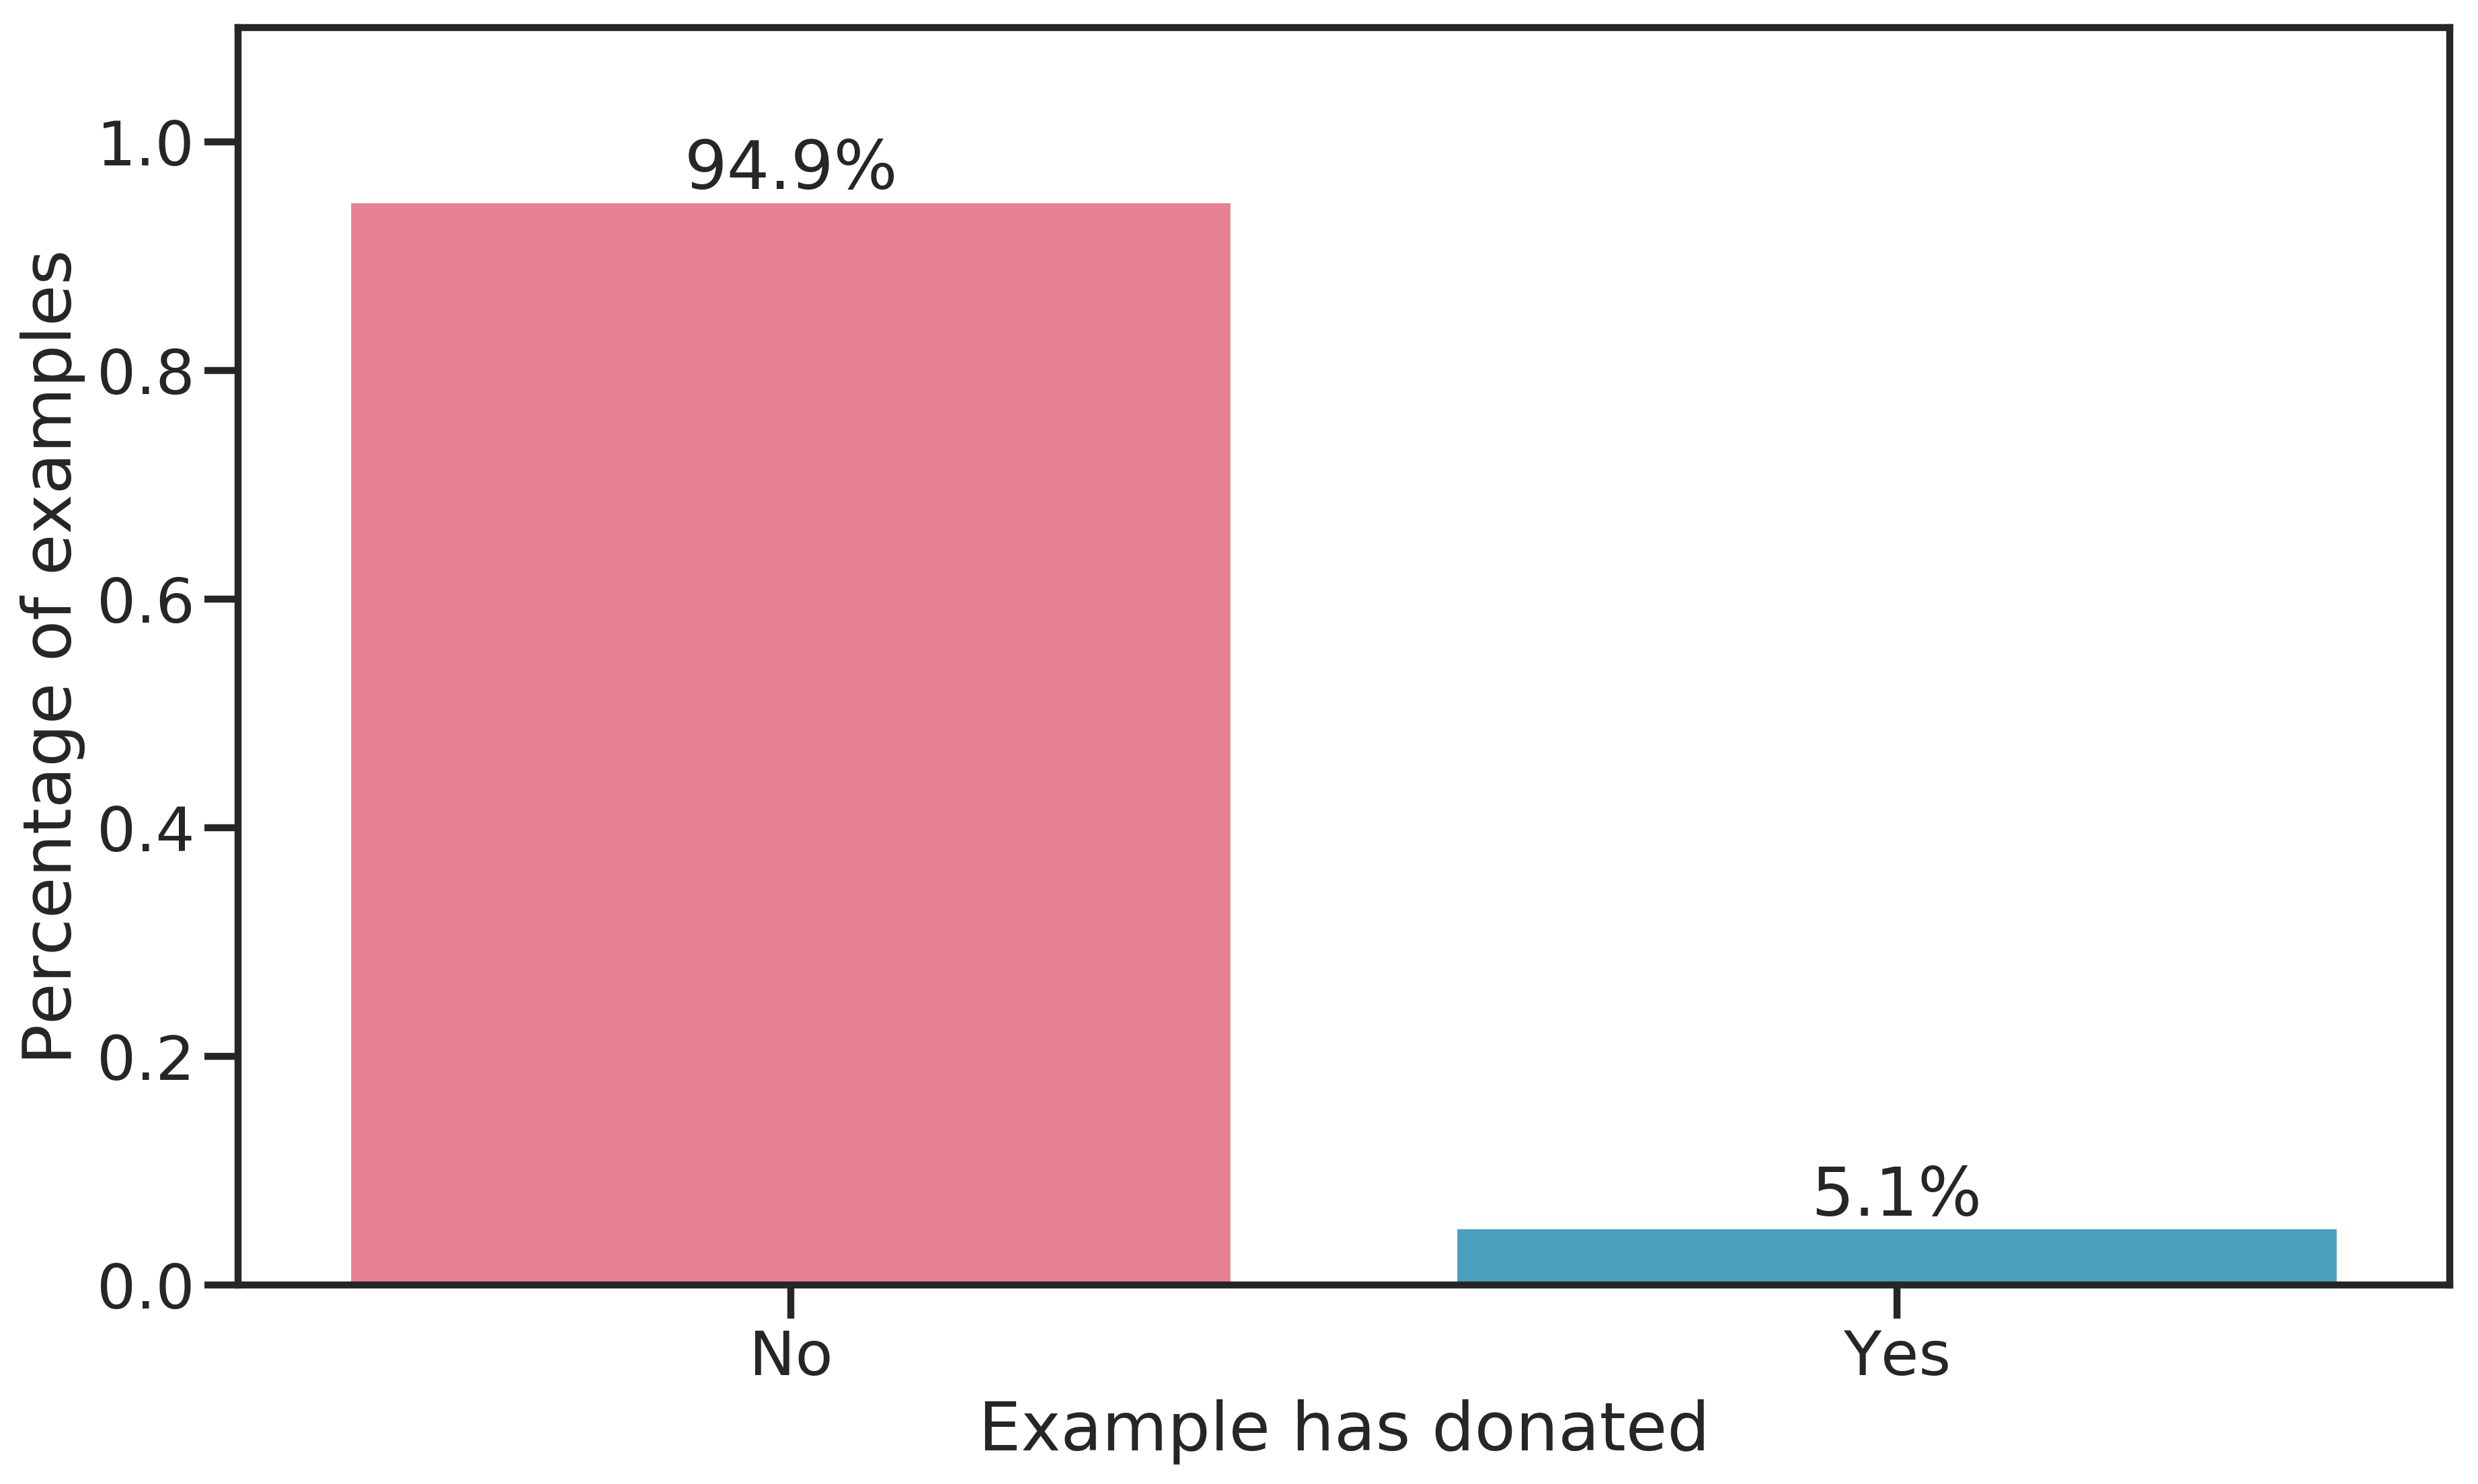
\includegraphics[width=0.7\linewidth]{figures/eda/ratio-binary} 

}

\caption{Ratio of donating examples. Less than 6 percent have made a donation.}\label{fig:target-ratio}
\end{figure}

\textbf{Datatypes}
An analysis of the dataset dictionary (see \ref{dataset-dictionary}) reveals the following datatypes for features:

\begin{itemize}
\tightlist
\item
  Index: CONTROLN, unique record identifier
\item
  Dates: 48 features in yymm format.
\item
  Binary: 30 features
\item
  Categorical: 90 features
\item
  Numeric: 286
\end{itemize}

\hypertarget{preprocessing}{%
\section{Preprocessing}\label{preprocessing}}

The dataset contains input errors (noisyness), features with datatypes that are impractical to work with (dates, categorical features) and redundant information. Furhtermore, many features contain missing values.

Noisy and categorical features were processed by the author manually before furhter evaluation of the data.
Handling of missing values, zero variance and sparse features was carried out through scikit-learn preprocessors.

\hypertarget{noisy-data}{%
\subsection{Noisy data}\label{noisy-data}}

There were two types of noisyness that were treated manually:

\begin{itemize}
\item
  Binary features with a mixture of 0, 1 and other codes
  Binary features were all recoded to \(\{\text{True},\text{False}\}\), preserving missing values. \(1\) was always set to \(\text{True}\) and \(0\) was coded \(\text{False}\). Specific mappings for \(\text{True} / \text{False}\) values given in the data dictionary per binary field were respected accordingly. As per the data dictionary, \(\text{' '}\) was interpreted as \(\text{False}\) for some features. For all other features, \(\text{' '}\) was interpreted as missing.
\item
  Dates are expected in \emph{mmyy} as per the dataset dictionary. For several date features, one digit was missing {[}EXPLAIN HOW FIXED{]}.
\item
  Zip codes: Input errors, inconsistent data (alphanumeric values)
\end{itemize}

\hypertarget{constant-features}{%
\subsection{Constant features}\label{constant-features}}

\begin{itemize}
\tightlist
\item
  Per the cup's documentation, features with zero variance have to be excluded.
\end{itemize}

\hypertarget{missing-values-sparse-features}{%
\subsection{Missing values / sparse features}\label{missing-values-sparse-features}}

\begin{itemize}
\tightlist
\item
  Character features: ' `,''
\item
  Numeric features: ' `,'`,'.'
\item
  Missing values are to be kept in the dataset for learning. Approriate methods for imputation are to be employed (median, mean, mode, modeled, \ldots{})
\item
  Exception: Features with more than 99.5 \% missing values are to be dropped
\item
  Features with a sparse distribution are to be dropped {[}DEFINITION???{]}
\end{itemize}

\hypertarget{categorical-features}{%
\subsection{Categorical features}\label{categorical-features}}

Several variables are aggregated into byte-wise codes (referred to as \emph{symbolic} fields in the data dictionary) that need to be spread out across separate variables.

Most machine-learning methods require strictly numerical data {[}REFERENCE{]}. Several methods exist to transform categorical (string-) values into a usable format. These include:

\begin{itemize}
\tightlist
\item
  One-hot tranformation: Creating dummy variables for each category level.
  This approach greatly increases dimensionality, which is both more resource-intensive and prone to overfitting.
\item
  Ordinal encoding: The categorical targets are transformed to ordinal values (integer numbers). This preserves dimensionality, but the algorithm chosen to assign the ordinal levels can introduce unwanted effects (an implied similarity based on closeness of the ordinal variables)
  Feature hashing: The individual values are hashed into a value of fixed length.
\item
  Hashing: {[}DEFINITION{]}
\end{itemize}

\hypertarget{feature-engineering-1}{%
\subsection{Feature Engineering}\label{feature-engineering-1}}

\hypertarget{feature-selection-1}{%
\subsection{Feature Selection}\label{feature-selection-1}}

-\textgreater{} Selecting the most useful features

\hypertarget{feature-extraction}{%
\subsection{Feature Extraction}\label{feature-extraction}}

-\textgreater{} Trying to group correlated features into one (dimensionality reduction). Unsupervised learning.

\hypertarget{model-evaluation-1}{%
\chapter{Model evaluation}\label{model-evaluation-1}}

Workflow:

Split training dataset 80/20 into training* and test

\begin{enumerate}
\def\labelenumi{\arabic{enumi}.}
\tightlist
\item
  Train on training* dataset
\item
  Adjust hyperparameters on validation set
\item
  Run on test dataset to get generalisation error estimate
\end{enumerate}

\hypertarget{results-and-discussion}{%
\chapter{Results and Discussion}\label{results-and-discussion}}

\hypertarget{conclusions}{%
\chapter{Conclusions}\label{conclusions}}

\hypertarget{comparison-with-cup-winners}{%
\section{Comparison with Cup winners}\label{comparison-with-cup-winners}}

The KDD-CUP committee evaluated the results based on the net revenue generated on the validation sample.
The measure used was the sum (the actual donation amount - \$0.68) over all records for which the expected revenue (or predicted value of the donation) is over \$0.68.
This measure is simple, objective and a direct measure of profit. Table 2 depicts the results. The participants are listed based on the last column.

\begin{table}[!h]

\caption{\label{tab:benchmark-cup-winners}Top five of the KDD-CUP participants. N* denotes the number for which the predicted donation amount is > $0.68. Sum is the total profit, meaning the donation minus $0.68 for each example.}
\centering
\resizebox{\linewidth}{!}{
\begin{tabular}{lrrrrrr}
\toprule
\multicolumn{1}{c}{ } & \multicolumn{1}{c}{ } & \multicolumn{5}{c}{Amount, \$} \\
\cmidrule(l{3pt}r{3pt}){3-7}
  & N* & Min & Mean & Std & Max & Sum\\
\midrule
GainSmarts & 56330 & -0.68 & 0.26 & 5.57 & 499.32 & 14712\\
SAS & 55838 & -0.68 & 0.26 & 5.64 & 499.32 & 14662\\
Quadstone & 57836 & -0.68 & 0.24 & 5.66 & 499.32 & 13954\\
CARRL & 55650 & -0.68 & 0.25 & 5.61 & 499.32 & 13825\\
Amdocs & 51906 & -0.68 & 0.27 & 5.69 & 499.32 & 13794\\
\bottomrule
\end{tabular}}
\end{table}

\hypertarget{references}{%
\chapter*{References}\label{references}}
\addcontentsline{toc}{chapter}{References}

\hypertarget{refs}{}
\leavevmode\hypertarget{ref-allaire2016rmarkdown}{}%
Allaire, J, Joe Cheng, Yihui Xie, Jonathan McPherson, Winston Chang, Jeff Allen, Hadley Wickham, Aron Atkins, Rob Hyndman, and Ruben Arslan. 2016. \emph{Rmarkdown: Dynamic Documents for R}. \emph{R Package Version}. Vol. 1.

\leavevmode\hypertarget{ref-bellman1957dynamic}{}%
Bellman, R., Rand Corporation, and Karreman Mathematics Research Collection. 1957. \emph{Dynamic Programming}. Rand Corporation Research Study. Princeton University Press. \url{https://books.google.de/books?id=wdtoPwAACAAJ}.

\leavevmode\hypertarget{ref-chen2016xgboost}{}%
Chen, Tianqi, and Carlos Guestrin. 2016. ``Xgboost: A Scalable Tree Boosting System.'' In \emph{Proceedings of the 22nd Acm Sigkdd International Conference on Knowledge Discovery and Data Mining}, 785--94. ACM.

\leavevmode\hypertarget{ref-freund1997decision}{}%
Freund, Yoav, and Robert E Schapire. 1997. ``A Decision-Theoretic Generalization of on-Line Learning and an Application to Boosting.'' \emph{Journal of Computer and System Sciences} 55 (1): 119--39.

\leavevmode\hypertarget{ref-Goodfellow-et-al-2016}{}%
Goodfellow, Ian, Yoshua Bengio, and Aaron Courville. 2016. \emph{Deep Learning}. MIT Press.

\leavevmode\hypertarget{ref-Kluyver:2016aa}{}%
Kluyver, Thomas, Benjamin Ragan-Kelley, Fernando Pérez, Brian Granger, Matthias Bussonnier, Jonathan Frederic, Kyle Kelley, et al. 2016. ``Jupyter Notebooks -- a Publishing Format for Reproducible Computational Workflows.'' Edited by F. Loizides and B. Schmidt. IOS Press.

\leavevmode\hypertarget{ref-knuth1984literate}{}%
Knuth, Donald Ervin. 1984. ``Literate Programming.'' \emph{The Computer Journal} 27 (2): 97--111.

\leavevmode\hypertarget{ref-kursa2010boruta}{}%
Kursa, Miron B, Witold R Rudnicki, and others. 2010. ``Feature Selection with the Boruta Package.'' \emph{J Stat Softw} 36 (11): 1--13.

\leavevmode\hypertarget{ref-mckinney-proc-scipy-2010}{}%
McKinney, Wes. 2010. ``Data Structures for Statistical Computing in Python.'' In \emph{Proceedings of the 9th Python in Science Conference}, edited by Stéfan van der Walt and Jarrod Millman, 51--56.

\leavevmode\hypertarget{ref-scikit-learn}{}%
Pedregosa, F., G. Varoquaux, A. Gramfort, V. Michel, B. Thirion, O. Grisel, M. Blondel, et al. 2011. ``Scikit-Learn: Machine Learning in Python.'' \emph{Journal of Machine Learning Research} 12: 2825--30.

\leavevmode\hypertarget{ref-CS-R9526}{}%
Rossum, G. van. 1995. ``Python Tutorial.'' CS-R9526. Amsterdam: Centrum voor Wiskunde en Informatica (CWI).

\leavevmode\hypertarget{ref-rubin1976inference}{}%
Rubin, Donald B. 1976. ``Inference and Missing Data.'' \emph{Biometrika} 63 (3): 581--92.

\leavevmode\hypertarget{ref-troyanskaya2001missing}{}%
Troyanskaya, Olga, Michael Cantor, Gavin Sherlock, Pat Brown, Trevor Hastie, Robert Tibshirani, David Botstein, and Russ B Altman. 2001. ``Missing Value Estimation Methods for Dna Microarrays.'' \emph{Bioinformatics} 17 (6): 520--25.

\leavevmode\hypertarget{ref-census-gazet}{}%
United States Census Bureau. 2018. ``2018 U.s. Gazetteer Files.'' 2018. \url{https://www.census.gov/geographies/reference-files/2018/geo/gazetter-file.html}.

\leavevmode\hypertarget{ref-xie2015}{}%
Xie, Yihui. 2015. \emph{Dynamic Documents with R and Knitr}. 2nd ed. Boca Raton, Florida: Chapman; Hall/CRC.

\leavevmode\hypertarget{ref-xie2016bookdown}{}%
---------. 2016. \emph{Bookdown: Authoring Books and Technical Documents with R Markdown}. Boca Raton, Florida: Chapman; Hall/CRC.

\hypertarget{appendix}{%
\chapter*{Appendix}\label{appendix}}
\addcontentsline{toc}{chapter}{Appendix}

\hypertarget{code}{%
\section{Code}\label{code}}

All code is also available online at \href{https://github.com/datarian/master-thesis-code}{github.com/datarian/master-thesis-code}

\hypertarget{preprocessing-1}{%
\subsection{Preprocessing}\label{preprocessing-1}}

\hypertarget{code-dateparser}{%
\subsubsection{Date parser}\label{code-dateparser}}

\begin{lstlisting}[language=Python,stepnumber=2,basicstyle=\footnotesize]
def dateparser(date_features):\end{lstlisting}
\begin{lstlisting}[language=Python,stepnumber=2,basicstyle=\footnotesize]
\end{lstlisting}
\begin{lstlisting}[language=Python,stepnumber=2,basicstyle=\footnotesize]
    def fix_format(d):\end{lstlisting}
\begin{lstlisting}[language=Python,stepnumber=2,basicstyle=\footnotesize]
        if not pd.isna(d):\end{lstlisting}
\begin{lstlisting}[language=Python,stepnumber=2,basicstyle=\footnotesize]
            if len(d) == 3:\end{lstlisting}
\begin{lstlisting}[language=Python,stepnumber=2,basicstyle=\footnotesize]
                d = '0'+d\end{lstlisting}
\begin{lstlisting}[language=Python,stepnumber=2,basicstyle=\footnotesize]
        else:\end{lstlisting}
\begin{lstlisting}[language=Python,stepnumber=2,basicstyle=\footnotesize]
            d = pd.NaT\end{lstlisting}
\begin{lstlisting}[language=Python,stepnumber=2,basicstyle=\footnotesize]
        return d\end{lstlisting}
\begin{lstlisting}[language=Python,stepnumber=2,basicstyle=\footnotesize]
\end{lstlisting}
\begin{lstlisting}[language=Python,stepnumber=2,basicstyle=\footnotesize]
    def fix_century(d):\end{lstlisting}
\begin{lstlisting}[language=Python,stepnumber=2,basicstyle=\footnotesize]
        ref_date = App.config("reference_date")\end{lstlisting}
\begin{lstlisting}[language=Python,stepnumber=2,basicstyle=\footnotesize]
        if not pd.isna(d):\end{lstlisting}
\begin{lstlisting}[language=Python,stepnumber=2,basicstyle=\footnotesize]
            try:\end{lstlisting}
\begin{lstlisting}[language=Python,stepnumber=2,basicstyle=\footnotesize]
                if d.year > ref_date.year:\end{lstlisting}
\begin{lstlisting}[language=Python,stepnumber=2,basicstyle=\footnotesize]
                    d = d.replace(year=(d.year-100))\end{lstlisting}
\begin{lstlisting}[language=Python,stepnumber=2,basicstyle=\footnotesize]
            except Exception as err:\end{lstlisting}
\begin{lstlisting}[language=Python,stepnumber=2,basicstyle=\footnotesize]
                logger.warning("Failed to fix century for date {}, reason: {}".format(d, err))\end{lstlisting}
\begin{lstlisting}[language=Python,stepnumber=2,basicstyle=\footnotesize]
                d = pd.NaT\end{lstlisting}
\begin{lstlisting}[language=Python,stepnumber=2,basicstyle=\footnotesize]
        else:\end{lstlisting}
\begin{lstlisting}[language=Python,stepnumber=2,basicstyle=\footnotesize]
            d = pd.NaT\end{lstlisting}
\begin{lstlisting}[language=Python,stepnumber=2,basicstyle=\footnotesize]
        return d\end{lstlisting}
\begin{lstlisting}[language=Python,stepnumber=2,basicstyle=\footnotesize]
\end{lstlisting}
\begin{lstlisting}[language=Python,stepnumber=2,basicstyle=\footnotesize]
    try:\end{lstlisting}
\begin{lstlisting}[language=Python,stepnumber=2,basicstyle=\footnotesize]
        date_features = [fix_century(pd.to_datetime(fix_format(d),\end{lstlisting}
\begin{lstlisting}[language=Python,stepnumber=2,basicstyle=\footnotesize]
                                     format="%y%m", errors="coerce"))\end{lstlisting}
\begin{lstlisting}[language=Python,stepnumber=2,basicstyle=\footnotesize]
                         for d in date_features]\end{lstlisting}
\begin{lstlisting}[language=Python,stepnumber=2,basicstyle=\footnotesize]
    except Exception as e:\end{lstlisting}
\begin{lstlisting}[language=Python,stepnumber=2,basicstyle=\footnotesize]
        logger.warn("Failed to parse date array {}.\nReason: {}".format(date_features, e))\end{lstlisting}
\begin{lstlisting}[language=Python,stepnumber=2,basicstyle=\footnotesize]
    return date_features\end{lstlisting}

\hypertarget{appendix-transformers}{%
\subsection{Transformers}\label{appendix-transformers}}

\begin{lstlisting}[language=Python,stepnumber=2,basicstyle=\footnotesize]
# -*- coding: utf-8 -*-\end{lstlisting}
\begin{lstlisting}[language=Python,stepnumber=2,basicstyle=\footnotesize]
"""\end{lstlisting}
\begin{lstlisting}[language=Python,stepnumber=2,basicstyle=\footnotesize]
Created on Fri Aug 24 10:18:44 2018\end{lstlisting}
\begin{lstlisting}[language=Python,stepnumber=2,basicstyle=\footnotesize]
@author: Florian Hochstrasser\end{lstlisting}
\begin{lstlisting}[language=Python,stepnumber=2,basicstyle=\footnotesize]
"""\end{lstlisting}
\begin{lstlisting}[language=Python,stepnumber=2,basicstyle=\footnotesize]
\end{lstlisting}
\begin{lstlisting}[language=Python,stepnumber=2,basicstyle=\footnotesize]
import copy\end{lstlisting}
\begin{lstlisting}[language=Python,stepnumber=2,basicstyle=\footnotesize]
import datetime\end{lstlisting}
\begin{lstlisting}[language=Python,stepnumber=2,basicstyle=\footnotesize]
import hashlib\end{lstlisting}
\begin{lstlisting}[language=Python,stepnumber=2,basicstyle=\footnotesize]
import logging\end{lstlisting}
\begin{lstlisting}[language=Python,stepnumber=2,basicstyle=\footnotesize]
import sys\end{lstlisting}
\begin{lstlisting}[language=Python,stepnumber=2,basicstyle=\footnotesize]
\end{lstlisting}
\begin{lstlisting}[language=Python,stepnumber=2,basicstyle=\footnotesize]
import numpy as np\end{lstlisting}
\begin{lstlisting}[language=Python,stepnumber=2,basicstyle=\footnotesize]
import pandas as pd\end{lstlisting}
\begin{lstlisting}[language=Python,stepnumber=2,basicstyle=\footnotesize]
from dateutil import relativedelta\end{lstlisting}
\begin{lstlisting}[language=Python,stepnumber=2,basicstyle=\footnotesize]
from dateutil.rrule import MONTHLY, YEARLY, rrule\end{lstlisting}
\begin{lstlisting}[language=Python,stepnumber=2,basicstyle=\footnotesize]
from sklearn.base import BaseEstimator, TransformerMixin\end{lstlisting}
\begin{lstlisting}[language=Python,stepnumber=2,basicstyle=\footnotesize]
\end{lstlisting}
\begin{lstlisting}[language=Python,stepnumber=2,basicstyle=\footnotesize]
from category_encoders import OrdinalEncoder\end{lstlisting}
\begin{lstlisting}[language=Python,stepnumber=2,basicstyle=\footnotesize]
\end{lstlisting}
\begin{lstlisting}[language=Python,stepnumber=2,basicstyle=\footnotesize]
# Set up the logger\end{lstlisting}
\begin{lstlisting}[language=Python,stepnumber=2,basicstyle=\footnotesize]
logging.basicConfig(filename=__name__+'.log', level=logging.ERROR)\end{lstlisting}
\begin{lstlisting}[language=Python,stepnumber=2,basicstyle=\footnotesize]
logger = logging.getLogger(__name__)\end{lstlisting}
\begin{lstlisting}[language=Python,stepnumber=2,basicstyle=\footnotesize]
\end{lstlisting}
\begin{lstlisting}[language=Python,stepnumber=2,basicstyle=\footnotesize]
\end{lstlisting}
\begin{lstlisting}[language=Python,stepnumber=2,basicstyle=\footnotesize]
__all__ = ['DropSparseLowVar',\end{lstlisting}
\begin{lstlisting}[language=Python,stepnumber=2,basicstyle=\footnotesize]
           'BinaryFeatureRecode',\end{lstlisting}
\begin{lstlisting}[language=Python,stepnumber=2,basicstyle=\footnotesize]
           'MultiByteExtract',\end{lstlisting}
\begin{lstlisting}[language=Python,stepnumber=2,basicstyle=\footnotesize]
           'RecodeUrbanSocioEconomic',\end{lstlisting}
\begin{lstlisting}[language=Python,stepnumber=2,basicstyle=\footnotesize]
           'DeltaTime',\end{lstlisting}
\begin{lstlisting}[language=Python,stepnumber=2,basicstyle=\footnotesize]
           'MonthsToDonation']\end{lstlisting}
\begin{lstlisting}[language=Python,stepnumber=2,basicstyle=\footnotesize]
\end{lstlisting}
\begin{lstlisting}[language=Python,stepnumber=2,basicstyle=\footnotesize]
\end{lstlisting}
\begin{lstlisting}[language=Python,stepnumber=2,basicstyle=\footnotesize]
class DropSparseLowVar(BaseEstimator, TransformerMixin):\end{lstlisting}
\begin{lstlisting}[language=Python,stepnumber=2,basicstyle=\footnotesize]
    """ Transformer to drop:\end{lstlisting}
\begin{lstlisting}[language=Python,stepnumber=2,basicstyle=\footnotesize]
\end{lstlisting}
\begin{lstlisting}[language=Python,stepnumber=2,basicstyle=\footnotesize]
    * low variance\end{lstlisting}
\begin{lstlisting}[language=Python,stepnumber=2,basicstyle=\footnotesize]
    * sparse (abundance of NaN)\end{lstlisting}
\begin{lstlisting}[language=Python,stepnumber=2,basicstyle=\footnotesize]
    features.\end{lstlisting}
\begin{lstlisting}[language=Python,stepnumber=2,basicstyle=\footnotesize]
\end{lstlisting}
\begin{lstlisting}[language=Python,stepnumber=2,basicstyle=\footnotesize]
    Parameters:\end{lstlisting}
\begin{lstlisting}[language=Python,stepnumber=2,basicstyle=\footnotesize]
    -----------\end{lstlisting}
\begin{lstlisting}[language=Python,stepnumber=2,basicstyle=\footnotesize]
\end{lstlisting}
\begin{lstlisting}[language=Python,stepnumber=2,basicstyle=\footnotesize]
    * var_threshold float\end{lstlisting}
\begin{lstlisting}[language=Python,stepnumber=2,basicstyle=\footnotesize]
        Defines the threshold for the variance below which columns\end{lstlisting}
\begin{lstlisting}[language=Python,stepnumber=2,basicstyle=\footnotesize]
        are interpreted as constant.\end{lstlisting}
\begin{lstlisting}[language=Python,stepnumber=2,basicstyle=\footnotesize]
    * sparse_threshold loat\end{lstlisting}
\begin{lstlisting}[language=Python,stepnumber=2,basicstyle=\footnotesize]
        Defines the threshold (percentage) of NaN's in a column, anything\end{lstlisting}
\begin{lstlisting}[language=Python,stepnumber=2,basicstyle=\footnotesize]
        having greater than this percentage NaN's will be discarded.\end{lstlisting}
\begin{lstlisting}[language=Python,stepnumber=2,basicstyle=\footnotesize]
    """\end{lstlisting}
\begin{lstlisting}[language=Python,stepnumber=2,basicstyle=\footnotesize]
\end{lstlisting}
\begin{lstlisting}[language=Python,stepnumber=2,basicstyle=\footnotesize]
    def __init__(self, var_threshold=1e-5, sparse_threshold=0.1,\end{lstlisting}
\begin{lstlisting}[language=Python,stepnumber=2,basicstyle=\footnotesize]
                 keep_anyways=[]):\end{lstlisting}
\begin{lstlisting}[language=Python,stepnumber=2,basicstyle=\footnotesize]
        """\end{lstlisting}
\begin{lstlisting}[language=Python,stepnumber=2,basicstyle=\footnotesize]
        Removes features with either a low variance or\end{lstlisting}
\begin{lstlisting}[language=Python,stepnumber=2,basicstyle=\footnotesize]
        those that contain only very few non-NAN's.\end{lstlisting}
\begin{lstlisting}[language=Python,stepnumber=2,basicstyle=\footnotesize]
\end{lstlisting}
\begin{lstlisting}[language=Python,stepnumber=2,basicstyle=\footnotesize]
        Parameters:\end{lstlisting}
\begin{lstlisting}[language=Python,stepnumber=2,basicstyle=\footnotesize]
        -----------\end{lstlisting}
\begin{lstlisting}[language=Python,stepnumber=2,basicstyle=\footnotesize]
\end{lstlisting}
\begin{lstlisting}[language=Python,stepnumber=2,basicstyle=\footnotesize]
        var_threshold: float. Anything lower than this\end{lstlisting}
\begin{lstlisting}[language=Python,stepnumber=2,basicstyle=\footnotesize]
                       is considered constant and dropped.\end{lstlisting}
\begin{lstlisting}[language=Python,stepnumber=2,basicstyle=\footnotesize]
        sparse_threshold: Minimum percentage of non-NaN's needed to keep\end{lstlisting}
\begin{lstlisting}[language=Python,stepnumber=2,basicstyle=\footnotesize]
                          a feature\end{lstlisting}
\begin{lstlisting}[language=Python,stepnumber=2,basicstyle=\footnotesize]
        keep_anyways: List of regex patterns for features to keep regardless of\end{lstlisting}
\begin{lstlisting}[language=Python,stepnumber=2,basicstyle=\footnotesize]
            variance / sparsity.\end{lstlisting}
\begin{lstlisting}[language=Python,stepnumber=2,basicstyle=\footnotesize]
        """\end{lstlisting}
\begin{lstlisting}[language=Python,stepnumber=2,basicstyle=\footnotesize]
        self.thresh_var = var_threshold\end{lstlisting}
\begin{lstlisting}[language=Python,stepnumber=2,basicstyle=\footnotesize]
        self.thresh_sparse = sparse_threshold\end{lstlisting}
\begin{lstlisting}[language=Python,stepnumber=2,basicstyle=\footnotesize]
        self.feature_names = []\end{lstlisting}
\begin{lstlisting}[language=Python,stepnumber=2,basicstyle=\footnotesize]
        self.drop_names = []\end{lstlisting}
\begin{lstlisting}[language=Python,stepnumber=2,basicstyle=\footnotesize]
        self. is_transformed = False\end{lstlisting}
\begin{lstlisting}[language=Python,stepnumber=2,basicstyle=\footnotesize]
        self.keep_anyways = keep_anyways\end{lstlisting}
\begin{lstlisting}[language=Python,stepnumber=2,basicstyle=\footnotesize]
\end{lstlisting}
\begin{lstlisting}[language=Python,stepnumber=2,basicstyle=\footnotesize]
    def fit(self, X, y=None):\end{lstlisting}
\begin{lstlisting}[language=Python,stepnumber=2,basicstyle=\footnotesize]
        assert isinstance(X, pd.DataFrame)\end{lstlisting}
\begin{lstlisting}[language=Python,stepnumber=2,basicstyle=\footnotesize]
        nrow = X.shape[0]\end{lstlisting}
\begin{lstlisting}[language=Python,stepnumber=2,basicstyle=\footnotesize]
\end{lstlisting}
\begin{lstlisting}[language=Python,stepnumber=2,basicstyle=\footnotesize]
        keep_names = set()\end{lstlisting}
\begin{lstlisting}[language=Python,stepnumber=2,basicstyle=\footnotesize]
        for search in self.keep_anyways:\end{lstlisting}
\begin{lstlisting}[language=Python,stepnumber=2,basicstyle=\footnotesize]
            print(X.filter(regex=search).columns)\end{lstlisting}
\begin{lstlisting}[language=Python,stepnumber=2,basicstyle=\footnotesize]
            keep_names.update(X.filter(regex=search).columns)\end{lstlisting}
\begin{lstlisting}[language=Python,stepnumber=2,basicstyle=\footnotesize]
\end{lstlisting}
\begin{lstlisting}[language=Python,stepnumber=2,basicstyle=\footnotesize]
        sparse_names = set(\end{lstlisting}
\begin{lstlisting}[language=Python,stepnumber=2,basicstyle=\footnotesize]
            [c for c in X if X[c].count() / nrow >= self.thresh_sparse]) - keep_names\end{lstlisting}
\begin{lstlisting}[language=Python,stepnumber=2,basicstyle=\footnotesize]
\end{lstlisting}
\begin{lstlisting}[language=Python,stepnumber=2,basicstyle=\footnotesize]
        low_var_names = set([c for c in X.select_dtypes(\end{lstlisting}
\begin{lstlisting}[language=Python,stepnumber=2,basicstyle=\footnotesize]
            include="number") if X[c].var() <= self.thresh_var]) - keep_names\end{lstlisting}
\begin{lstlisting}[language=Python,stepnumber=2,basicstyle=\footnotesize]
\end{lstlisting}
\begin{lstlisting}[language=Python,stepnumber=2,basicstyle=\footnotesize]
        self.drop_names = list(sparse_names.union(low_var_names))\end{lstlisting}
\begin{lstlisting}[language=Python,stepnumber=2,basicstyle=\footnotesize]
        print("Constant features: " + str(low_var_names))\end{lstlisting}
\begin{lstlisting}[language=Python,stepnumber=2,basicstyle=\footnotesize]
        print("Sparse features: " + str(sparse_names))\end{lstlisting}
\begin{lstlisting}[language=Python,stepnumber=2,basicstyle=\footnotesize]
        print("Keep anyways features: " + str(keep_names))\end{lstlisting}
\begin{lstlisting}[language=Python,stepnumber=2,basicstyle=\footnotesize]
        print(self.drop_names.sort())\end{lstlisting}
\begin{lstlisting}[language=Python,stepnumber=2,basicstyle=\footnotesize]
        return self\end{lstlisting}
\begin{lstlisting}[language=Python,stepnumber=2,basicstyle=\footnotesize]
\end{lstlisting}
\begin{lstlisting}[language=Python,stepnumber=2,basicstyle=\footnotesize]
    def transform(self, X, y=None):\end{lstlisting}
\begin{lstlisting}[language=Python,stepnumber=2,basicstyle=\footnotesize]
        X_trans = X.copy()\end{lstlisting}
\begin{lstlisting}[language=Python,stepnumber=2,basicstyle=\footnotesize]
        X_trans = X_trans.drop(columns=self.drop_names)\end{lstlisting}
\begin{lstlisting}[language=Python,stepnumber=2,basicstyle=\footnotesize]
        self.feature_names = X_trans.columns\end{lstlisting}
\begin{lstlisting}[language=Python,stepnumber=2,basicstyle=\footnotesize]
        self.is_transformed = True\end{lstlisting}
\begin{lstlisting}[language=Python,stepnumber=2,basicstyle=\footnotesize]
        return X_trans\end{lstlisting}
\begin{lstlisting}[language=Python,stepnumber=2,basicstyle=\footnotesize]
\end{lstlisting}
\begin{lstlisting}[language=Python,stepnumber=2,basicstyle=\footnotesize]
    def get_feature_names(self):\end{lstlisting}
\begin{lstlisting}[language=Python,stepnumber=2,basicstyle=\footnotesize]
        if not isinstance(self.is_transformed, list):\end{lstlisting}
\begin{lstlisting}[language=Python,stepnumber=2,basicstyle=\footnotesize]
            raise ValueError("Must be transformed first.")\end{lstlisting}
\begin{lstlisting}[language=Python,stepnumber=2,basicstyle=\footnotesize]
        return self.feature_names\end{lstlisting}
\begin{lstlisting}[language=Python,stepnumber=2,basicstyle=\footnotesize]
\end{lstlisting}
\begin{lstlisting}[language=Python,stepnumber=2,basicstyle=\footnotesize]
\end{lstlisting}
\begin{lstlisting}[language=Python,stepnumber=2,basicstyle=\footnotesize]
class MultiByteExtract(BaseEstimator, TransformerMixin):\end{lstlisting}
\begin{lstlisting}[language=Python,stepnumber=2,basicstyle=\footnotesize]
    """\end{lstlisting}
\begin{lstlisting}[language=Python,stepnumber=2,basicstyle=\footnotesize]
    This is a transformer for multibyte features. Each byte in such\end{lstlisting}
\begin{lstlisting}[language=Python,stepnumber=2,basicstyle=\footnotesize]
    a multibyte feature is actually a categorical feature.\end{lstlisting}
\begin{lstlisting}[language=Python,stepnumber=2,basicstyle=\footnotesize]
\end{lstlisting}
\begin{lstlisting}[language=Python,stepnumber=2,basicstyle=\footnotesize]
    The bytes are spread into separate categoricals.\end{lstlisting}
\begin{lstlisting}[language=Python,stepnumber=2,basicstyle=\footnotesize]
\end{lstlisting}
\begin{lstlisting}[language=Python,stepnumber=2,basicstyle=\footnotesize]
    Params:\end{lstlisting}
\begin{lstlisting}[language=Python,stepnumber=2,basicstyle=\footnotesize]
    -------\end{lstlisting}
\begin{lstlisting}[language=Python,stepnumber=2,basicstyle=\footnotesize]
    field_names: A list with the new names for each byte\end{lstlisting}
\begin{lstlisting}[language=Python,stepnumber=2,basicstyle=\footnotesize]
                    that is to be spread\end{lstlisting}
\begin{lstlisting}[language=Python,stepnumber=2,basicstyle=\footnotesize]
\end{lstlisting}
\begin{lstlisting}[language=Python,stepnumber=2,basicstyle=\footnotesize]
    impute: False means missing / malformatted entries will be coded NaN\end{lstlisting}
\begin{lstlisting}[language=Python,stepnumber=2,basicstyle=\footnotesize]
            If a value is passed, fields will be filled with that instead.\end{lstlisting}
\begin{lstlisting}[language=Python,stepnumber=2,basicstyle=\footnotesize]
\end{lstlisting}
\begin{lstlisting}[language=Python,stepnumber=2,basicstyle=\footnotesize]
    drop_orig: Whether to drop the original multibyte feature or not.\end{lstlisting}
\begin{lstlisting}[language=Python,stepnumber=2,basicstyle=\footnotesize]
    """\end{lstlisting}
\begin{lstlisting}[language=Python,stepnumber=2,basicstyle=\footnotesize]
\end{lstlisting}
\begin{lstlisting}[language=Python,stepnumber=2,basicstyle=\footnotesize]
    def __init__(self, field_names, impute=False, drop_orig=True):\end{lstlisting}
\begin{lstlisting}[language=Python,stepnumber=2,basicstyle=\footnotesize]
        self.field_names = field_names\end{lstlisting}
\begin{lstlisting}[language=Python,stepnumber=2,basicstyle=\footnotesize]
        # determines how many bytes to extract\end{lstlisting}
\begin{lstlisting}[language=Python,stepnumber=2,basicstyle=\footnotesize]
        self.sigbytes = len(self.field_names)\end{lstlisting}
\begin{lstlisting}[language=Python,stepnumber=2,basicstyle=\footnotesize]
        self.impute = impute\end{lstlisting}
\begin{lstlisting}[language=Python,stepnumber=2,basicstyle=\footnotesize]
        self.drop_orig = drop_orig\end{lstlisting}
\begin{lstlisting}[language=Python,stepnumber=2,basicstyle=\footnotesize]
        self.feature_names = []\end{lstlisting}
\begin{lstlisting}[language=Python,stepnumber=2,basicstyle=\footnotesize]
        self.is_transformed = False\end{lstlisting}
\begin{lstlisting}[language=Python,stepnumber=2,basicstyle=\footnotesize]
\end{lstlisting}
\begin{lstlisting}[language=Python,stepnumber=2,basicstyle=\footnotesize]
    def fit(self, X, y=None):\end{lstlisting}
\begin{lstlisting}[language=Python,stepnumber=2,basicstyle=\footnotesize]
        assert isinstance(X, pd.DataFrame)\end{lstlisting}
\begin{lstlisting}[language=Python,stepnumber=2,basicstyle=\footnotesize]
        self.feature_names = list(X.columns)\end{lstlisting}
\begin{lstlisting}[language=Python,stepnumber=2,basicstyle=\footnotesize]
        return self\end{lstlisting}
\begin{lstlisting}[language=Python,stepnumber=2,basicstyle=\footnotesize]
\end{lstlisting}
\begin{lstlisting}[language=Python,stepnumber=2,basicstyle=\footnotesize]
    def _fill_missing(self):\end{lstlisting}
\begin{lstlisting}[language=Python,stepnumber=2,basicstyle=\footnotesize]
        if not self.impute:\end{lstlisting}
\begin{lstlisting}[language=Python,stepnumber=2,basicstyle=\footnotesize]
            return [np.nan]*self.sigbytes\end{lstlisting}
\begin{lstlisting}[language=Python,stepnumber=2,basicstyle=\footnotesize]
        else:\end{lstlisting}
\begin{lstlisting}[language=Python,stepnumber=2,basicstyle=\footnotesize]
            return [self.impute]*self.sigbytes\end{lstlisting}
\begin{lstlisting}[language=Python,stepnumber=2,basicstyle=\footnotesize]
\end{lstlisting}
\begin{lstlisting}[language=Python,stepnumber=2,basicstyle=\footnotesize]
    def _spread(self, feature, index_name):\end{lstlisting}
\begin{lstlisting}[language=Python,stepnumber=2,basicstyle=\footnotesize]
        """ Fills the byte dataset for each record\end{lstlisting}
\begin{lstlisting}[language=Python,stepnumber=2,basicstyle=\footnotesize]
        Params:\end{lstlisting}
\begin{lstlisting}[language=Python,stepnumber=2,basicstyle=\footnotesize]
        -------\end{lstlisting}
\begin{lstlisting}[language=Python,stepnumber=2,basicstyle=\footnotesize]
        feature: A pandas series\end{lstlisting}
\begin{lstlisting}[language=Python,stepnumber=2,basicstyle=\footnotesize]
        """\end{lstlisting}
\begin{lstlisting}[language=Python,stepnumber=2,basicstyle=\footnotesize]
        # Dict to hold the split bytes\end{lstlisting}
\begin{lstlisting}[language=Python,stepnumber=2,basicstyle=\footnotesize]
        spread_field = {}\end{lstlisting}
\begin{lstlisting}[language=Python,stepnumber=2,basicstyle=\footnotesize]
        # Iterate over all rows, fill dict\end{lstlisting}
\begin{lstlisting}[language=Python,stepnumber=2,basicstyle=\footnotesize]
        for row in pd.DataFrame(feature).itertuples(name=None):\end{lstlisting}
\begin{lstlisting}[language=Python,stepnumber=2,basicstyle=\footnotesize]
            # row[0] is the index, row[1] the content of the cell\end{lstlisting}
\begin{lstlisting}[language=Python,stepnumber=2,basicstyle=\footnotesize]
            if not row[1] is np.nan:\end{lstlisting}
\begin{lstlisting}[language=Python,stepnumber=2,basicstyle=\footnotesize]
                if len(row[1]) == self.sigbytes:\end{lstlisting}
\begin{lstlisting}[language=Python,stepnumber=2,basicstyle=\footnotesize]
                    spread_field[row[0]] = list(row[1])\end{lstlisting}
\begin{lstlisting}[language=Python,stepnumber=2,basicstyle=\footnotesize]
                else:\end{lstlisting}
\begin{lstlisting}[language=Python,stepnumber=2,basicstyle=\footnotesize]
                    # The field is invalid\end{lstlisting}
\begin{lstlisting}[language=Python,stepnumber=2,basicstyle=\footnotesize]
                    spread_field[row[0]] = self._fill_missing()\end{lstlisting}
\begin{lstlisting}[language=Python,stepnumber=2,basicstyle=\footnotesize]
            else:\end{lstlisting}
\begin{lstlisting}[language=Python,stepnumber=2,basicstyle=\footnotesize]
                # handle missing values\end{lstlisting}
\begin{lstlisting}[language=Python,stepnumber=2,basicstyle=\footnotesize]
                spread_field[row[0]] = self._fill_missing()\end{lstlisting}
\begin{lstlisting}[language=Python,stepnumber=2,basicstyle=\footnotesize]
\end{lstlisting}
\begin{lstlisting}[language=Python,stepnumber=2,basicstyle=\footnotesize]
        # Create the dataframe, orient=index means\end{lstlisting}
\begin{lstlisting}[language=Python,stepnumber=2,basicstyle=\footnotesize]
        # we interprete the dict's contents as rows (defaults to columns)\end{lstlisting}
\begin{lstlisting}[language=Python,stepnumber=2,basicstyle=\footnotesize]
        temp_df = pd.DataFrame.from_dict(\end{lstlisting}
\begin{lstlisting}[language=Python,stepnumber=2,basicstyle=\footnotesize]
            data=spread_field, orient="index")\end{lstlisting}
\begin{lstlisting}[language=Python,stepnumber=2,basicstyle=\footnotesize]
        temp_df.columns = ["".join([feature.name, f])\end{lstlisting}
\begin{lstlisting}[language=Python,stepnumber=2,basicstyle=\footnotesize]
                           for f in self.field_names]\end{lstlisting}
\begin{lstlisting}[language=Python,stepnumber=2,basicstyle=\footnotesize]
        temp_df.index.name = index_name\end{lstlisting}
\begin{lstlisting}[language=Python,stepnumber=2,basicstyle=\footnotesize]
        # make sure all fields are categorical\end{lstlisting}
\begin{lstlisting}[language=Python,stepnumber=2,basicstyle=\footnotesize]
        temp_df = temp_df.astype("category")\end{lstlisting}
\begin{lstlisting}[language=Python,stepnumber=2,basicstyle=\footnotesize]
        return temp_df\end{lstlisting}
\begin{lstlisting}[language=Python,stepnumber=2,basicstyle=\footnotesize]
\end{lstlisting}
\begin{lstlisting}[language=Python,stepnumber=2,basicstyle=\footnotesize]
    def transform(self, X, y=None):\end{lstlisting}
\begin{lstlisting}[language=Python,stepnumber=2,basicstyle=\footnotesize]
        assert isinstance(X, pd.DataFrame)\end{lstlisting}
\begin{lstlisting}[language=Python,stepnumber=2,basicstyle=\footnotesize]
        X_trans = pd.DataFrame(index=X.index)\end{lstlisting}
\begin{lstlisting}[language=Python,stepnumber=2,basicstyle=\footnotesize]
        for f in X.columns:\end{lstlisting}
\begin{lstlisting}[language=Python,stepnumber=2,basicstyle=\footnotesize]
            new_df = self._spread(X[f], X.index.name)\end{lstlisting}
\begin{lstlisting}[language=Python,stepnumber=2,basicstyle=\footnotesize]
            X_trans = X_trans.merge(new_df, on=X.index.name, copy=False)\end{lstlisting}
\begin{lstlisting}[language=Python,stepnumber=2,basicstyle=\footnotesize]
        self.feature_names = list(X_trans.columns)\end{lstlisting}
\begin{lstlisting}[language=Python,stepnumber=2,basicstyle=\footnotesize]
        self.is_transformed = True\end{lstlisting}
\begin{lstlisting}[language=Python,stepnumber=2,basicstyle=\footnotesize]
        if not self.drop_orig:\end{lstlisting}
\begin{lstlisting}[language=Python,stepnumber=2,basicstyle=\footnotesize]
            return X.merge(X_trans, on=X.index.name)\end{lstlisting}
\begin{lstlisting}[language=Python,stepnumber=2,basicstyle=\footnotesize]
        else:\end{lstlisting}
\begin{lstlisting}[language=Python,stepnumber=2,basicstyle=\footnotesize]
            return X_trans\end{lstlisting}
\begin{lstlisting}[language=Python,stepnumber=2,basicstyle=\footnotesize]
\end{lstlisting}
\begin{lstlisting}[language=Python,stepnumber=2,basicstyle=\footnotesize]
    def get_feature_names(self):\end{lstlisting}
\begin{lstlisting}[language=Python,stepnumber=2,basicstyle=\footnotesize]
        if self.is_transformed:\end{lstlisting}
\begin{lstlisting}[language=Python,stepnumber=2,basicstyle=\footnotesize]
            return self.feature_names\end{lstlisting}
\begin{lstlisting}[language=Python,stepnumber=2,basicstyle=\footnotesize]
\end{lstlisting}
\begin{lstlisting}[language=Python,stepnumber=2,basicstyle=\footnotesize]
class RecodeUrbanSocioEconomic(BaseEstimator, TransformerMixin):\end{lstlisting}
\begin{lstlisting}[language=Python,stepnumber=2,basicstyle=\footnotesize]
    def __init__(self):\end{lstlisting}
\begin{lstlisting}[language=Python,stepnumber=2,basicstyle=\footnotesize]
        self.feature_names = None\end{lstlisting}
\begin{lstlisting}[language=Python,stepnumber=2,basicstyle=\footnotesize]
\end{lstlisting}
\begin{lstlisting}[language=Python,stepnumber=2,basicstyle=\footnotesize]
    def fit(self, X, y=None):\end{lstlisting}
\begin{lstlisting}[language=Python,stepnumber=2,basicstyle=\footnotesize]
        self.feature_names = ["DOMAINUrbanicity", "DOMAINSocioEconomic"]\end{lstlisting}
\begin{lstlisting}[language=Python,stepnumber=2,basicstyle=\footnotesize]
        return self\end{lstlisting}
\begin{lstlisting}[language=Python,stepnumber=2,basicstyle=\footnotesize]
\end{lstlisting}
\begin{lstlisting}[language=Python,stepnumber=2,basicstyle=\footnotesize]
    def transform(self, X, y=None):\end{lstlisting}
\begin{lstlisting}[language=Python,stepnumber=2,basicstyle=\footnotesize]
        urb_dict = {'1': '1', '2': '2', '3': '2', '4': '3'}\end{lstlisting}
\begin{lstlisting}[language=Python,stepnumber=2,basicstyle=\footnotesize]
        X_trans = pd.DataFrame(X, columns=self.feature_names).astype('category')\end{lstlisting}
\begin{lstlisting}[language=Python,stepnumber=2,basicstyle=\footnotesize]
        X_trans.loc[X_trans.DOMAINUrbanicity == 'U', 'DOMAINSocioEconomic'] = X_trans.loc[X_trans.DOMAINUrbanicity == 'U', 'DOMAINSocioEconomic'].map(urb_dict)\end{lstlisting}
\begin{lstlisting}[language=Python,stepnumber=2,basicstyle=\footnotesize]
        X_trans.DOMAINSocioEconomic = X_trans.DOMAINSocioEconomic.cat.remove_unused_categories()\end{lstlisting}
\begin{lstlisting}[language=Python,stepnumber=2,basicstyle=\footnotesize]
        return X_trans\end{lstlisting}
\begin{lstlisting}[language=Python,stepnumber=2,basicstyle=\footnotesize]
\end{lstlisting}
\begin{lstlisting}[language=Python,stepnumber=2,basicstyle=\footnotesize]
    def get_feature_names(self):\end{lstlisting}
\begin{lstlisting}[language=Python,stepnumber=2,basicstyle=\footnotesize]
        if isinstance(self.feature_names, list):\end{lstlisting}
\begin{lstlisting}[language=Python,stepnumber=2,basicstyle=\footnotesize]
            return self.feature_names\end{lstlisting}
\begin{lstlisting}[language=Python,stepnumber=2,basicstyle=\footnotesize]
\end{lstlisting}
\begin{lstlisting}[language=Python,stepnumber=2,basicstyle=\footnotesize]
class BinaryFeatureRecode(BaseEstimator, TransformerMixin):\end{lstlisting}
\begin{lstlisting}[language=Python,stepnumber=2,basicstyle=\footnotesize]
    """\end{lstlisting}
\begin{lstlisting}[language=Python,stepnumber=2,basicstyle=\footnotesize]
    Recodes one or more boolean feature(s), imputing missing values.\end{lstlisting}
\begin{lstlisting}[language=Python,stepnumber=2,basicstyle=\footnotesize]
    The feature is recoded to float64, 1.0 = True, 0.0 = False,\end{lstlisting}
\begin{lstlisting}[language=Python,stepnumber=2,basicstyle=\footnotesize]
    NaN for missing (by default). This can be changed through correct_noisy\end{lstlisting}
\begin{lstlisting}[language=Python,stepnumber=2,basicstyle=\footnotesize]
\end{lstlisting}
\begin{lstlisting}[language=Python,stepnumber=2,basicstyle=\footnotesize]
    Params:\end{lstlisting}
\begin{lstlisting}[language=Python,stepnumber=2,basicstyle=\footnotesize]
    -------\end{lstlisting}
\begin{lstlisting}[language=Python,stepnumber=2,basicstyle=\footnotesize]
    correct_noisy: boolean or dict.\end{lstlisting}
\begin{lstlisting}[language=Python,stepnumber=2,basicstyle=\footnotesize]
                    dict: custom map of nan -> bool mapping\end{lstlisting}
\begin{lstlisting}[language=Python,stepnumber=2,basicstyle=\footnotesize]
                    True: maps {'1': True, '0': False, ' ': False} + value_map\end{lstlisting}
\begin{lstlisting}[language=Python,stepnumber=2,basicstyle=\footnotesize]
                    False: maps {'1': True, '0': False, ' ': np.nan} + value_map\end{lstlisting}
\begin{lstlisting}[language=Python,stepnumber=2,basicstyle=\footnotesize]
    value_map: dict describing which values are mapped to True/False\end{lstlisting}
\begin{lstlisting}[language=Python,stepnumber=2,basicstyle=\footnotesize]
    """\end{lstlisting}
\begin{lstlisting}[language=Python,stepnumber=2,basicstyle=\footnotesize]
\end{lstlisting}
\begin{lstlisting}[language=Python,stepnumber=2,basicstyle=\footnotesize]
    def __init__(self, correct_noisy=True, value_map=None):\end{lstlisting}
\begin{lstlisting}[language=Python,stepnumber=2,basicstyle=\footnotesize]
        self.correct_noisy = correct_noisy\end{lstlisting}
\begin{lstlisting}[language=Python,stepnumber=2,basicstyle=\footnotesize]
        self.value_map = value_map\end{lstlisting}
\begin{lstlisting}[language=Python,stepnumber=2,basicstyle=\footnotesize]
        self.is_fit = False\end{lstlisting}
\begin{lstlisting}[language=Python,stepnumber=2,basicstyle=\footnotesize]
\end{lstlisting}
\begin{lstlisting}[language=Python,stepnumber=2,basicstyle=\footnotesize]
    def fit(self, X, y=None):\end{lstlisting}
\begin{lstlisting}[language=Python,stepnumber=2,basicstyle=\footnotesize]
        assert isinstance(X, pd.DataFrame)\end{lstlisting}
\begin{lstlisting}[language=Python,stepnumber=2,basicstyle=\footnotesize]
        self.feature_names = list(X.columns)\end{lstlisting}
\begin{lstlisting}[language=Python,stepnumber=2,basicstyle=\footnotesize]
        self.is_fit = True\end{lstlisting}
\begin{lstlisting}[language=Python,stepnumber=2,basicstyle=\footnotesize]
        return self\end{lstlisting}
\begin{lstlisting}[language=Python,stepnumber=2,basicstyle=\footnotesize]
\end{lstlisting}
\begin{lstlisting}[language=Python,stepnumber=2,basicstyle=\footnotesize]
    def transform(self, X, y=None):\end{lstlisting}
\begin{lstlisting}[language=Python,stepnumber=2,basicstyle=\footnotesize]
        assert isinstance(X, pd.DataFrame)\end{lstlisting}
\begin{lstlisting}[language=Python,stepnumber=2,basicstyle=\footnotesize]
        # Dict holding the mapping for data -> boolean\end{lstlisting}
\begin{lstlisting}[language=Python,stepnumber=2,basicstyle=\footnotesize]
        if self.correct_noisy:\end{lstlisting}
\begin{lstlisting}[language=Python,stepnumber=2,basicstyle=\footnotesize]
            if type(self.correct_noisy) is dict:\end{lstlisting}
\begin{lstlisting}[language=Python,stepnumber=2,basicstyle=\footnotesize]
                vmap = self.correct_noisy\end{lstlisting}
\begin{lstlisting}[language=Python,stepnumber=2,basicstyle=\footnotesize]
            else:\end{lstlisting}
\begin{lstlisting}[language=Python,stepnumber=2,basicstyle=\footnotesize]
                vmap = {'1': 1.0, '0': 1.0, ' ': 0.0}\end{lstlisting}
\begin{lstlisting}[language=Python,stepnumber=2,basicstyle=\footnotesize]
        else:\end{lstlisting}
\begin{lstlisting}[language=Python,stepnumber=2,basicstyle=\footnotesize]
            vmap = {'1': 1.0, '0': 0.0, ' ': np.nan}\end{lstlisting}
\begin{lstlisting}[language=Python,stepnumber=2,basicstyle=\footnotesize]
        vmap[self.value_map.get('true')] = 1.0\end{lstlisting}
\begin{lstlisting}[language=Python,stepnumber=2,basicstyle=\footnotesize]
        vmap[self.value_map.get('false')] = 0.0\end{lstlisting}
\begin{lstlisting}[language=Python,stepnumber=2,basicstyle=\footnotesize]
        temp_df = X.copy()\end{lstlisting}
\begin{lstlisting}[language=Python,stepnumber=2,basicstyle=\footnotesize]
        try:\end{lstlisting}
\begin{lstlisting}[language=Python,stepnumber=2,basicstyle=\footnotesize]
            for feature in X:\end{lstlisting}
\begin{lstlisting}[language=Python,stepnumber=2,basicstyle=\footnotesize]
                # Map values in data to True/False.\end{lstlisting}
\begin{lstlisting}[language=Python,stepnumber=2,basicstyle=\footnotesize]
                # NA values are propagated.\end{lstlisting}
\begin{lstlisting}[language=Python,stepnumber=2,basicstyle=\footnotesize]
                temp_df[feature] = temp_df[feature].astype('object').map(\end{lstlisting}
\begin{lstlisting}[language=Python,stepnumber=2,basicstyle=\footnotesize]
                    vmap, na_action='ignore').astype('float64')\end{lstlisting}
\begin{lstlisting}[language=Python,stepnumber=2,basicstyle=\footnotesize]
        except Exception as exc:\end{lstlisting}
\begin{lstlisting}[language=Python,stepnumber=2,basicstyle=\footnotesize]
            logger.exception(exc)\end{lstlisting}
\begin{lstlisting}[language=Python,stepnumber=2,basicstyle=\footnotesize]
            raise\end{lstlisting}
\begin{lstlisting}[language=Python,stepnumber=2,basicstyle=\footnotesize]
        else:\end{lstlisting}
\begin{lstlisting}[language=Python,stepnumber=2,basicstyle=\footnotesize]
            return temp_df\end{lstlisting}
\begin{lstlisting}[language=Python,stepnumber=2,basicstyle=\footnotesize]
\end{lstlisting}
\begin{lstlisting}[language=Python,stepnumber=2,basicstyle=\footnotesize]
    def get_feature_names(self):\end{lstlisting}
\begin{lstlisting}[language=Python,stepnumber=2,basicstyle=\footnotesize]
        if self.is_fit:\end{lstlisting}
\begin{lstlisting}[language=Python,stepnumber=2,basicstyle=\footnotesize]
            return self.feature_names\end{lstlisting}
\begin{lstlisting}[language=Python,stepnumber=2,basicstyle=\footnotesize]
\end{lstlisting}
\begin{lstlisting}[language=Python,stepnumber=2,basicstyle=\footnotesize]
\end{lstlisting}
\begin{lstlisting}[language=Python,stepnumber=2,basicstyle=\footnotesize]
class DeltaTime(BaseEstimator, TransformerMixin):\end{lstlisting}
\begin{lstlisting}[language=Python,stepnumber=2,basicstyle=\footnotesize]
    """Computes the duration between a date and a reference date in months.\end{lstlisting}
\begin{lstlisting}[language=Python,stepnumber=2,basicstyle=\footnotesize]
\end{lstlisting}
\begin{lstlisting}[language=Python,stepnumber=2,basicstyle=\footnotesize]
    Parameters:\end{lstlisting}
\begin{lstlisting}[language=Python,stepnumber=2,basicstyle=\footnotesize]
    -----------\end{lstlisting}
\begin{lstlisting}[language=Python,stepnumber=2,basicstyle=\footnotesize]
\end{lstlisting}
\begin{lstlisting}[language=Python,stepnumber=2,basicstyle=\footnotesize]
    reference_date: either a single datetimelike or a series of datetimelike\end{lstlisting}
\begin{lstlisting}[language=Python,stepnumber=2,basicstyle=\footnotesize]
        For series, the same length as the passed dataframe is expected.\end{lstlisting}
\begin{lstlisting}[language=Python,stepnumber=2,basicstyle=\footnotesize]
    unit: ['months', 'years']\end{lstlisting}
\begin{lstlisting}[language=Python,stepnumber=2,basicstyle=\footnotesize]
    """\end{lstlisting}
\begin{lstlisting}[language=Python,stepnumber=2,basicstyle=\footnotesize]
    def __init__(self, reference_date=pd.datetime(1997, 6, 1), unit='months',suffix=True):\end{lstlisting}
\begin{lstlisting}[language=Python,stepnumber=2,basicstyle=\footnotesize]
        self.reference_date = reference_date\end{lstlisting}
\begin{lstlisting}[language=Python,stepnumber=2,basicstyle=\footnotesize]
        if suffix:\end{lstlisting}
\begin{lstlisting}[language=Python,stepnumber=2,basicstyle=\footnotesize]
            self.feature_suffix = "_DELTA_"+unit.upper()\end{lstlisting}
\begin{lstlisting}[language=Python,stepnumber=2,basicstyle=\footnotesize]
        else:\end{lstlisting}
\begin{lstlisting}[language=Python,stepnumber=2,basicstyle=\footnotesize]
            self.feature_suffix = ""\end{lstlisting}
\begin{lstlisting}[language=Python,stepnumber=2,basicstyle=\footnotesize]
        self.unit = unit\end{lstlisting}
\begin{lstlisting}[language=Python,stepnumber=2,basicstyle=\footnotesize]
        self.suffix = suffix\end{lstlisting}
\begin{lstlisting}[language=Python,stepnumber=2,basicstyle=\footnotesize]
        self.feature_names = None\end{lstlisting}
\begin{lstlisting}[language=Python,stepnumber=2,basicstyle=\footnotesize]
\end{lstlisting}
\begin{lstlisting}[language=Python,stepnumber=2,basicstyle=\footnotesize]
    def get_duration(self, date_pair):\end{lstlisting}
\begin{lstlisting}[language=Python,stepnumber=2,basicstyle=\footnotesize]
        if not pd.isna(date_pair.target) and not pd.isna(date_pair.ref):\end{lstlisting}
\begin{lstlisting}[language=Python,stepnumber=2,basicstyle=\footnotesize]
            delta = relativedelta.relativedelta(date_pair.ref, date_pair.target)\end{lstlisting}
\begin{lstlisting}[language=Python,stepnumber=2,basicstyle=\footnotesize]
            if self.unit.lower() == 'months':\end{lstlisting}
\begin{lstlisting}[language=Python,stepnumber=2,basicstyle=\footnotesize]
                duration = (delta.years * 12) + delta.months\end{lstlisting}
\begin{lstlisting}[language=Python,stepnumber=2,basicstyle=\footnotesize]
            elif self.unit.lower() == 'years':\end{lstlisting}
\begin{lstlisting}[language=Python,stepnumber=2,basicstyle=\footnotesize]
                duration = delta.years + 1\end{lstlisting}
\begin{lstlisting}[language=Python,stepnumber=2,basicstyle=\footnotesize]
        else:\end{lstlisting}
\begin{lstlisting}[language=Python,stepnumber=2,basicstyle=\footnotesize]
            logger.info("Failed to calculate time delta. Dates: {} and {}.".format(date_pair.target, date_pair.ref))\end{lstlisting}
\begin{lstlisting}[language=Python,stepnumber=2,basicstyle=\footnotesize]
            duration = np.nan\end{lstlisting}
\begin{lstlisting}[language=Python,stepnumber=2,basicstyle=\footnotesize]
        return duration\end{lstlisting}
\begin{lstlisting}[language=Python,stepnumber=2,basicstyle=\footnotesize]
\end{lstlisting}
\begin{lstlisting}[language=Python,stepnumber=2,basicstyle=\footnotesize]
    def fit(self, X, y=None):\end{lstlisting}
\begin{lstlisting}[language=Python,stepnumber=2,basicstyle=\footnotesize]
        return self\end{lstlisting}
\begin{lstlisting}[language=Python,stepnumber=2,basicstyle=\footnotesize]
\end{lstlisting}
\begin{lstlisting}[language=Python,stepnumber=2,basicstyle=\footnotesize]
    def transform(self, X, y=None):\end{lstlisting}
\begin{lstlisting}[language=Python,stepnumber=2,basicstyle=\footnotesize]
        assert isinstance(X, pd.DataFrame)\end{lstlisting}
\begin{lstlisting}[language=Python,stepnumber=2,basicstyle=\footnotesize]
\end{lstlisting}
\begin{lstlisting}[language=Python,stepnumber=2,basicstyle=\footnotesize]
        # We need to ensure we have datetime objects.\end{lstlisting}
\begin{lstlisting}[language=Python,stepnumber=2,basicstyle=\footnotesize]
        # The dateparser has to return int64 to work with sklearn, so\end{lstlisting}
\begin{lstlisting}[language=Python,stepnumber=2,basicstyle=\footnotesize]
        # we need to recast here.\end{lstlisting}
\begin{lstlisting}[language=Python,stepnumber=2,basicstyle=\footnotesize]
        X_trans = pd.DataFrame().astype('str')\end{lstlisting}
\begin{lstlisting}[language=Python,stepnumber=2,basicstyle=\footnotesize]
\end{lstlisting}
\begin{lstlisting}[language=Python,stepnumber=2,basicstyle=\footnotesize]
        for f in X.columns:\end{lstlisting}
\begin{lstlisting}[language=Python,stepnumber=2,basicstyle=\footnotesize]
            X_temp = pd.DataFrame(columns=['target', 'ref'])\end{lstlisting}
\begin{lstlisting}[language=Python,stepnumber=2,basicstyle=\footnotesize]
            X_temp['target'] = X[f]\end{lstlisting}
\begin{lstlisting}[language=Python,stepnumber=2,basicstyle=\footnotesize]
            if isinstance(self.reference_date, pd.Series):\end{lstlisting}
\begin{lstlisting}[language=Python,stepnumber=2,basicstyle=\footnotesize]
                # we have a series of reference dates\end{lstlisting}
\begin{lstlisting}[language=Python,stepnumber=2,basicstyle=\footnotesize]
                feature_name = f+"_"+str(self.reference_date.name)+self.feature_suffix\end{lstlisting}
\begin{lstlisting}[language=Python,stepnumber=2,basicstyle=\footnotesize]
            else:\end{lstlisting}
\begin{lstlisting}[language=Python,stepnumber=2,basicstyle=\footnotesize]
                feature_name = f+self.feature_suffix\end{lstlisting}
\begin{lstlisting}[language=Python,stepnumber=2,basicstyle=\footnotesize]
\end{lstlisting}
\begin{lstlisting}[language=Python,stepnumber=2,basicstyle=\footnotesize]
            X_temp['ref'] = self.reference_date\end{lstlisting}
\begin{lstlisting}[language=Python,stepnumber=2,basicstyle=\footnotesize]
            X_trans[feature_name] = X_temp.apply(self.get_duration,axis=1)\end{lstlisting}
\begin{lstlisting}[language=Python,stepnumber=2,basicstyle=\footnotesize]
\end{lstlisting}
\begin{lstlisting}[language=Python,stepnumber=2,basicstyle=\footnotesize]
        self.feature_names = X_trans.columns\end{lstlisting}
\begin{lstlisting}[language=Python,stepnumber=2,basicstyle=\footnotesize]
\end{lstlisting}
\begin{lstlisting}[language=Python,stepnumber=2,basicstyle=\footnotesize]
        return X_trans\end{lstlisting}
\begin{lstlisting}[language=Python,stepnumber=2,basicstyle=\footnotesize]
\end{lstlisting}
\begin{lstlisting}[language=Python,stepnumber=2,basicstyle=\footnotesize]
    def get_feature_names(self):\end{lstlisting}
\begin{lstlisting}[language=Python,stepnumber=2,basicstyle=\footnotesize]
        return self.feature_names\end{lstlisting}
\begin{lstlisting}[language=Python,stepnumber=2,basicstyle=\footnotesize]
\end{lstlisting}
\begin{lstlisting}[language=Python,stepnumber=2,basicstyle=\footnotesize]
\end{lstlisting}
\begin{lstlisting}[language=Python,stepnumber=2,basicstyle=\footnotesize]
class MonthsToDonation(BaseEstimator, TransformerMixin):\end{lstlisting}
\begin{lstlisting}[language=Python,stepnumber=2,basicstyle=\footnotesize]
\end{lstlisting}
\begin{lstlisting}[language=Python,stepnumber=2,basicstyle=\footnotesize]
    def __init__(self):\end{lstlisting}
\begin{lstlisting}[language=Python,stepnumber=2,basicstyle=\footnotesize]
        self.feature_names = list()\end{lstlisting}
\begin{lstlisting}[language=Python,stepnumber=2,basicstyle=\footnotesize]
        self.is_transformed = False\end{lstlisting}
\begin{lstlisting}[language=Python,stepnumber=2,basicstyle=\footnotesize]
\end{lstlisting}
\begin{lstlisting}[language=Python,stepnumber=2,basicstyle=\footnotesize]
    def fit(self, X, y=None):\end{lstlisting}
\begin{lstlisting}[language=Python,stepnumber=2,basicstyle=\footnotesize]
        return self\end{lstlisting}
\begin{lstlisting}[language=Python,stepnumber=2,basicstyle=\footnotesize]
\end{lstlisting}
\begin{lstlisting}[language=Python,stepnumber=2,basicstyle=\footnotesize]
    def calc_diff(self, row):\end{lstlisting}
\begin{lstlisting}[language=Python,stepnumber=2,basicstyle=\footnotesize]
        ref = row[0]\end{lstlisting}
\begin{lstlisting}[language=Python,stepnumber=2,basicstyle=\footnotesize]
        target = row[1]\end{lstlisting}
\begin{lstlisting}[language=Python,stepnumber=2,basicstyle=\footnotesize]
        if not pd.isna(ref) and not pd.isna(target):\end{lstlisting}
\begin{lstlisting}[language=Python,stepnumber=2,basicstyle=\footnotesize]
            try:\end{lstlisting}
\begin{lstlisting}[language=Python,stepnumber=2,basicstyle=\footnotesize]
                duration = relativedelta.relativedelta(ref, target).years * 12\end{lstlisting}
\begin{lstlisting}[language=Python,stepnumber=2,basicstyle=\footnotesize]
                duration += relativedelta.relativedelta(ref, target).months\end{lstlisting}
\begin{lstlisting}[language=Python,stepnumber=2,basicstyle=\footnotesize]
            except TypeError as err:\end{lstlisting}
\begin{lstlisting}[language=Python,stepnumber=2,basicstyle=\footnotesize]
                logger.error("Failed to calculate time delta. " +\end{lstlisting}
\begin{lstlisting}[language=Python,stepnumber=2,basicstyle=\footnotesize]
                                "Dates: {} and {}\nMessage: {}".format(row[0], row[1],err))\end{lstlisting}
\begin{lstlisting}[language=Python,stepnumber=2,basicstyle=\footnotesize]
                duration = np.nan\end{lstlisting}
\begin{lstlisting}[language=Python,stepnumber=2,basicstyle=\footnotesize]
        else:\end{lstlisting}
\begin{lstlisting}[language=Python,stepnumber=2,basicstyle=\footnotesize]
            duration = np.nan\end{lstlisting}
\begin{lstlisting}[language=Python,stepnumber=2,basicstyle=\footnotesize]
        return duration\end{lstlisting}
\begin{lstlisting}[language=Python,stepnumber=2,basicstyle=\footnotesize]
\end{lstlisting}
\begin{lstlisting}[language=Python,stepnumber=2,basicstyle=\footnotesize]
    def transform(self, X, y=None):\end{lstlisting}
\begin{lstlisting}[language=Python,stepnumber=2,basicstyle=\footnotesize]
        assert isinstance(X, pd.DataFrame)\end{lstlisting}
\begin{lstlisting}[language=Python,stepnumber=2,basicstyle=\footnotesize]
\end{lstlisting}
\begin{lstlisting}[language=Python,stepnumber=2,basicstyle=\footnotesize]
        X_trans = pd.DataFrame(index=X.index)\end{lstlisting}
\begin{lstlisting}[language=Python,stepnumber=2,basicstyle=\footnotesize]
        for i in range(3, 25):\end{lstlisting}
\begin{lstlisting}[language=Python,stepnumber=2,basicstyle=\footnotesize]
            feat_name = "MONTHS_TO_DONATION_"+str(i)\end{lstlisting}
\begin{lstlisting}[language=Python,stepnumber=2,basicstyle=\footnotesize]
            mailing = X[["ADATE_"+str(i), "RDATE_"+str(i)]]\end{lstlisting}
\begin{lstlisting}[language=Python,stepnumber=2,basicstyle=\footnotesize]
            diffs = mailing.agg(self.calc_diff, axis=1)\end{lstlisting}
\begin{lstlisting}[language=Python,stepnumber=2,basicstyle=\footnotesize]
            X_trans = X_trans.merge(pd.DataFrame(\end{lstlisting}
\begin{lstlisting}[language=Python,stepnumber=2,basicstyle=\footnotesize]
                diffs, columns=[feat_name]), on=X_trans.index.name)\end{lstlisting}
\begin{lstlisting}[language=Python,stepnumber=2,basicstyle=\footnotesize]
            self.feature_names.extend([feat_name])\end{lstlisting}
\begin{lstlisting}[language=Python,stepnumber=2,basicstyle=\footnotesize]
            self.is_transformed = True\end{lstlisting}
\begin{lstlisting}[language=Python,stepnumber=2,basicstyle=\footnotesize]
        return X_trans.astype("float64")\end{lstlisting}
\begin{lstlisting}[language=Python,stepnumber=2,basicstyle=\footnotesize]
\end{lstlisting}
\begin{lstlisting}[language=Python,stepnumber=2,basicstyle=\footnotesize]
    def get_feature_names(self):\end{lstlisting}
\begin{lstlisting}[language=Python,stepnumber=2,basicstyle=\footnotesize]
        if self.is_transformed:\end{lstlisting}
\begin{lstlisting}[language=Python,stepnumber=2,basicstyle=\footnotesize]
            return self.feature_names\end{lstlisting}

\hypertarget{python-environment}{%
\section{Python Environment}\label{python-environment}}

Python was installed through the Anaconda distribution

Most of the programming was done interactively in jupyter notebooks.

A python package for handling the loading of datasets was developed separately and the called from the notebooks.

\hypertarget{dataset-dictionary}{%
\section{Dataset Dictionary}\label{dataset-dictionary}}

The original dictionary file can be found at \url{https://archive.ics.uci.edu/ml/datasets/KDD+Cup+1998+Data}.

\begin{verbatim}
======================================================================
EPSILON CONFIDENTIAL      EPSILON CONFIDENTIAL    EPSILON CONFIDENTIAL

    INFORMATION LISTED BELOW IS AVAILABLE UNDER THE TERMS OF THE  
                      CONFIDENTIALITY AGREEMENT                

EPSILON CONFIDENTIAL      EPSILON CONFIDENTIAL    EPSILON CONFIDENTIAL
======================================================================

+--------------------------------------------------------------------+
|                PARALYZED VETERANS OF AMERICA (PVA)                 |
|                  DATA DICTIONARY TO ACCOMPANY                      |
|                                                                    |
|                          KDD-CUP-98                                |
|                                                                    |
|          The Second International Knowledge Discovery and          |
|                 Data Mining Tools Competition                      |
|                                                                    |
|                Held in Conjunction with KDD-98                     |
|                                                                    |
|          The Fourth International Conference on Knowledge          |
|                   Discovery and Data Mining                        |
|                    [www.kdnuggets.com] or                          |
|                 [www-aig.jpl.nasa.gov/kdd98] or                    |
|                [www.aaai.org/Conferences/KDD/1998]                 |
|                                                                    |
|                       Sponsored by the                             |
|                                                                    |
|      American Association for Artificial Intelligence (AAAI)       |
|                  Epsilon Data Mining Laboratory                    |
|                Paralyzed Veterans of America (PVA)                 |
+--------------------------------------------------------------------+
|                                                                    |
| Created:     7/20/98                                               |
| Last update: 7/20/98                                               |
| file name:   cup98DIC.txt                                          |
|                                                                    |
+--------------------------------------------------------------------+

Variable                    Description
--------------------------  ------------------------------------------
ODATEDW                     Origin Date. Date of donor's first gift
                            to PVA YYMM format (Year/Month).
                           
OSOURCE                     Origin Source 
                            - (Only 1rst 3 bytes are used)
                            - Defaulted to 00000 for conversion
                            - Code indicating which mailing list the
                              donor was originally acquired from
                            - A nominal or symbolic field.
                           
TCODE                       Donor title code 
                            000    = _                     
                            001    = MR.                   
                            001001 = MESSRS.               
                            001002 = MR. & MRS.            
                            002    = MRS.                  
                            002002 = MESDAMES              
                            003    = MISS                  
                            003003 = MISSES                
                            004    = DR.                   
                            004002 = DR. & MRS.            
                            004004 = DOCTORS               
                            005    = MADAME                
                            006    = SERGEANT              
                            009    = RABBI                 
                            010    = PROFESSOR             
                            010002 = PROFESSOR & MRS.      
                            010010 = PROFESSORS            
                            011    = ADMIRAL               
                            011002 = ADMIRAL & MRS.        
                            012    = GENERAL               
                            012002 = GENERAL & MRS.        
                            013    = COLONEL               
                            013002 = COLONEL & MRS.        
                            014    = CAPTAIN               
                            014002 = CAPTAIN & MRS.        
                            015    = COMMANDER             
                            015002 = COMMANDER & MRS.      
                            016    = DEAN                  
                            017    = JUDGE                 
                            017002 = JUDGE & MRS.          
                            018    = MAJOR                 
                            018002 = MAJOR & MRS.          
                            019    = SENATOR               
                            020    = GOVERNOR              
                            021002 = SERGEANT & MRS.       
                            022002 = COLNEL & MRS.         
                            024    = LIEUTENANT            
                            026    = MONSIGNOR             
                            027    = REVEREND              
                            028    = MS.                   
                            028028 = MSS.                  
                            029    = BISHOP                
                            031    = AMBASSADOR            
                            031002 = AMBASSADOR & MRS.     
                            033    = CANTOR                
                            036    = BROTHER               
                            037    = SIR                   
                            038    = COMMODORE             
                            040    = FATHER                
                            042    = SISTER                
                            043    = PRESIDENT             
                            044    = MASTER                
                            046    = MOTHER                
                            047    = CHAPLAIN              
                            048    = CORPORAL              
                            050    = ELDER                 
                            056    = MAYOR                 
                            059002 = LIEUTENANT & MRS.     
                            062    = LORD                  
                            063    = CARDINAL              
                            064    = FRIEND                
                            065    = FRIENDS               
                            068    = ARCHDEACON            
                            069    = CANON                 
                            070    = BISHOP                
                            072002 = REVEREND & MRS.       
                            073    = PASTOR                
                            075    = ARCHBISHOP            
                            085    = SPECIALIST            
                            087    = PRIVATE               
                            089    = SEAMAN                
                            090    = AIRMAN                
                            091    = JUSTICE               
                            092    = MR. JUSTICE           
                            100    = M.                    
                            103    = MLLE.                 
                            104    = CHANCELLOR            
                            106    = REPRESENTATIVE        
                            107    = SECRETARY             
                            108    = LT. GOVERNOR          
                            109    = LIC.                  
                            111    = SA.                   
                            114    = DA.                   
                            116    = SR.                   
                            117    = SRA.                  
                            118    = SRTA.                 
                            120    = YOUR MAJESTY          
                            122    = HIS HIGHNESS          
                            123    = HER HIGHNESS          
                            124    = COUNT                 
                            125    = LADY                  
                            126    = PRINCE                
                            127    = PRINCESS              
                            128    = CHIEF                 
                            129    = BARON                 
                            130    = SHEIK                 
                            131    = PRINCE AND PRINCESS   
                            132    = YOUR IMPERIAL MAJEST  
                            135    = M. ET MME.            
                            210    = PROF.                 
                            
STATE                       State abbreviation (a nominal/symbolic field)
ZIP                         Zipcode (a nominal/symbolic field)
MAILCODE                    Mail Code
                            " "= Address is OK
                            B = Bad Address
                           
PVASTATE                    EPVA State or PVA State
                            Indicates whether the donor lives in a state 
                            served by the organization's EPVA chapter
                            P = PVA State
                            E = EPVA State (Northeastern US)
                           
DOB                         Date of birth (YYMM, Year/Month format.)
NOEXCH                      Do Not Exchange Flag (For list rental)
                            _ = can be exchanged
                            X = do not exchange
                           
RECINHSE                    In House File Flag
                            _ = Not an In House Record
                            X = Donor has given to PVA's In House program
                           
RECP3                       P3 File Flag
                            _ = Not a P3 Record
                            X = Donor has given to PVA's P3 program
                           
RECPGVG                     Planned Giving File Flag
                            _ = Not a Planned Giving Record
                            X = Planned Giving Record
                           
RECSWEEP                    Sweepstakes file flag
                            _ = Not a Sweepstakes Record
                            X = Sweepstakes Record
                           
MDMAUD                      The Major Donor Matrix code
                            The codes describe frequency and amount of
                            giving for donors who have given a $100+
                            gift at any time in their giving history.
                            An RFA (recency/frequency/monetary) field.

                            The (current) concatenated version is a nominal 
                            or symbolic field. The individual bytes could separately be 
                            used as fields and refer to the following: 
  
                            First byte: Recency of Giving
                              C=Current Donor
                              L=Lapsed Donor
                              I=Inactive Donor
                              D=Dormant Donor
                           
                            2nd byte: Frequency of Giving
                              1=One gift in the period of recency
                              2=Two-Four gifts in the period of recency
                              5=Five+ gifts in the period of recency
                           
                            3rd byte: Amount of Giving
                              L=Less than $100(Low Dollar)
                              C=$100-499(Core)
                              M=$500-999(Major)
                              T=$1,000+(Top)
                           
                            4th byte: Blank/meaningless/filler

                            'X' indicates that the donor is not a major donor. 
 
                            For more information regarding the RFA codes, see 
                            the promotion history field definitions. 

DOMAIN                      DOMAIN/Cluster code. A nominal or symbolic field. 
                            could be broken down by bytes as explained below.  
                           
                            1st byte = Urbanicity level of the donor's neighborhood
                              U=Urban
                              C=City
                              S=Suburban
                              T=Town
                              R=Rural
                           
                            2nd byte = Socio-Economic status of the neighborhood
                              1 = Highest SES
                              2 = Average SES
                              3 = Lowest SES (except for Urban communities, where 
                                  1 = Highest SES, 2 = Above average SES, 
                                  3 = Below average SES, 4 = Lowest SES.) 
                           
CLUSTER                     CLUSTER
                            Code indicating which cluster group the donor falls into.  
                            Each cluster is unique in terms of socio-economic status, 
                            urbanicty, ethnicity and a variety of other demographic 
                            characteristics. A nominal or symbolic field.
                           
AGE                         Overlay Age 
                            0 = missing
                           
AGEFLAG                     Age Flag
                            E = Exact
                            I = Inferred from Date of Birth Field
                           
HOMEOWNR                    Home Owner Flag
                            H = Home owner 
                            U = Unknown
                           
CHILD03                     Presence of Children age 0-3
                            B = Both, F = Female, M = Male
                           
CHILD07                     Presence of Childern age 4-7
CHILD12                     Presence of Childern age 8-12
CHILD18                     Presence of Childern age 13-18
                           
NUMCHLD                     NUMBER OF CHILDREN
INCOME                      HOUSEHOLD INCOME
GENDER                      Gender
                            M = Male
                            F = Female
                            U = Unknown
                            J = Joint Account, unknown gender
                           
WEALTH1                     Wealth Rating
HIT                         MOR Flag # HIT (Mail Order Response)
                            Indicates total number of known times the donor has 
                            responded to a mail order offer other than PVA's.
                           
--------------------------  -------------------------------------------------
                            The following variables indicate the number of 
                            known times the donor has responded to other 
                            types of mail order offers.
                           
MBCRAFT                     Buy Craft Hobby
MBGARDEN                    Buy Gardening
MBBOOKS                     Buy Books
MBCOLECT                    Buy Collectables
MAGFAML                     Buy General Family Mags
MAGFEM                      Buy Female Mags
MAGMALE                     Buy Sports Mags
PUBGARDN                    Gardening Pubs
PUBCULIN                    Culinary Pubs
PUBHLTH                     Health Pubs
PUBDOITY                    Do It Yourself Pubs
PUBNEWFN                    News / Finance Pubs
PUBPHOTO                    Photography Pubs
PUBOPP                      Opportunity Seekers Pubs
                           
--------------------------  -------------------------------------------------
                           
DATASRCE                    Source of Overlay Data
                            Indicates which third-party data source the donor 
                            matched against
                            1 = MetroMail
                            2 = Polk
                            3 = Both
                           
MALEMILI                    % Males active in the Military
MALEVET                     % Males Veterans
VIETVETS                    % Vietnam Vets
WWIIVETS                    % WWII Vets
LOCALGOV                    % Employed by Local Gov
STATEGOV                    % Employed by State Gov
FEDGOV                      % Employed by Fed Gov
                           
SOLP3                       SOLICIT LIMITATION CODE P3
                               = can be mailed (Default)
                            00 = Do Not Solicit or Mail
                            01 = one solicitation per year
                            02 = two solicitations per year
                            03 = three solicitations per year
                            04 = four solicitations per year
                            05 = five solicitations per year
                            06 = six solicitations per year
                            12 = twelve solicitations per year
                           
SOLIH                       SOLICITATION LIMIT CODE IN HOUSE
                               = can be mailed (Default)
                            00 = Do Not Solicit
                            01 = one solicitation per year
                            02 = two solicitations per year
                            03 = three solicitations per year
                            04 = four solicitations per year
                            05 = five solicitations per year
                            06 = six solicitations per year
                            12 = twelve solicitations per year
                           
MAJOR                       Major ($$) Donor Flag
                            _ = Not a Major Donor
                            X = Major Donor
                           
WEALTH2                     Wealth Rating
                            Wealth rating uses median family income and
                            population statistics from each area to
                            index relative wealth within each state
                            The segments are denoted 0-9, with 9 being
                            the highest income group and zero being the
                            lowest. Each rating has a different meaning
                            within each state.
                           
GEOCODE                     Geo Cluster Code indicating the level geography at which 
                            a record matches the census data.  
                            A nominal or symbolic field.
                            Blank=No code has been assigned or did not 
                            match at any level.
                           
--------------------------  -------------------------------------------------
                            The following variables reflect donor interests, 
                            as collected from third-party data sources
                           
COLLECT1                    COLLECTABLE (Y/N)
VETERANS                    VETERANS (Y/N)
BIBLE                       BIBLE READING (Y/N)
CATLG                       SHOP BY CATALOG (Y/N)
HOMEE                       WORK FROM HOME (Y/N)
PETS                        HOUSEHOLD PETS (Y/N)
CDPLAY                      CD PLAYER OWNERS (Y/N)
STEREO                      STEREO/RECORDS/TAPES/CD (Y/N)
PCOWNERS                    HOME PC OWNERS/USERS
PHOTO                       PHOTOGRAPHY (Y/N)
CRAFTS                      CRAFTS (Y/N)
FISHER                      FISHING (Y/N)
GARDENIN                    GARDENING (Y/N)
BOATS                       POWER BOATING (Y/N)
WALKER                      WALK FOR HEALTH (Y/N)
KIDSTUFF                    BUYS CHILDREN'S PRODUCTS (Y/N)
CARDS                       STATIONARY/CARDS BUYER (Y/N)
PLATES                      PLATE COLLECTOR (Y/N)
                           
LIFESRC                     LIFE STYLE DATA SOURCE
                            Indicates source of the lifestyle variables listed 
                            above
                            1 = MATCHED ON METRO MAIL ONLY
                            2 = MATCHED ON POLK ONLY
                            3 = MATCHED BOTH MM AND POLK

--------------------------  -------------------------------------------------
                           
PEPSTRFL                    Indicates PEP Star RFA Status
                            blank = Not considered to be a PEP Star
                            'X'   = Has PEP Star RFA Status
                           
--------------------------  -------------------------------------------------
                           
                            The following variables reflect characteristics 
                            of the donors neighborhood, as collected from the 
                            1990 US Census.
                           
POP901                      Number of Persons
POP902                      Number of Families
POP903                      Number of Households
POP90C1                     Percent Population in Urbanized Area
POP90C2                     Percent Population Outside Urbanized Area
POP90C3                     Percent Population Inside Rural Area
POP90C4                     Percent Male
POP90C5                     Percent Female
ETH1                        Percent White
ETH2                        Percent Black
ETH3                        Percent Native American
ETH4                        Percent Pacific Islander/Asian
ETH5                        Percent Hispanic
ETH6                        Percent Asian Indian
ETH7                        Percent Japanese
ETH8                        Percent Chinese
ETH9                        Percent Philipino
ETH10                       Percent Korean
ETH11                       Percent Vietnamese
ETH12                       Percent Hawaiian
ETH13                       Percent Mexican
ETH14                       Percent Puerto Rican
ETH15                       Percent Cuban
ETH16                       Percent Other Hispanic
AGE901                      Median Age of Population
AGE902                      Median Age of Adults 18 or Older
AGE903                      Median Age of Adults 25 or Older
AGE904                      Average Age of Population
AGE905                      Average Age of Adults >= 18
AGE906                      Average Age of Adults >= 25
AGE907                      Percent Population Under Age 18
CHIL1                       Percent Children Under Age 7
CHIL2                       Percent Children Age 7 - 13
CHIL3                       Percent Children Age 14-17
AGEC1                       Percent Adults Age18-24
AGEC2                       Percent Adults Age 25-34
AGEC3                       Percent Adults Age 35-44
AGEC4                       Percent Adults Age 45-54
AGEC5                       Percent Adults Age 55-64
AGEC6                       Percent Adults Age 65-74
AGEC7                       Percent Adults Age >= 75
CHILC1                      Percent Children Age <=2
CHILC2                      Percent Children Age 3-5
CHILC3                      Percent Children Age 6-11
CHILC4                      Percent Children Age 12-15
CHILC5                      Percent Children Age 16-18
HHAGE1                      Percent Households w/ Person 65+
HHAGE2                      Percent Households w/ Person 65+ Living Alone
HHAGE3                      Percent Households Headed by an Elderly Person Age 65+
HHN1                        Percent 1 Person Households
HHN2                        Percent 2 Person Households
HHN3                        Percent 3 or More Person Households
HHN4                        Percent 4 or More Person Households
HHN5                        Percent 5 or More Person Households
HHN6                        Percent 6 Person Households
MARR1                       Percent Married
MARR2                       Percent Separated or Divorced
MARR3                       Percent Widowed
MARR4                       Percent Never Married
HHP1                        Median Person Per Household
HHP2                        Average Person Per Household
DW1                         Percent Single Unit Structure
DW2                         Percent Detached Single Unit Structure
DW3                         Percent Duplex Structure
DW4                         Percent Multi (2+) Unit Structures
DW5                         Percent 3+ Unit Structures
DW6                         Percent Housing Units in 5+ Unit Structure
DW7                         Percent Group Quarters
DW8                         Percent Institutional Group Quarters
DW9                         Non-Institutional Group Quarters
HV1                         Median Home Value in hundreds
HV2                         Average Home Value in hundreds
HV3                         Median Contract Rent in hundreds
HV4                         Average Contract Rent in hundreds
HU1                         Percent Owner Occupied Housing Units
HU2                         Percent Renter Occupied Housing Units
HU3                         Percent Occupied Housing Units
HU4                         Percent Vacant Housing Units
HU5                         Percent Seasonal/Recreational Vacant Units
HHD1                        Percent Households w/ Related Children
HHD2                        Percent Households w/ Families
HHD3                        Percent Married Couple Families
HHD4                        Percent Married Couples w/ Related Children
HHD5                        Percent Persons in Family Household
HHD6                        Percent Persons in Non-Family Household
HHD7                        Percent Single Parent Households
HHD8                        Percent Male Householder w/ Child
HHD9                        Percent Female Householder w/ Child
HHD10                       Percent Single Male Householder
HHD11                       Percent Single Female Householder
HHD12                       Percent Households w/ Non-Family Living Arrangements
ETHC1                       Percent White < Age 15
ETHC2                       Percent White Age 15 - 59
ETHC3                       Percent White Age 60+
ETHC4                       Percent Black < Age 15
ETHC5                       Percent Black Age 15 - 59
ETHC6                       Percent Black Age 60+
HVP1                        Percent Home Value >= $200,000
HVP2                        Percent Home Value >= $150,000
HVP3                        Percent Home Value >= $100,000
HVP4                        Percent Home Value >= $75,000
HVP5                        Percent Home Value >= $50,000
HVP6                        Percent Home Value >= $300,000
HUR1                        $ 1 or 2 Room Housing Units
HUR2                        Percent >= 6 Room Housing Units
RHP1                        Median Number of Rooms per Housing Unit
RHP2                        Average Number of Rooms per Housing Unit
RHP3                        Median Number of Persons per Housing Unit
RHP4                        Average Number of Persons per Room
HUPA1                       Percent Housing Units w/ 2 thru 9 Units at the Address
HUPA2                       Percent Housing Units w/ >= 10 Units at the Address
HUPA3                       Percent Mobile Homes or Trailers
HUPA4                       Percent Renter Occupied Single Unit Structure
HUPA5                       Percent Renter Occupied, 2 - 4 Units
HUPA6                       Percent Renter Occupied, 5+ Units
HUPA7                       Percent Renter Occupied Mobile Homes or Trailers
RP1                         Percent Renters Paying >= $500 per Month
RP2                         Percent Renters Paying >= $400 per Month
RP3                         Percent Renters Paying >= $300 per Month
RP4                         Percent Renters Paying >= $200 per Month
MSA                         MSA Code
ADI                         ADI Code
DMA                         DMA Code
IC1                         Median Household Income in hundreds
IC2                         Median Family Income in hundreds
IC3                         Average Household Income in hundreds
IC4                         Average Family Income in hundreds
IC5                         Per Capita Income
IC6                         Percent Households w/ Income < $15,000
IC7                         Percent Households w/ Income $15,000 - $24,999
IC8                         Percent Households w/ Income $25,000 - $34,999
IC9                         Percent Households w/ Income $35,000 - $49,999
IC10                        Percent Households w/ Income $50,000 - $74,999
IC11                        Percent Households w/ Income $75,000 - $99,999
IC12                        Percent Households w/ Income $100,000 - $124,999
IC13                        Percent Households w/ Income $125,000 - $149,999
IC14                        Percent Households w/ Income >= $150,000
IC15                        Percent Families w/ Income < $15,000
IC16                        Percent Families w/ Income $15,000 - $24,999
IC17                        Percent Families w/ Income $25,000 - 34,999
IC18                        Percent Families w/ Income $35,000 - $49,999
IC19                        Percent Families w/ Income $50,000 - $74,999
IC20                        Percent Families w/ Income $75,000 - $99,999
IC21                        Percent Families w/ Income $100,000 - $124,999
IC22                        Percent Families w/ Income $125,000 - $149,999
IC23                        Percent Families w/ Income >= $150,000
HHAS1                       Percent Households on Social Security
HHAS2                       Percent Households on Public Assistance
HHAS3                       Percent Households w/ Interest, Rental or Dividend Income
HHAS4                       Percent Persons Below Poverty Level
MC1                         Percent Persons Move in Since 1985
MC2                         Percent Persons in Same House in 1985
MC3                         Percent Persons in Different State/Country in 1985
TPE1                        Percent Driving to Work Alone Car/Truck/Van
TPE2                        Percent Carpooling Car/Truck/Van)
TPE3                        Percent Using Public Transportation
TPE4                        Percent Using Bus/Trolley
TPE5                        Percent Using Railways
TPE6                        Percent Using Taxi/Ferry
TPE7                        Percent Using Motorcycles
TPE8                        Percent Using Other Transportation
TPE9                        Percent Working at Home/No Transportation
PEC1                        Percent Working Outside State of Residence
PEC2                        Percent Working Outside County of Residence in State
TPE10                       Median Travel Time to Work in minutes
TPE11                       Mean Travel Time to Work in minutes
TPE12                       Percent Traveling 60+ Minutes to Work
TPE13                       Percent Traveling 15 - 59 Minutes to Work
LFC1                        Percent Adults in Labor Force
LFC2                        Percent Adult Males in Labor Force
LFC3                        Percent Females in Labor Force
LFC4                        Percent Adult Males Employed
LFC5                        Percent Adult Females Employed
LFC6                        Percent Mothers Employed Married and Single
LFC7                        Percent 2 Parent Earner Families
LFC8                        Percent Single Mother w/ Child in Labor Force
LFC9                        Percent Single Father w/ Child in Labor Force
LFC10                       Percent Families w/ Child w/ no Workers
OCC1                        Percent Professional
OCC2                        Percent Managerial
OCC3                        Percent Technical
OCC4                        Percent Sales
OCC5                        Percent Clerical/Administrative Support
OCC6                        Percent Private Household Service Occ.
OCC7                        Percent Protective Service Occ.
OCC8                        Percent Other Service Occ.
OCC9                        Percent Farmers
OCC10                       Percent Craftsmen, Precision, Repair
OCC11                       Percent Operatives, Machine
OCC12                       Percent Transportation
OCC13                       Percent Laborers, Handlers, Helpers
EIC1                        Percent Employed in Agriculture
EIC2                        Percent Employed in Mining
EIC3                        Percent Employed in Construction
EIC4                        Percent Employed in Manufacturing
EIC5                        Percent Employed in Transportation
EIC6                        Percent Employed in Communications
EIC7                        Percent Employed in Wholesale Trade
EIC8                        Percent Employed in Retail Industry
EIC9                        Percent Employed in Finance, Insurance, Real Estate
EIC10                       Percent Employed in Business and Repair
EIC11                       Percent Employed in Personnal Services
EIC12                       Percent Employed in Entertainment and Recreation
EIC13                       Percent Employed in Health Services
EIC14                       Percent Employed in Educational Services
EIC15                       Percent Employed in Other Professional Services
EIC16                       Percent Employed in Public Administration
OEDC1                       Percent Employed by Local Government
OEDC2                       Percent Employed by State Government
OEDC3                       Percent Employed by Federal Government
OEDC4                       Percent Self Employed
OEDC5                       Percent Private Profit Wage or Salaried Worker
OEDC6                       Percent Private Non-Profit Wage or Salaried Worker
OEDC7                       Percent Unpaid Family Workers
EC1                         Median Years of School Completed by Adults 25+
EC2                         Percent Adults 25+ Grades 0-8
EC3                         Percent Adults 25+ w/ some High School
EC4                         Percent Adults 25+ Completed High School or Equivalency
EC5                         Percent Adults 25+ w/ some College
EC6                         Percent Adults 25+ w/ Associates Degree
EC7                         Percent Adults 25+ w/ Bachelors Degree
EC8                         Percent Adults 25+ Graduate Degree
SEC1                        Percent Persons Enrolled in Private Schools
SEC2                        Percent Persons Enrolled in Public Schools
SEC3                        Percent Persons Enrolled in Preschool
SEC4                        Percent Persons Enrolled in Elementary or High School
SEC5                        Percent Persons in College
AFC1                        Percent Adults in Active Military Service
AFC2                        Percent Males in Active Military Service
AFC3                        Percent Females in Active Military Service
AFC4                        Percent Adult Veterans Age 16+
AFC5                        Percent Male Veterans Age 16+
AFC6                        Percent Female Veterans Age 16+
VC1                         Percent Vietnam Veterans Age 16+
VC2                         Percent Korean Veterans Age 16+
VC3                         Percent WW2 Veterans Age 16+
VC4                         Percent Veterans Serving After May 1975 Only
ANC1                        Percent Dutch Ancestry
ANC2                        Percent English Ancestry
ANC3                        Percent French Ancestry
ANC4                        Percent German Ancestry
ANC5                        Percent Greek Ancestry
ANC6                        Percent Hungarian Ancestry
ANC7                        Percent Irish Ancestry
ANC8                        Percent Italian Ancestry
ANC9                        Percent Norwegian Ancestry
ANC10                       Percent Polish Ancestry
ANC11                       Percent Portuguese Ancestry
ANC12                       Percent Russian Ancestry
ANC13                       Percent Scottish Ancestry
ANC14                       Percent Swedish Ancestry
ANC15                       Percent Ukranian Ancestry
POBC1                       Percent Foreign Born
POBC2                       Percent Born in State of Residence
LSC1                        Percent English Only Speaking
LSC2                        Percent Spanish Speaking
LSC3                        Percent Asian Speaking
LSC4                        Percent Other Language Speaking
VOC1                        Percent Households w/ 1+ Vehicles
VOC2                        Percent Households w/ 2+ Vehicles
VOC3                        Percent Households w/ 3+ Vehicles
HC1                         Percent Median Length of Residence
HC2                         Percent Median Age of Occupied Dwellings in years
HC3                         Percent Owner Occupied Structures Built Since 1989
HC4                         Percent Owner Occupied Structures Built Since 1985
HC5                         Percent Owner Occupied Structures Built Since 1980
HC6                         Percent Owner Occupied Structures Built Since 1970
HC7                         Percent Owner Occupied Structures Built Since 1960
HC8                         Percent Owner Occupied Structures Built Prior to 1960
HC9                         Percent Owner Occupied Condominiums
HC10                        Percent Renter Occupied Condominiums
HC11                        Percent Occupied Housing Units Heated by Utility Gas
HC12                        Percent Occupied Housing Units Heated by Bottled, Tank or LP
HC13                        Percent Occupied Housing Units Heated by Electricity
HC14                        Percent Occupied Housing Units Heated by Fuel Oil
HC15                        Percent Occupied Housing Units Heated by Solar Energy
HC16                        Percent Occupied Housing Units Heated by Coal, Wood, Other
HC17                        Percent Housing Units w/ Public Water Source
HC18                        Percent Housing Units w/ Well Water Source
HC19                        Percent Housing Units w/ Public Sewer Source
HC20                        Percent Housing Units w/ Complete Plumbing Facilities
HC21                        Percent Housing Units w/ Telephones
MHUC1                       Median Homeowner Cost w/ Mortgage per Month dollars
MHUC2                       Median Homeowner Cost w/out Mortgage per Month dollars
AC1                         Percent Adults Age 55-59
AC2                         Percent Adults Age 60-64
                           
--------------------------  -------------------------------------------------
                      
                            The fields listed below are from the promotion history file.  

                            PROMOTION CODES: 
                            ----------------

                            The following lists the promotion codes and their 
                            respective field names (where XXXX refers to ADATE, RFA, 
                            RDATE and RAMNT.) 
                            
                            '97NK' ==> xxxx_2 (mailing was used to construct 
                                               the target fields)
                            '96NK' ==> xxxx_3
                            '96TK' ==> xxxx_4
                            '96SK' ==> xxxx_5
                            '96LL' ==> xxxx_6
                            '96G1' ==> xxxx_7
                            '96GK' ==> xxxx_8
                            '96CC' ==> xxxx_9
                            '96WL' ==> xxxx_10
                            '96X1' ==> xxxx_11
                            '96XK' ==> xxxx_12
                            '95FS' ==> xxxx_13
                            '95NK' ==> xxxx_14
                            '95TK' ==> xxxx_15
                            '95LL' ==> xxxx_16
                            '95G1' ==> xxxx_17
                            '95GK' ==> xxxx_18
                            '95CC' ==> xxxx_19
                            '95WL' ==> xxxx_20
                            '95X1' ==> xxxx_21
                            '95XK' ==> xxxx_22
                            '94FS' ==> xxxx_23
                            '94NK' ==> xxxx_24

                            1st 2 bytes of the code refers to the year of the 
                            mailing while 3rd and 4th bytes refer to the 
                            following promotion codes/types: 

                            LL mailings had labels only
                            WL mailings had labels only
                            CC mailings are calendars with stickers but do
                               not have labels
                            FS mailings are blank cards that fold into
                               thirds with labels
                            NK mailings are blank cards with labels
                            SK mailings are blank cards with labels
                            TK mailings have thank you printed on the
                               outside with labels
                            GK mailings are general greeting cards (an
                               assortment of birthday, sympathy, blank, & get
                               well) with labels
                            XK mailings are Christmas cards with labels
                            X1 mailings have labels and a notepad
                            G1 mailings have labels and a notepad
                            
                            This information could certainly be used to calculate 
                            several summary variables that count the number of 
                            occurrences of various types of promotions received 
                            in the most recent 12-36 months, etc. 

                            RFA (RECENCY/FREQUENCY/AMOUNT)
                            ------------------------------
 
                            The RFA (recency/frequency/amount) status of the 
                            donors (as of the promotion dates) is included in the 
                            RFA fields.
 
                            The (current) concatenated version is a nominal 
                            or symbolic field. The individual bytes could 
                            separately be used as fields and refer to the 
                            following: 

                            First Byte of code is concerned with RECENCY
                            based on Date of the last Gift

                            F=FIRST TIME DONOR Anyone who has made their
                              first donation in the last 6 months and has
                              made just one donation.

                            N=NEW DONOR Anyone who has made their first
                              donation in the last 12 months and is not a
                              First time donor.  This is everyone who made
                              their first donation 7-12 months ago, or
                              people who made their first donation between
                              0-6 months ago and have made 2 or more
                              donations.

                            A=ACTIVE DONOR Anyone who made their first
                              donation more than 12 months ago and has made
                              a donation in the last 12 months.

                            L=LAPSING DONOR A previous donor who made their
                              last donation between 13-24 months ago.

                            I=INACTIVE DONOR A previous donor who has not
                              made a donation in the last 24 months.  It is
                              people who made a donation 25+ months ago.

                            S=STAR DONOR STAR Donors are individuals who
                              have given to 3 consecutive card mailings.


                            Second Byte of code is concerned with FREQUENCY
                            based on the period of recency.  The period of
                            recency for all groups except L and I is the
                            last 12 months.  For L it is 13-24 months ago,
                            and for I it is 25-36 months ago.  There are
                            four valid frequency codes.

                            1=One gift in the period of recency 
                            2=Two gift in the period of recency 
                            3=Three gifts in the period of recency 
                            4=Four or more gifts in the period of recency

                            Third byte of the code is the Amount of the last
                            gift.

                            A=$0.01  -  $1.99
                            B=$2.00  -  $2.99
                            C=$3.00  -  $4.99
                            D=$5.00  -  $9.99
                            E=$10.00 - $14.99
                            F=$15.00 - $24.99
                            G=$25.00 and above


ADATE_2                     Date the 97NK promotion was mailed 
ADATE_3                     Date the 96NK promotion was mailed 
ADATE_4                     Date the 96TK promotion was mailed 
ADATE_5                     Date the 96SK promotion was mailed 
ADATE_6                     Date the 96LL promotion was mailed 
ADATE_7                     Date the 96G1 promotion was mailed 
ADATE_8                     Date the 96GK promotion was mailed 
ADATE_9                     Date the 96CC promotion was mailed 
ADATE_10                    Date the 96WL promotion was mailed
ADATE_11                    Date the 96X1 promotion was mailed
ADATE_12                    Date the 96XK promotion was mailed
ADATE_13                    Date the 95FS promotion was mailed
ADATE_14                    Date the 95NK promotion was mailed
ADATE_15                    Date the 95TK promotion was mailed
ADATE_16                    Date the 95LL promotion was mailed
ADATE_17                    Date the 95G1 promotion was mailed
ADATE_18                    Date the 95GK promotion was mailed
ADATE_19                    Date the 95CC promotion was mailed
ADATE_20                    Date the 95WL promotion was mailed
ADATE_21                    Date the 95X1 promotion was mailed
ADATE_22                    Date the 95XK promotion was mailed
ADATE_23                    Date the 94FS promotion was mailed
ADATE_24                    Date the 94NK promotion was mailed

RFA_2                       Donor's RFA status as of 97NK promotion date 
RFA_3                       Donor's RFA status as of 96NK promotion date  
RFA_4                       Donor's RFA status as of 96TK promotion date  
RFA_5                       Donor's RFA status as of 96SK promotion date  
RFA_6                       Donor's RFA status as of 96LL promotion date  
RFA_7                       Donor's RFA status as of 96G1 promotion date  
RFA_8                       Donor's RFA status as of 96GK promotion date  
RFA_9                       Donor's RFA status as of 96CC promotion date  
RFA_10                      Donor's RFA status as of 96WL promotion date 
RFA_11                      Donor's RFA status as of 96X1 promotion date 
RFA_12                      Donor's RFA status as of 96XK promotion date 
RFA_13                      Donor's RFA status as of 95FS promotion date 
RFA_14                      Donor's RFA status as of 95NK promotion date 
RFA_15                      Donor's RFA status as of 95TK promotion date 
RFA_16                      Donor's RFA status as of 95LL promotion date 
RFA_17                      Donor's RFA status as of 95G1 promotion date 
RFA_18                      Donor's RFA status as of 95GK promotion date 
RFA_19                      Donor's RFA status as of 95CC promotion date 
RFA_20                      Donor's RFA status as of 95WL promotion date 
RFA_21                      Donor's RFA status as of 95X1 promotion date 
RFA_22                      Donor's RFA status as of 95XK promotion date 
RFA_23                      Donor's RFA status as of 94FS promotion date 
RFA_24                      Donor's RFA status as of 94NK promotion date 

--------------------------  -------------------------------------------------
                            The following fields are summary variables from
                            the promotion history file. 

CARDPROM                    Lifetime number of card promotions received to 
                            date. Card promotions are promotion type FS, GK,
                            TK, SK, NK, XK, UF, UU.
MAXADATE                    Date of the most recent promotion received (in
                            YYMM, Year/Month format)
NUMPROM                     Lifetime number of promotions received to date
CARDPM12                    Number of card promotions received in the last
                            12 months (in terms of calendar months translates 
                            into 9603-9702) 
NUMPRM12                    Number of promotions received in the last 12
                            months (in terms of calendar months translates 
                            into 9603-9702)

--------------------------  -------------------------------------------------
                            The following fields are from the giving history 
                            file.

RDATE_3                     Date the gift was received for 96NK        
RDATE_4                     Date the gift was received for 96TK  
RDATE_5                     Date the gift was received for 96SK  
RDATE_6                     Date the gift was received for 96LL 
RDATE_7                     Date the gift was received for 96G1
RDATE_8                     Date the gift was received for 96GK
RDATE_9                     Date the gift was received for 96CC
RDATE_10                    Date the gift was received for 96WL
RDATE_11                    Date the gift was received for 96X1
RDATE_12                    Date the gift was received for 96XK
RDATE_13                    Date the gift was received for 95FS
RDATE_14                    Date the gift was received for 95NK
RDATE_15                    Date the gift was received for 95TK
RDATE_16                    Date the gift was received for 95LL
RDATE_17                    Date the gift was received for 95G1
RDATE_18                    Date the gift was received for 95GK
RDATE_19                    Date the gift was received for 95CC
RDATE_20                    Date the gift was received for 95WL
RDATE_21                    Date the gift was received for 95X1
RDATE_22                    Date the gift was received for 95XK
RDATE_23                    Date the gift was received for 94FS
RDATE_24                    Date the gift was received for 94NK
        
RAMNT_3                     Dollar amount of the gift for 96NK 
RAMNT_4                     Dollar amount of the gift for 96TK  
RAMNT_5                     Dollar amount of the gift for 96SK  
RAMNT_6                     Dollar amount of the gift for 96LL 
RAMNT_7                     Dollar amount of the gift for 96G1 
RAMNT_8                     Dollar amount of the gift for 96GK  
RAMNT_9                     Dollar amount of the gift for 96CC 
RAMNT_10                    Dollar amount of the gift for 96WL 
RAMNT_11                    Dollar amount of the gift for 96X1 
RAMNT_12                    Dollar amount of the gift for 96XK 
RAMNT_13                    Dollar amount of the gift for 95FS 
RAMNT_14                    Dollar amount of the gift for 95NK 
RAMNT_15                    Dollar amount of the gift for 95TK 
RAMNT_16                    Dollar amount of the gift for 95LL 
RAMNT_17                    Dollar amount of the gift for 95G1 
RAMNT_18                    Dollar amount of the gift for 95GK 
RAMNT_19                    Dollar amount of the gift for 95CC 
RAMNT_20                    Dollar amount of the gift for 95WL 
RAMNT_21                    Dollar amount of the gift for 95X1 
RAMNT_22                    Dollar amount of the gift for 95XK 
RAMNT_23                    Dollar amount of the gift for 94FS 
RAMNT_24                    Dollar amount of the gift for 94NK 

--------------------------  -------------------------------------------------
                            The following fields are summary variables from
                            the giving history file. 

RAMNTALL                    Dollar amount of lifetime gifts to date
NGIFTALL                    Number of lifetime gifts to date
CARDGIFT                    Number of lifetime gifts to card promotions to date 
MINRAMNT                    Dollar amount of smallest gift to date               
MINRDATE                    Date associated with the smallest gift to date
MAXRAMNT                    Dollar amount of largest gift to date              
MAXRDATE                    Date associated with the largest gift to date
LASTGIFT                    Dollar amount of most recent gift            
LASTDATE                    Date associated with the most recent gift               
FISTDATE                    Date of first gift 
NEXTDATE                    Date of second gift                    
TIMELAG                     Number of months between first and second gift
AVGGIFT                     Average dollar amount of gifts to date           

--------------------------  -------------------------------------------------
CONTROLN                    Control number (unique record identifier)

TARGET_B                    Target Variable: Binary Indicator for Response to 
                            97NK Mailing
TARGET_D                    Target Variable: Donation Amount (in $) associated 
                            with the Response to 97NK Mailing

HPHONE_D                    Indicator for presence of a published home 
                            phone number 

--------------------------  -------------------------------------------------
                            (See the section on RFA for the meaning of the 
                            codes)

RFA_2R                      Recency code for RFA_2                  
RFA_2F                      Frequency code for RFA_2                 
RFA_2A                      Donation Amount code for RFA_2          
MDMAUD_R                    Recency code for MDMAUD                 
MDMAUD_F                    Frequecy code for MDMAUD                
MDMAUD_A                    Donation Amount code for MDMAUD         

--------------------------  -------------------------------------------------
                           
CLUSTER2                    Classic Cluster Code (a nominal symbolic field)
GEOCODE2                    County Size Code 

======================================================================
EPSILON CONFIDENTIAL      EPSILON CONFIDENTIAL    EPSILON CONFIDENTIAL

    INFORMATION LISTED BELOW IS AVAILABLE UNDER THE TERMS OF THE  
                      CONFIDENTIALITY AGREEMENT                

EPSILON CONFIDENTIAL      EPSILON CONFIDENTIAL    EPSILON CONFIDENTIAL
======================================================================

\end{verbatim}

\end{document}
